% !TEX encoding = UTF-8 Unicode
\documentclass[12pt,a4paper,headsepline,bibliography=totoc,listof=totoc]{scrbook}

\usepackage[T1]{fontenc}
\usepackage[utf8]{inputenc}
\usepackage[ngerman]{babel}
\usepackage[babel,german=guillemets]{csquotes}
\usepackage[backend=bibtex8]{biblatex}
\usepackage{amsmath}
\usepackage{amsfonts}
\usepackage{amssymb}
\usepackage{amsthm}
\usepackage{algorithm}
\usepackage{algorithmicx}
\usepackage{algpseudocode}
\usepackage[pdftex]{graphicx}
\usepackage{subfig}
\usepackage[a4paper]{geometry}
\usepackage{listings}

\geometry{left=3.7cm,right=2.8cm,top=1.5cm,bottom=1.5cm,includeheadfoot}
\setkomafont{descriptionlabel}{\boldmath}

\bibliography{../literatur/quellen}
\nocite{*}

\begin{document}

\newtheorem{defi}{Definition}
\newenvironment{defin}{\begin{defi}\rm}{\end{defi}}
\newtheorem{eige}{Eigenschaft}
\newenvironment{eigen}{\begin{eige}\rm}{\end{eige}}
\newtheorem{lemm}{Lemma}
\newenvironment{lemma}{\begin{lemm}\rm}{\end{lemm}}

\begin{titlepage}
\begin{center}
\vspace*{1cm}
\textsc{\Huge $\alpha$-Shapes}\\[1cm]
\textsc{\LARGE Eine HTML5-Applikation für unterschiedliche Plattformen\\~}\\[1.5cm]
{\Large Abschlussarbeit im Bachelorstudiengang Informatik}\\[1cm]
{\large an der}\\
{\Large FernUniversität in Hagen\\Fakultät für Mathematik und Informatik\\Lehrgebiet Kooperative Systeme\\~}\\[2cm]
\begin{flushleft} \large
\emph{Autor:}\\
Emanuel \textsc{Seidinger}\\
\emph{Matrikelnummer:}\\
8147388\\[1cm]
\emph{Betreuer:}\\
apl. Prof. Dr. Christian \textsc{Icking}\\
Dr. Lihong \textsc{Ma}
\end{flushleft}
\vspace*{2cm}
{\large 7.\,Oktober 2013}
\end{center}
\end{titlepage}

\tableofcontents

\chapter*{Erklärung}
Ich versichere, dass die vorliegende Arbeit von mir selbständig, ohne Hilfe Dritter und ausschließlich unter Verwendung der angegebenen Quellen angefertigt wurde. Alle Stellen, die wörtlich oder sinngemäß aus Veröffentlichungen entnommen sind, habe ich als solche kenntlich gemacht.\\[1cm]
Eiselfing, den 7.10.2013

% !TEX encoding = UTF-8 Unicode

\chapter*{Abstract}

$\alpha$-Shapes sind Graphen, welche benutzt werden können um Gestalten in Punktmengen zu identifizieren. Der Parameter $\alpha$ bestimmt die Güte der Darstellung einer Gestalt. $\alpha$-Shapes sind Subgraphen des Delaunay-Graphen. Schwellwerte, für welche sich eine $\alpha$-Shape ändert, werden mit Hilfe des Voronoi-Diagramms bestimmt.

Im Rahmen dieser Arbeit wurde eine HTML5-Applikation für PC und mobile Plattformen entwickelt. Sie veranschaulicht die $\alpha$-Shapes von Punktmengen und deren Konstruktion mit Hilfe von Delaunay-Graphen und Voronoi-Diagrammen. Durch die Darstellung bestimmter $\alpha$-Shapes lassen sich damit auch andere Eigenschaften von Punktmengen sowie markante Punkte bestimmen.

\chapter{Einführung}

In der Gestaltpsychologie, einer Teildisziplin der Wahrnehmungspsychologie, werden die Gestaltprinzipien erklärt (siehe \autocite{Goldstein2008}). Dies sind Regeln, welche erklären wie in der Wahrnehmung kleine Elemente zu größeren Objekten gruppiert werden. Eine solche Regel ist das Prinzip der Nähe: \begin{quote}
Dinge, die sich nahe beeinander befinden erscheinen als zusammengehörig. 
\end{quote}

Die im Artikel \emph{"`On the Shape of a Set of Points in the Plane"'} \autocite{alpha1983} vorgestellten $\alpha$-Shapes sind eine Formalisierung der Gestalt einer Punktmenge. Die Gestalt ergibt sich hierbei aus dem Prinzip der Nähe. Die $\alpha$-Shape ist eine Graphdarstellung, welche von einem Parameter $\alpha$ abhängig ist. Der Parameter $\alpha$ bestimmt welche Punkte zur Knotenmenge der $\alpha$-Shape gehören sowie zwischen welchen dieser Knoten die Kanten der $\alpha$-Shape liegen. Die Kanten der $\alpha$-Shape gruppieren die Punkte einer Punktmenge zu Gestalten.

Wie genau eine Gestalt mit einer $\alpha$-Shape nachempfunden wird, hängt von der Wahl des Parameters $\alpha$ ab. Es gibt keine Gesetzmäßigkeit zur Wahl eines "`guten"' Wertes für $\alpha$, da dies von der Wahrnehmung des Betrachters abhängig ist. Für die folgenden Beispiele wurde $\alpha$ so gewählt, dass die Figuren möglichst genau dargestellt werden.

\begin{figure}[htbp]
	\centering
	\subfloat[$\alpha$-Shape einer einfachen Punktmenge\label{fig:alpha_shape}]
		{
\includegraphics[scale=0.5]{../bilder/alpha_shape.png}}
	\qquad
	\subfloat[$\alpha$-Shape einer komplexen Punktmenge\label{fig:bigAS_shape}]
		{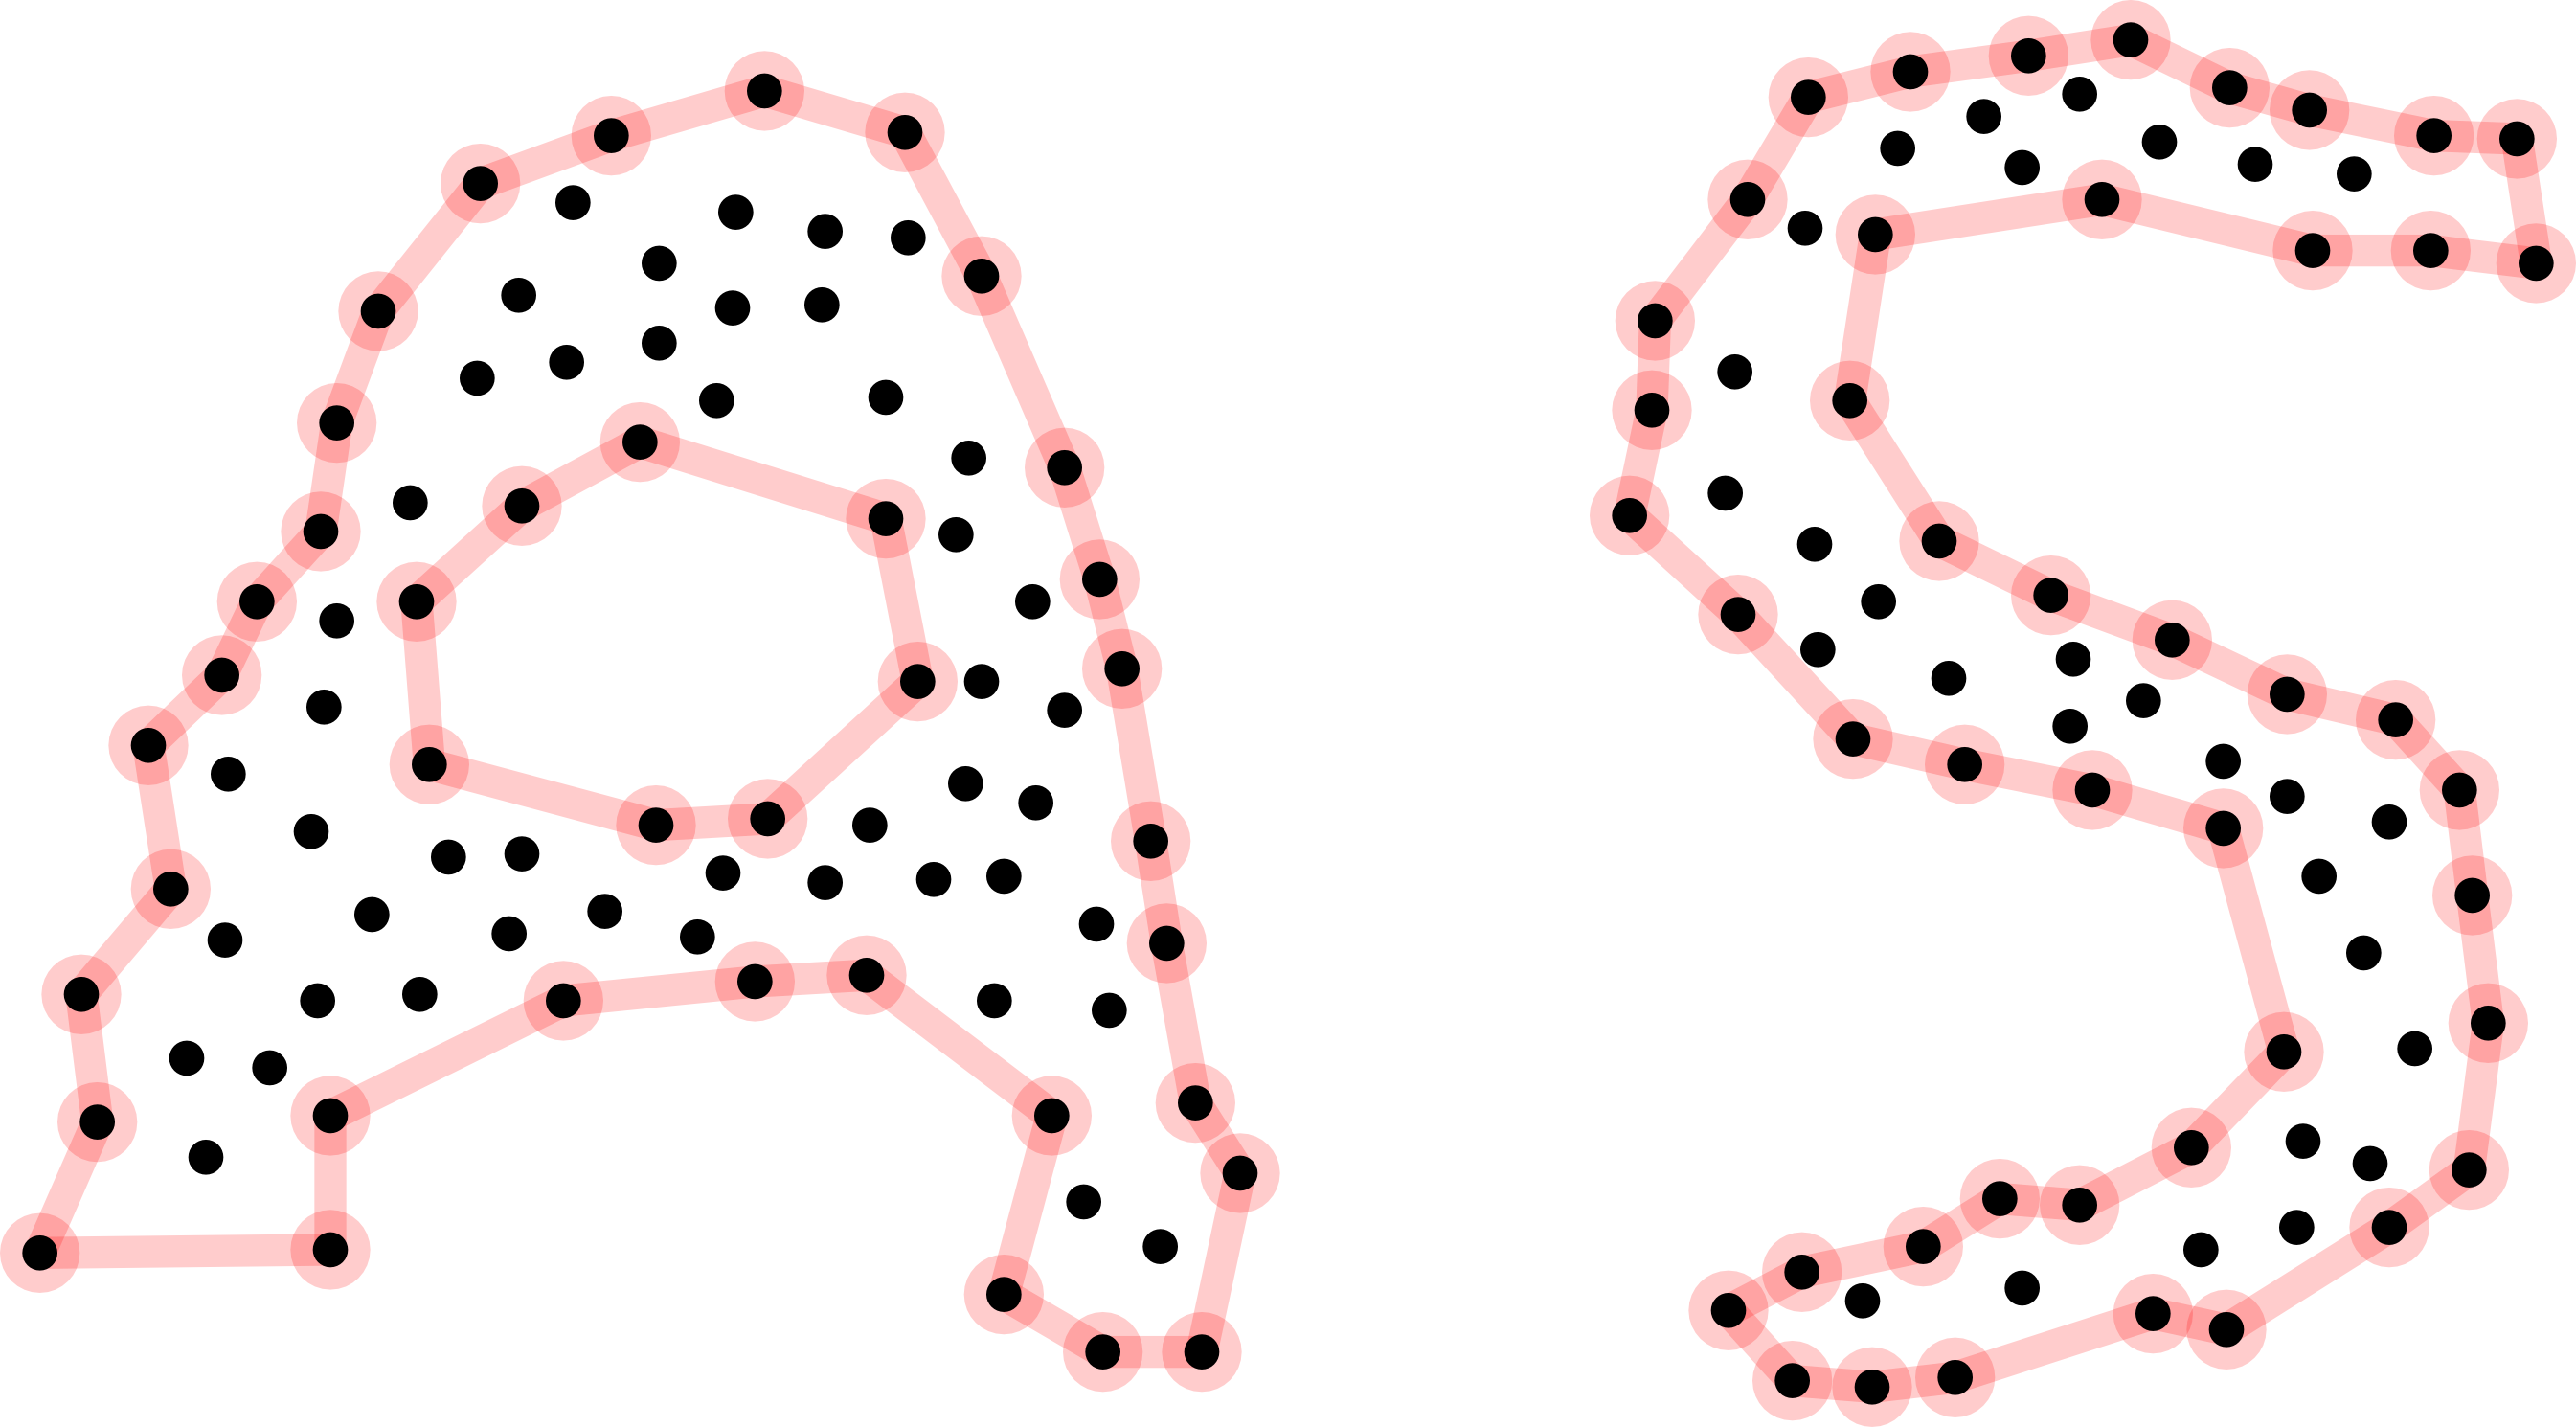
\includegraphics[scale=0.4]{../bilder/bigAS_shape.png}}
	\caption{$\alpha$-Shapes zweier Punktmengen}
	\label{fig:shapes}	
\end{figure}

In Abbildung~\ref{fig:alpha_shape} ist die $\alpha$-Shape einer einfachen Punktmenge dargestellt. Der zusammenhängende Graph verdeutlicht den Zusammenhang der einzelnen Punkte, so dass sich die Gestalt des Buchstabens $\alpha$ ergibt. In Abbildung~\ref{fig:bigAS_shape} ist die $\alpha$-Shape einer komplexen Punktmenge dargestellt. Der Graph ist nicht zusammenhängend. Die zusammenhängenden Teilgraphen begrenzen die Gestalt der Buchstaben A und S.

Die $\alpha$-Shape ist eng mit einer flächenmäßigen Darstellung der Gestalt einer Punktmenge verwandt, der $\alpha$-Hülle. Auch die $\alpha$-Hülle gruppiert Punkte nach dem Prinzip der Nähe und ist von demselben Parameter $\alpha$ abhängig.

\begin{figure}[htbp]
	\centering
	\subfloat[$\alpha$-Hülle einer einfachen Punktmenge\label{fig:alpha_hull}]
		{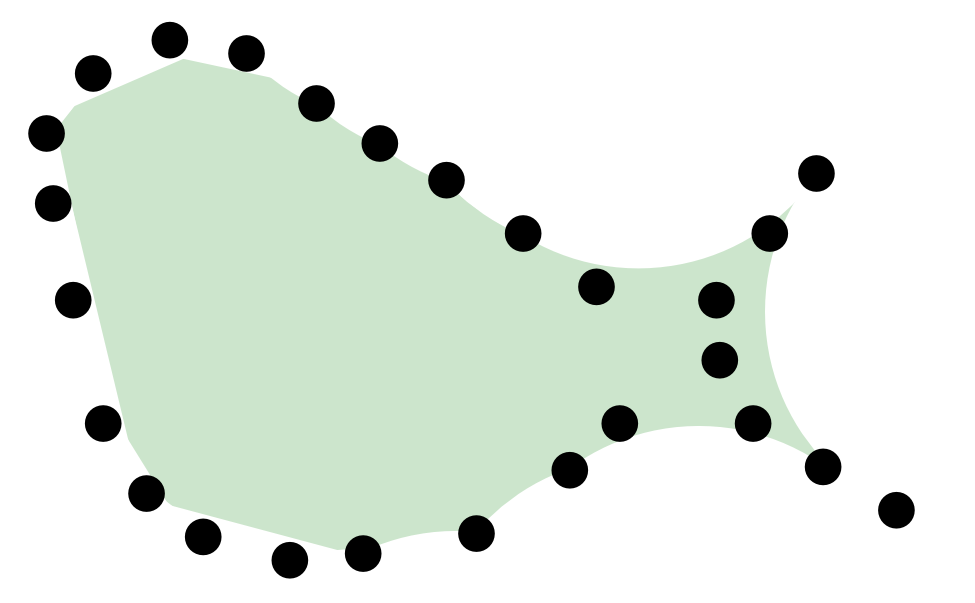
\includegraphics[scale=0.5]{../bilder/alpha_hull.png}}
	\qquad
	\subfloat[$\alpha$-Hülle einer komplexen Punktmenge\label{fig:bigAS_hull}]
		{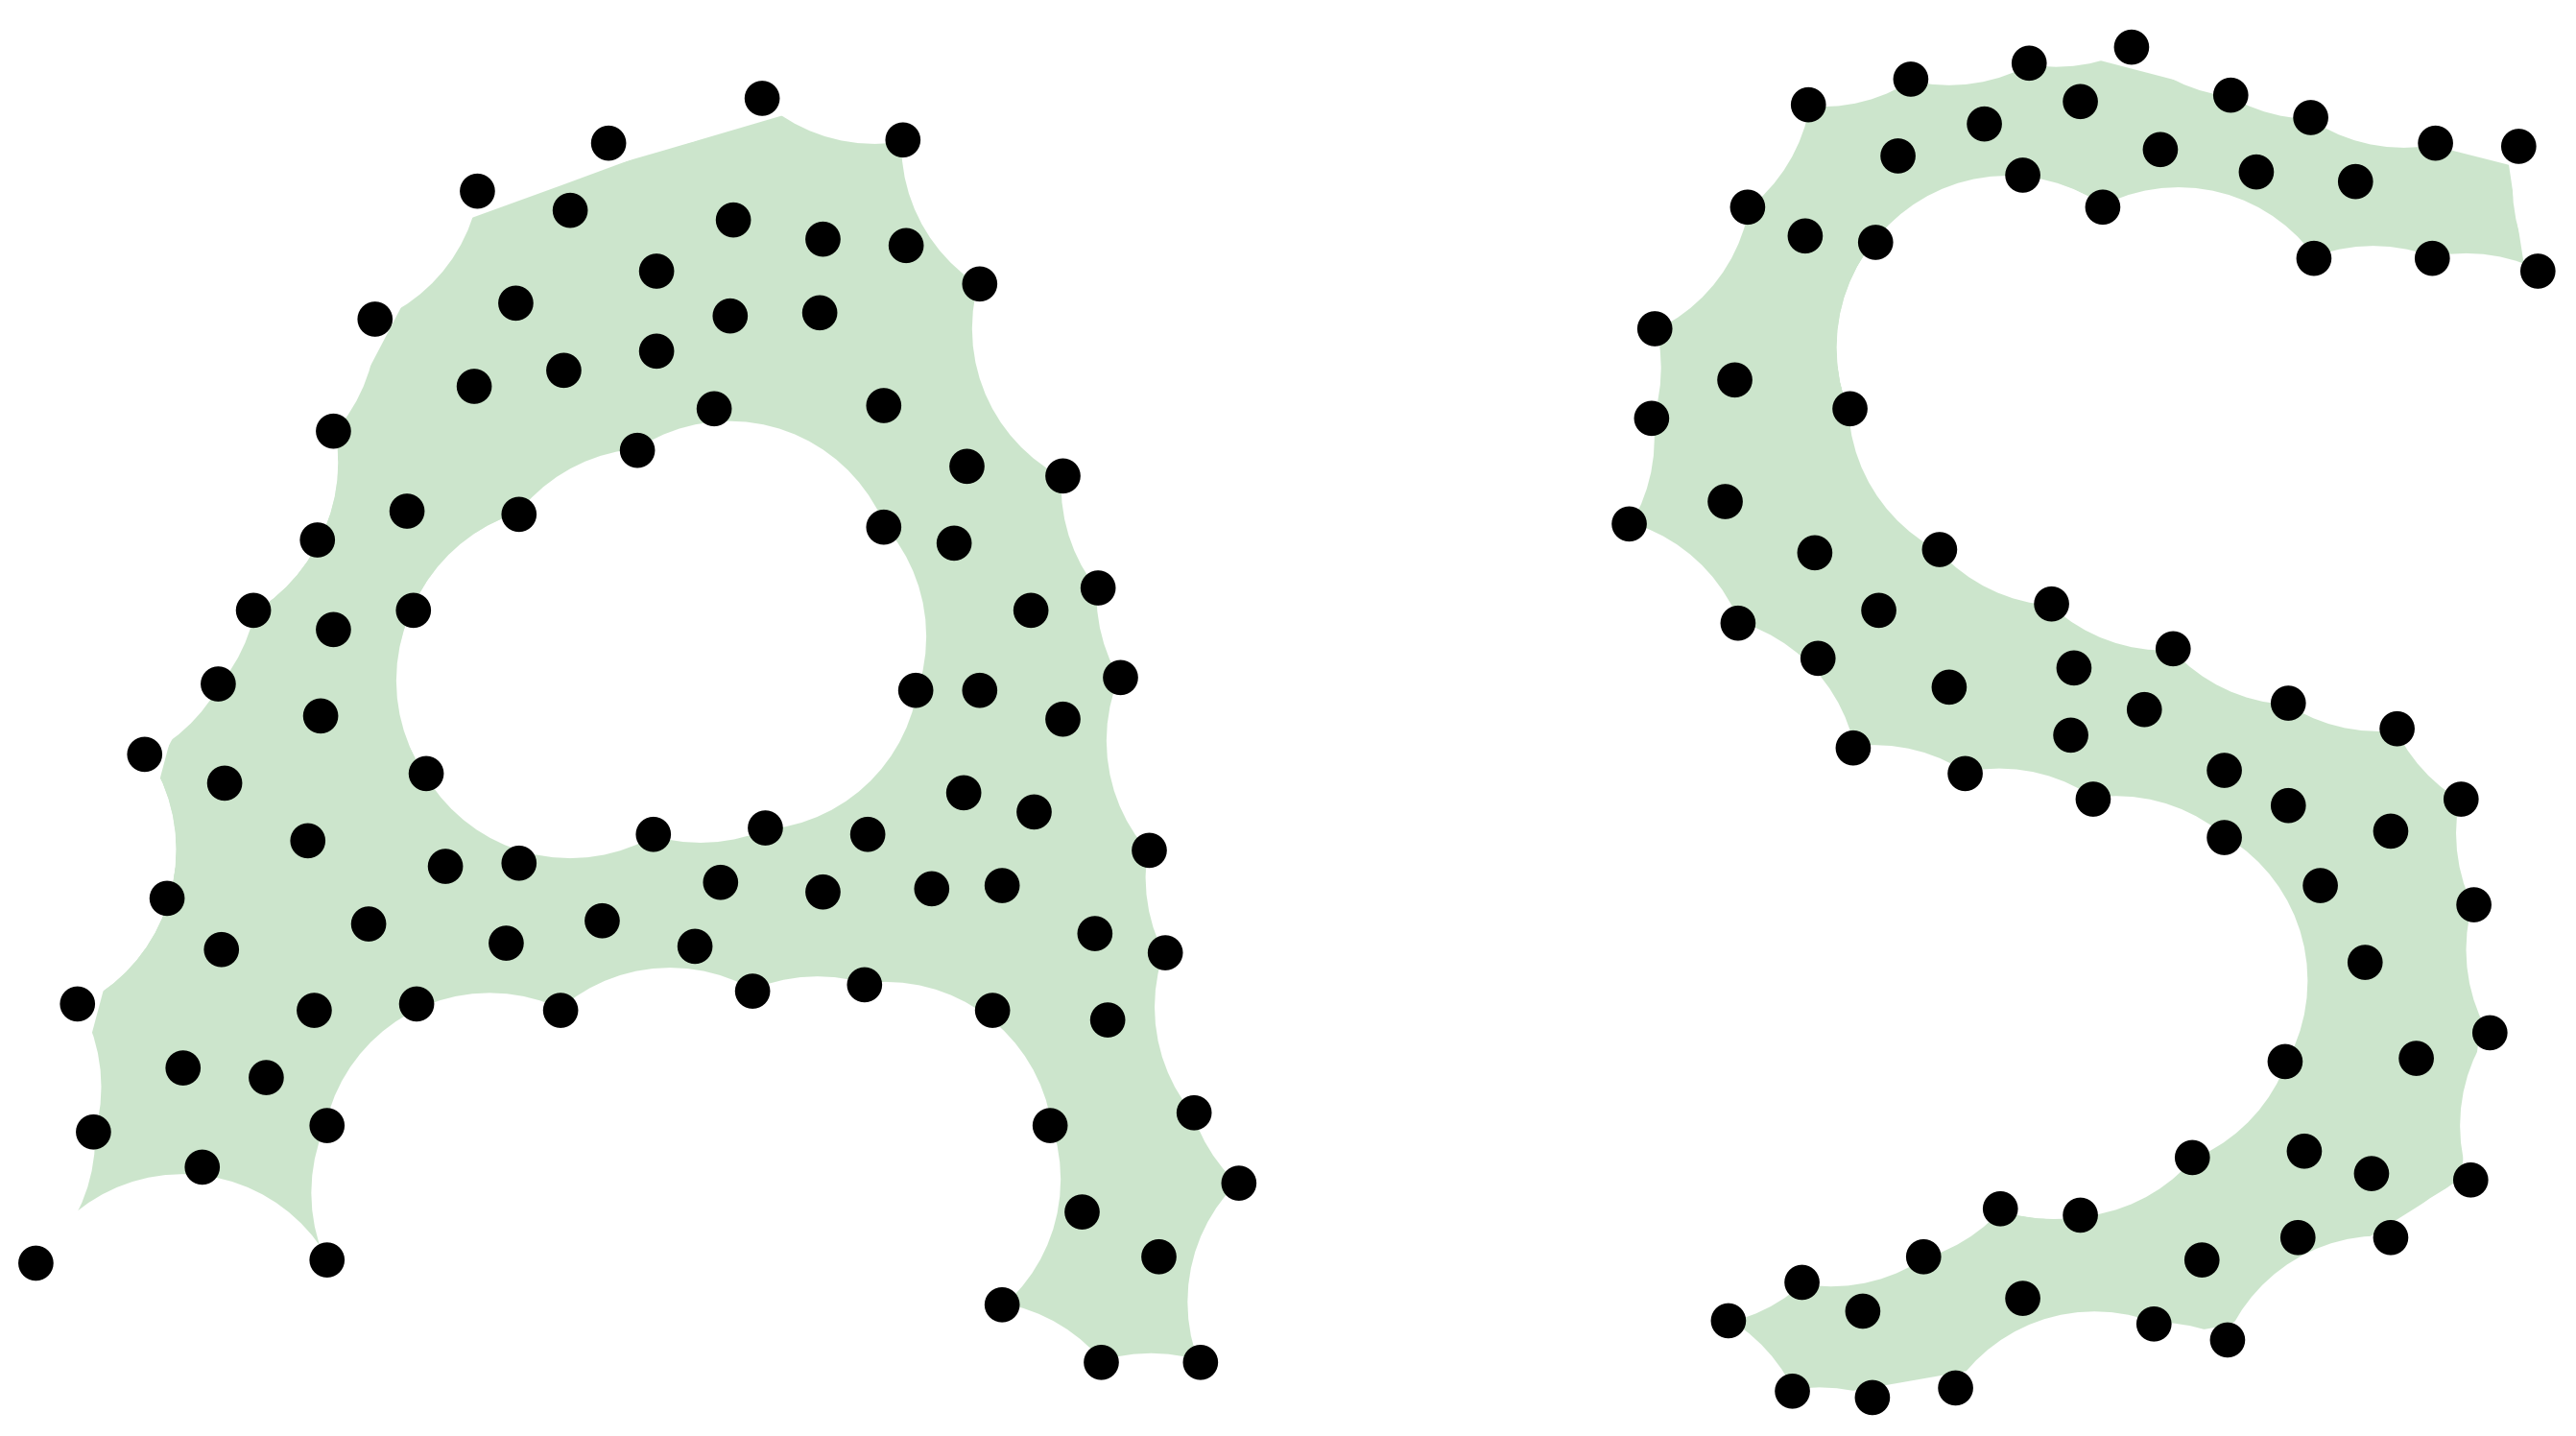
\includegraphics[scale=0.4]{../bilder/bigAS_hull.png}}
	\caption{$\alpha$-Hüllen zweier Punktmengen}
	\label{fig:hulls}	
\end{figure}

Abbildung~\ref{fig:hulls} zeigt $\alpha$-Hüllen für die Punktmengen aus Abbildung~\ref{fig:shapes}. Auch hier ist $\alpha$ wieder so gewählt worden, um eine möglichst gute Darstellung der durch die Punktmenge angenäherten Figuren zu erhalten.

% !TEX encoding = UTF-8 Unicode

\chapter{Die \boldmath{$\alpha$}-Shape}

Die $\alpha$-Shape wird mit Kreisscheiben mit einem Radius vom Betrag $\alpha$ bestimmt. Diese Kreisscheiben werden auch zur Konstruktion der $\alpha$-Hülle verwendet werden. Hier wird nun zuerst auf die $\alpha$-Hülle eingegangen und im Folgenden die $\alpha$-Shape definiert.

In \autocite{alpha1983} ist $\alpha$ der Kehrwert des Radius einer Kreisscheibe und es werden auch Komplemente dieser Kreisscheiben verwendet. In dieser Darstellung wurde auf die Verwendung der Komplemente von Kreisscheiben verzichtet.

Für die folgenden Definitionen sei eine Punktmenge $S$ gegeben. Die definierten Begriffe beziehen sich immer auf diese Punktmenge.

\section[Die $\alpha$-Hülle]{Die \boldmath{$\alpha$}-Hülle}

Die $\alpha$-Hülle ist abhängig von einem Parameter $\alpha$. Der Parameter $\alpha$ bestimmt dabei den Radius derjenigen Kreisscheiben, welche zu ihrer Konstruktion verwendet werden. Je nachdem ob $\alpha$ positiv oder negativ ist, wird die $\alpha$-Hülle unterschiedlich definiert. Für die verwendeten Kreisscheiben wird hier der Begriff der $\alpha$-Kreisscheibe eingeführt.

\begin{defin}
Für $\alpha > 0$ ist eine offene Kreisscheibe mit Radius $\alpha$ eine \emph{$\alpha$-Kreisscheibe}, genau dann wenn diese keinen Punkt aus $S$ enthält. Eine solche Kreisscheibe wird auch \emph{positive $\alpha$-Kreisscheibe} genannt.\\
Für $\alpha < 0$ ist eine abgeschlossene Kreisscheibe mit einem Radius vom Betrag $\alpha$ eine \emph{$\alpha$-Kreisscheibe}, genau dann wenn diese alle Punkte aus $S$ enthält. Eine solche Kreisscheibe wird auch \emph{negative $\alpha$-Kreisscheibe} genannt.
\end{defin}

\begin{figure}[htbp]
	\centering
	\subfloat[Positive $\alpha$-Kreisscheibe\label{fig:alphaDisc_positive}]
		{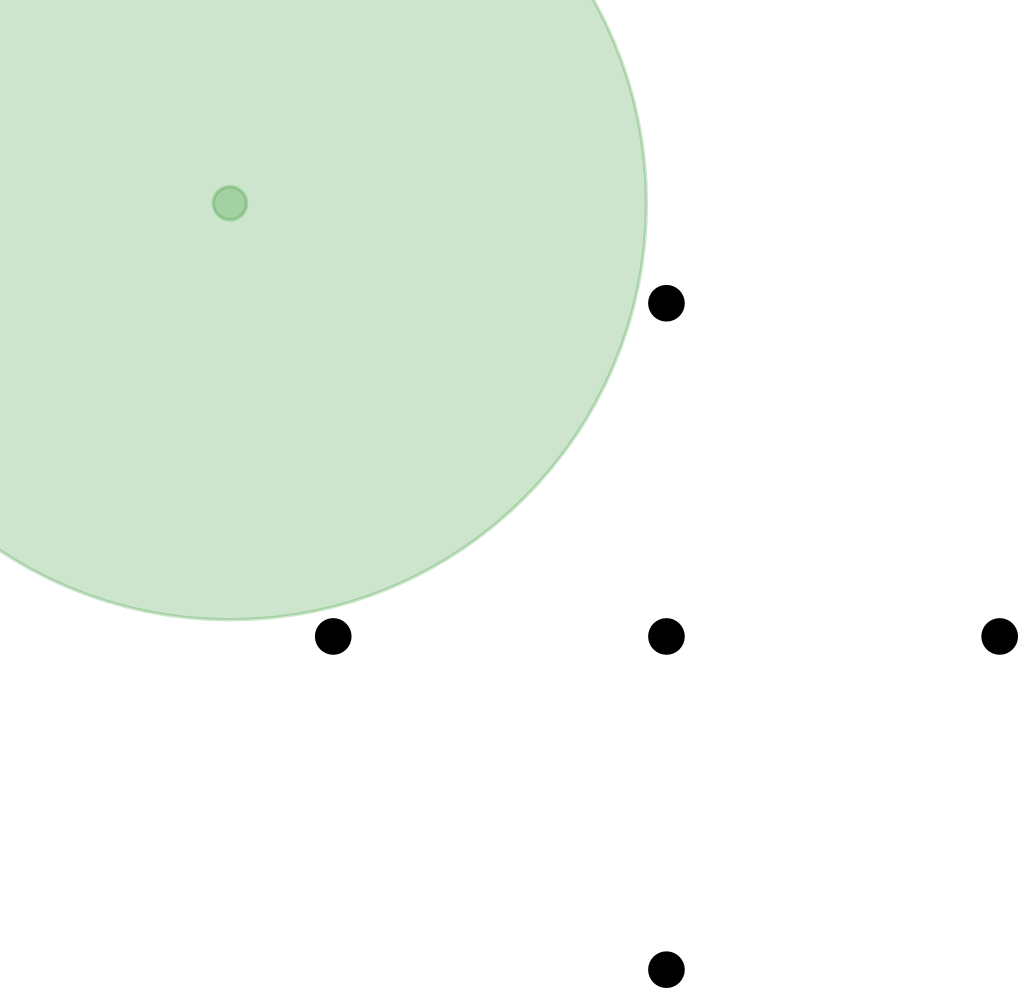
\includegraphics[scale=0.7]{../bilder/alphaDisc_positive.png}}
	\hspace{2cm}
	\subfloat[Negative $\alpha$-Kreisscheibe\label{fig:alphaDisc_negative}]
		{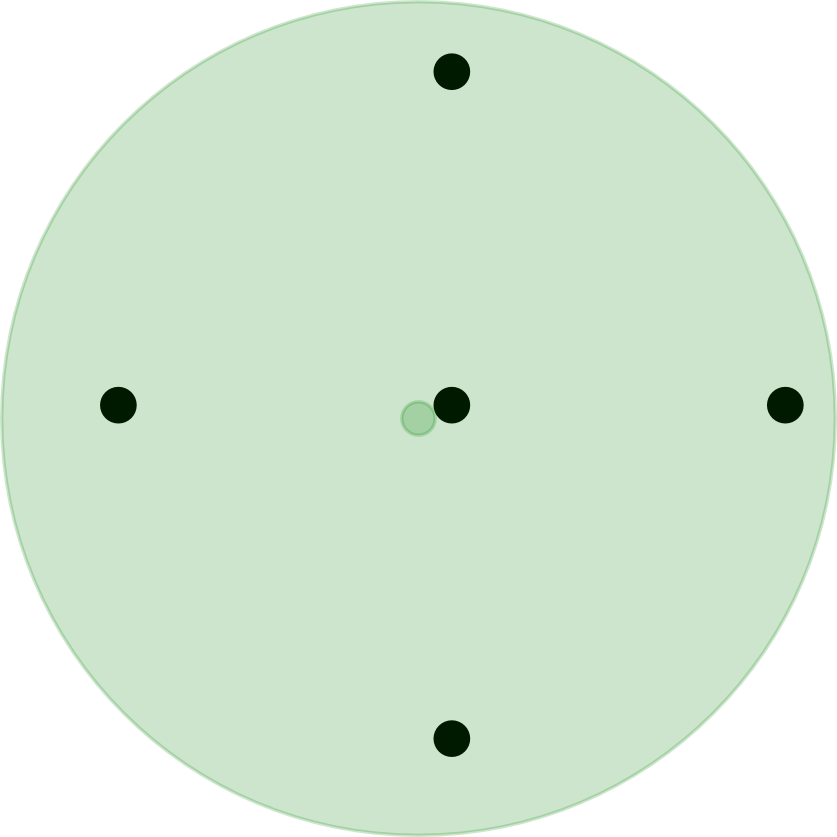
\includegraphics[scale=0.7]{../bilder/alphaDisc_negative.png}}
	\caption{$\alpha$-Kreisscheiben}
	\label{fig:alphaDiscs}	
\end{figure}

In Abbildung~\ref{fig:alphaDiscs} sind $\alpha$-Kreisscheiben mit betragsmäßig gleichem Radius dargestellt. Abbildung~\ref{fig:alphaDisc_positive} stellt eine positive $\alpha$-Kreisscheibe dar und Abbildung~\ref{fig:alphaDisc_negative} eine negative.

Mit Hilfe der $\alpha$-Kreisscheiben wird nun die $\alpha$-Hülle definiert.

\begin{defin}
Für $\alpha > 0$ ist die \emph{$\alpha$-Hülle} gleich dem Komplement der Vereinigung aller $\alpha$-Kreisscheiben. Diese $\alpha$-Hülle wird auch \emph{positive $\alpha$-Hülle} genannt.\\
Für $\alpha < 0$ ist die $\alpha$-Hülle gleich der Schnittfläche aller $\alpha$-Kreisscheiben. Diese $\alpha$-Hülle wird auch \emph{negative $\alpha$-Hülle} genannt.
\end{defin}

Existieren für ein $\alpha < 0$ keine $\alpha$-Kreisscheiben, so ist die $\alpha$-Hülle gleich der Ebene.

\begin{figure}[htbp]
	\centering
	\subfloat[Positive $\alpha$-Hülle\label{fig:alphaHull_positive}]
		{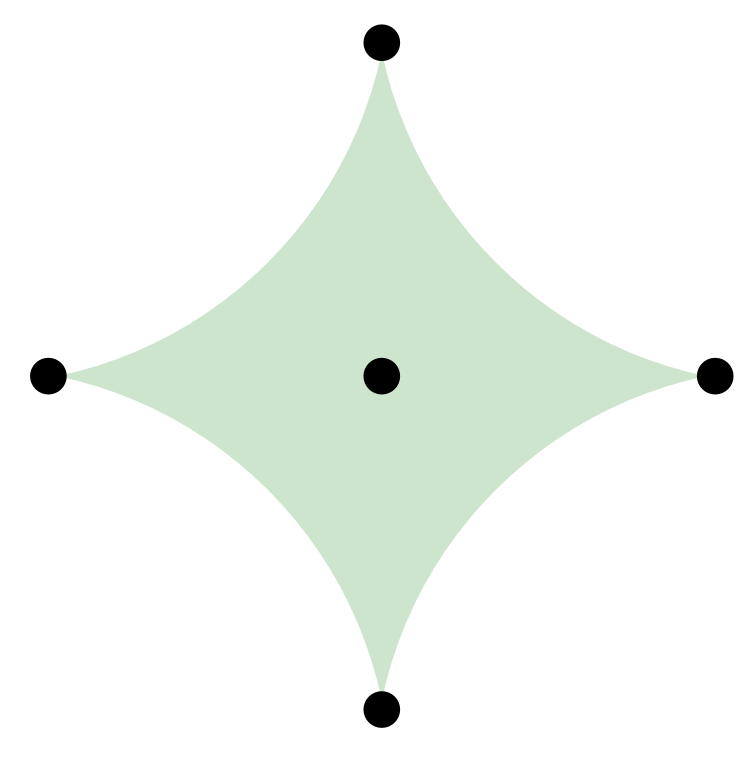
\includegraphics[scale=0.7]{../bilder/alphaHull_positive.png}}
	\hspace{2cm}
	\subfloat[Negative $\alpha$-Hülle\label{fig:alphaHull_negative}]
		{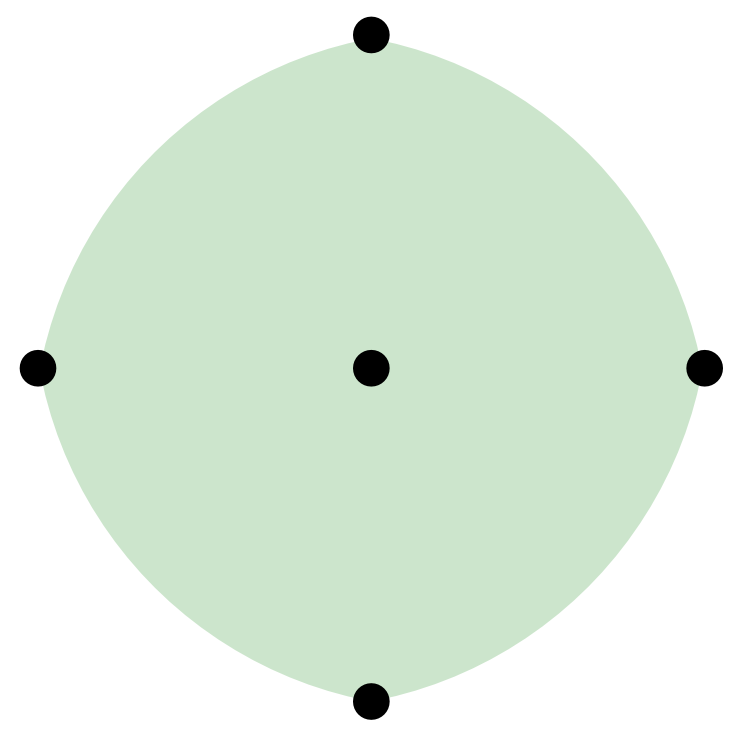
\includegraphics[scale=0.7]{../bilder/alphaHull_negative.png}}
	\caption{$\alpha$-Hüllen}
	\label{fig:alphaHulls}	
\end{figure}

In Abbildung~\ref{fig:alphaHulls} sind positive und negative $\alpha$-Hüllen dargestellt. Der Radius der $\alpha$-Kreisscheiben ist gleich derer in Abbildung~\ref{fig:alphaDiscs}.

Die $\alpha$-Hülle kann auch als Verallgemeinerung der konvexen Hülle betrachtet werden. Für betragsmäßig unendlich große $\alpha$ werden die $\alpha$-Kreisscheiben zu Halbebenen. Dann ist die $\alpha$-Hülle gleich der konvexen Hülle.

\begin{defin}
Die \emph{konvexe Hülle} ist die Schnittfläche aller abgeschlossenen Halbebenen, welche alle Punkte aus $S$ beinhalten.\\
Alternativ kann die konvexe Hülle auch als Komplement zur Vereinigung aller offenen Halbebenen, welche keinen Punkt aus $S$ beinhalten, betrachtet werden.
\end{defin}

\begin{figure}[htbp]
	\centering
	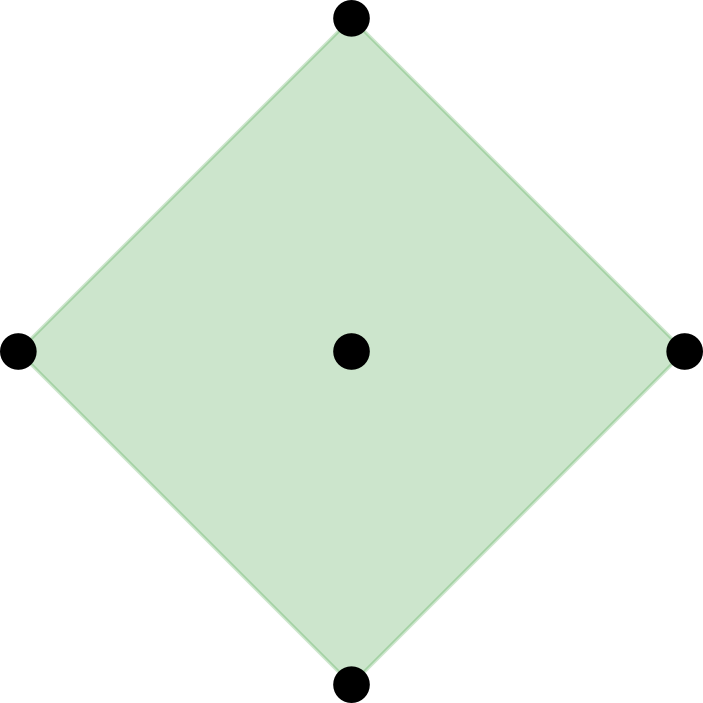
\includegraphics[scale=0.7]{../bilder/convexHull.png}
	\caption{Konvexe Hülle}
	\label{fig:convexHull}	
\end{figure}

In Abbildung~\ref{fig:convexHull} ist die konvexe Hülle der in Abbildung~\ref{fig:alphaDiscs} und \ref{fig:alphaHulls} verwendeten Punktmenge dargestellt.

\section[Die $\alpha$-Shape]{Die \boldmath{$\alpha$}-Shape}

Die $\alpha$-Shape ist ein Graph, dessen Knotenmenge eine Teilmenge von $S$ ist. Knoten der $\alpha$-Shape werden $\alpha$-extreme Punkte genannt.

\begin{defin}
Ein Punkt aus $S$ ist \emph{$\alpha$-extrem}, genau dann wenn er auf dem Rand einer $\alpha$-Kreisscheibe liegt.
\end{defin}

\begin{figure}[htbp]
	\centering
	\subfloat[$\alpha$-extremer Punkt auf positiver $\alpha$-Kreisscheibe\label{fig:alphaExtreme_positive}]
		{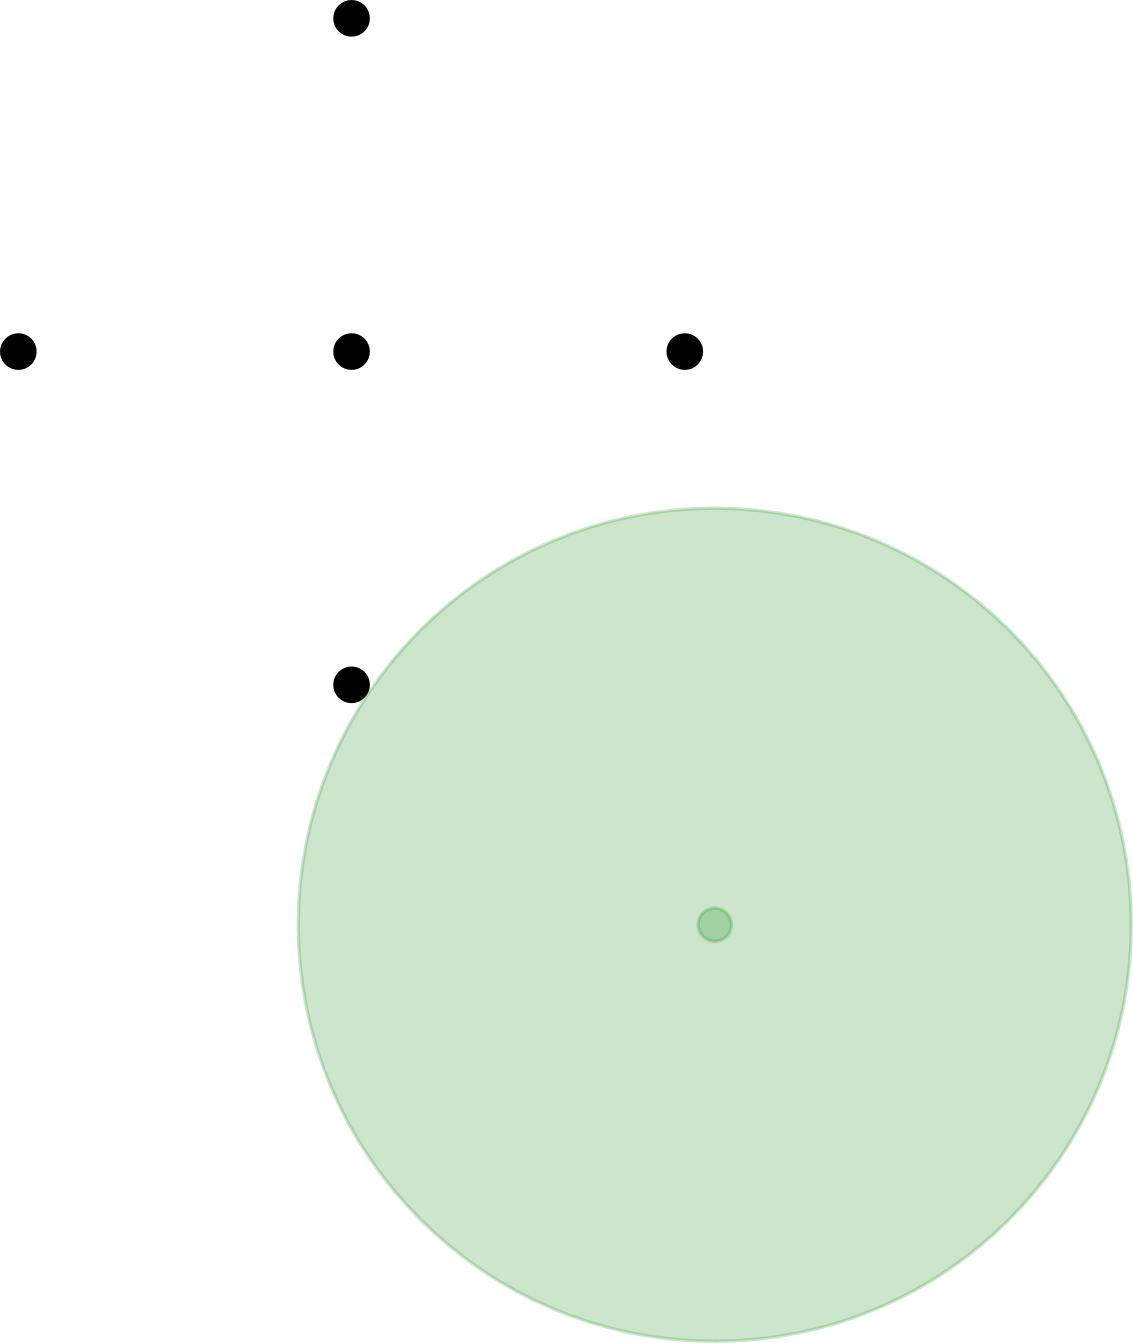
\includegraphics[scale=0.7]{../bilder/alphaExtreme_positive.png}}
	\hspace{2cm}
	\subfloat[$\alpha$-extremer Punkt auf negativer $\alpha$-Kreisscheibe\label{fig:alphaExtreme_negative}]
		{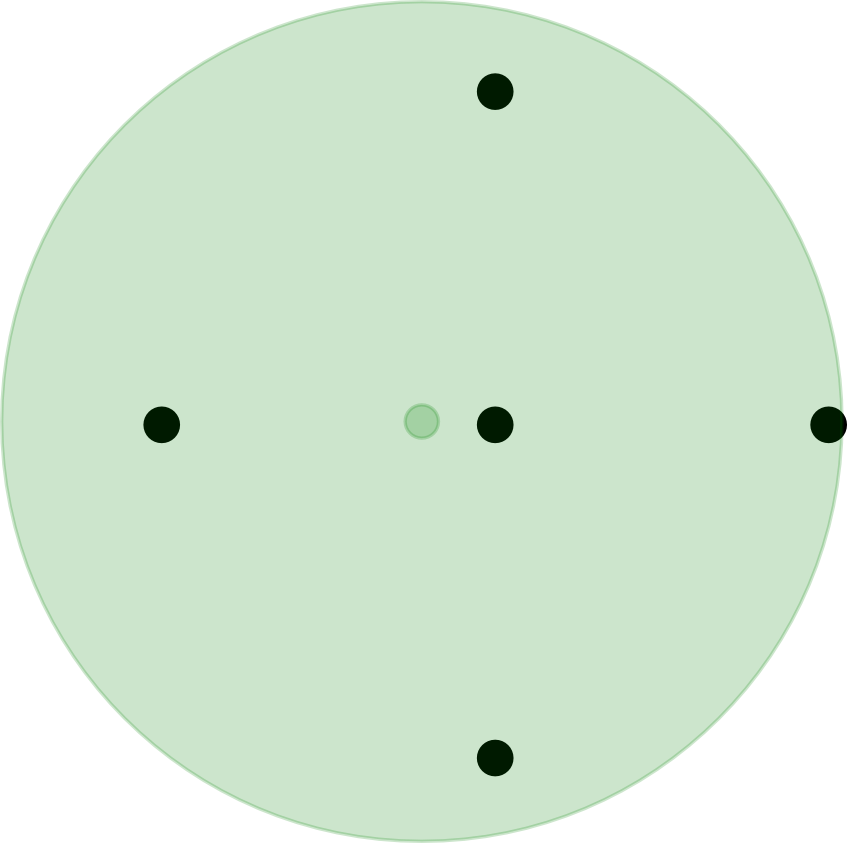
\includegraphics[scale=0.7]{../bilder/alphaExtreme_negative.png}}
	\caption{$\alpha$-extreme Punkte}
	\label{fig:alphaExtremes}	
\end{figure}

Abbildung~\ref{fig:alphaExtremes} zeigt $\alpha$-extreme Punkte auf dem Rand von positiven und negativen $\alpha$-Kreisscheiben.

\begin{defin}
Zwei Punkte aus $S$ sind \emph{$\alpha$-Nachbarn}, genau dann wenn sie auf dem Rand derselben $\alpha$-Kreisscheibe liegen und auf dieser direkt benachbart sind.
\end{defin}

\begin{figure}[htbp]
	\centering
	\subfloat[$\alpha$-Nachbarn auf positiver $\alpha$-Kreisscheibe\label{fig:alphaNeighbours_positive}]
		{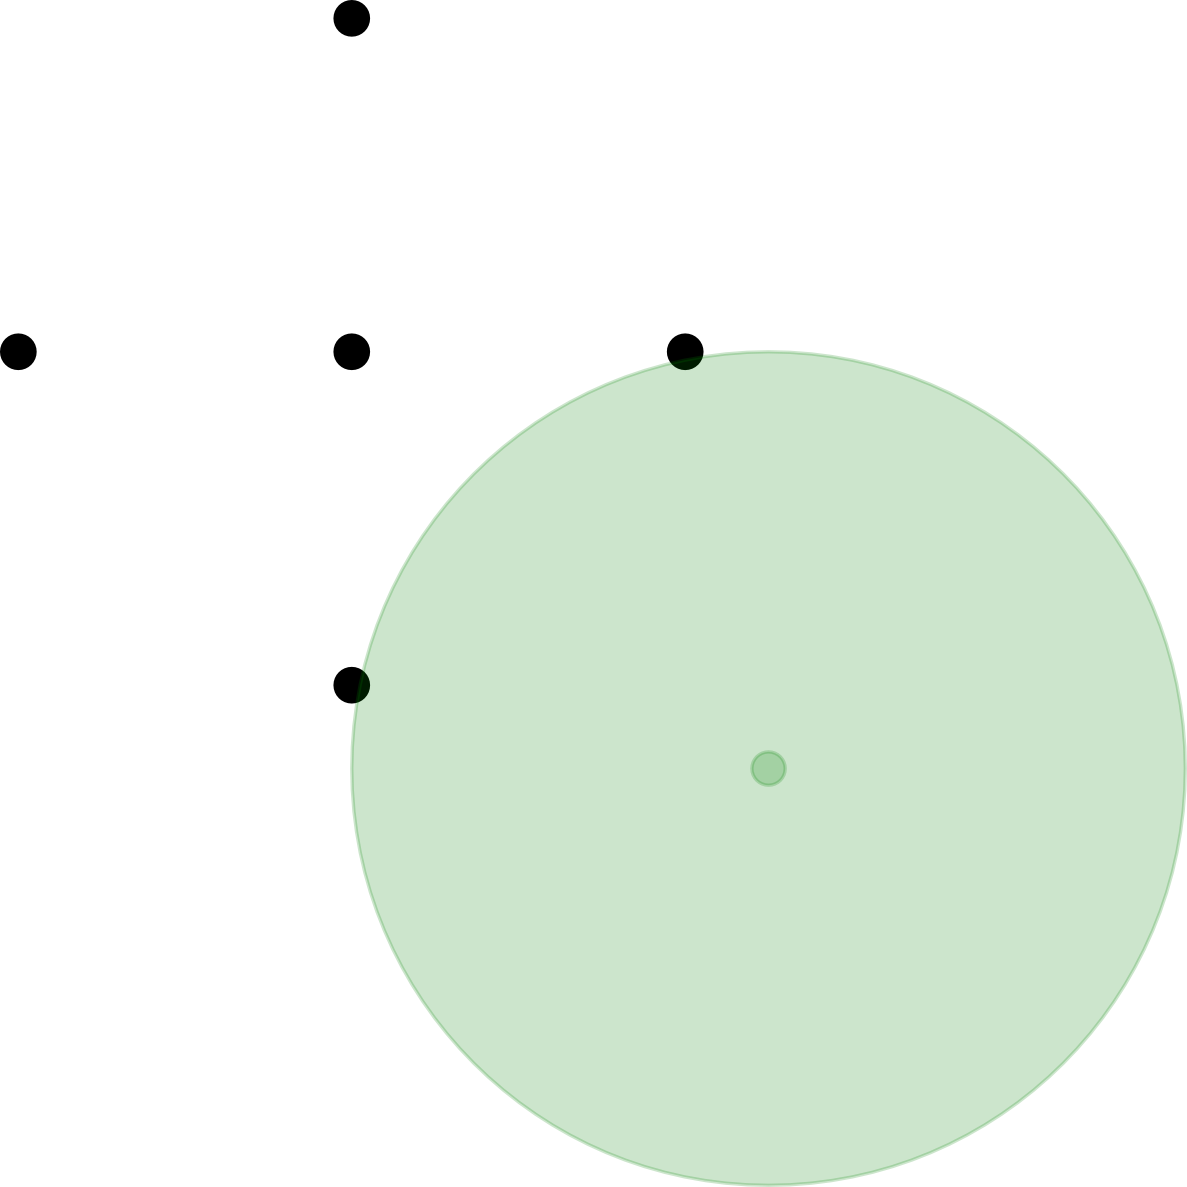
\includegraphics[scale=0.7]{../bilder/alphaNeighbours_positive.png}}
	\hspace{2cm}
	\subfloat[$\alpha$-Nachbarn auf negativer $\alpha$-Kreisscheibe\label{fig:alphaNeighbours_negative}]
		{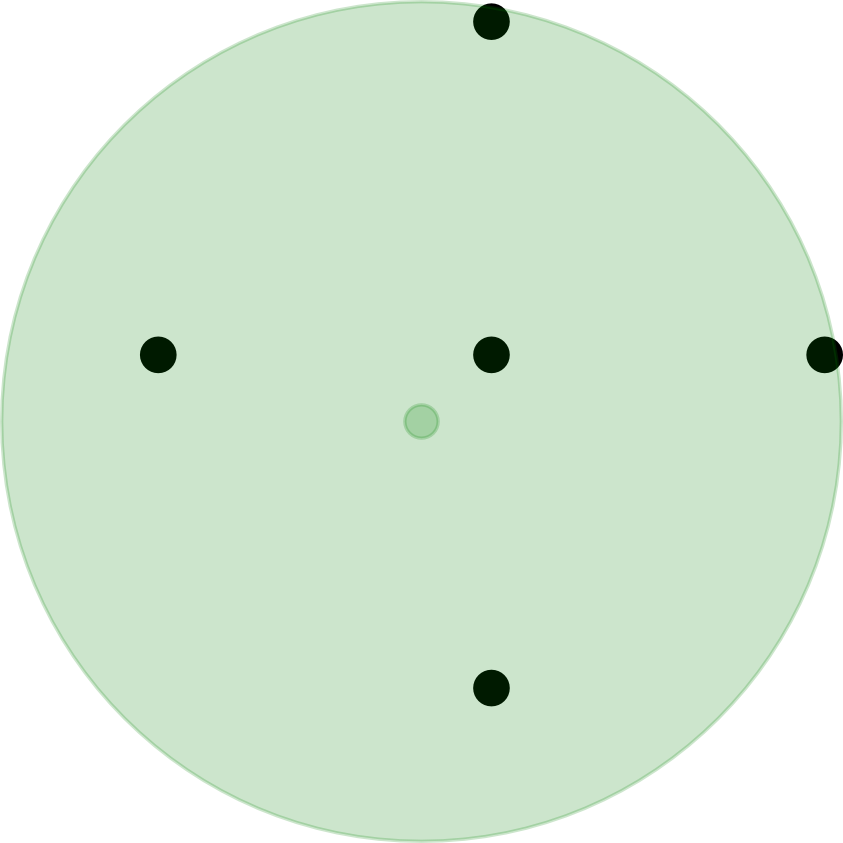
\includegraphics[scale=0.7]{../bilder/alphaNeighbours_negative.png}}
	\caption{$\alpha$-Nachbarn}
	\label{fig:alphaNeighbours}	
\end{figure}

Abbildung~\ref{fig:alphaNeighbours} zeigt $\alpha$-Nachbarn, welche jeweils auf einer positiven und einer negativen $\alpha$-Kreisscheibe liegen.

Mit Hilfe $\alpha$-extremer Punkte und $\alpha$-Nachbarn wird die $\alpha$-Shape folgendermaßen definiert.

\begin{defin}
Die \emph{$\alpha$-Shape} ist der Graph mit $\alpha$-extremen Punkten als Knoten und Kanten zwischen den $\alpha$-Nachbarn. Für ein $\alpha > 0$ wird die $\alpha$-Shape auch \emph{positive $\alpha$-Shape} genannt. Für ein $\alpha < 0$ wird die $\alpha$-Shape auch \emph{negative $\alpha$-Shape} genannt.
\end{defin}

\begin{figure}[htbp]
	\centering
	\subfloat[Positive $\alpha$-Shape\label{fig:alphaShape_positive}]
		{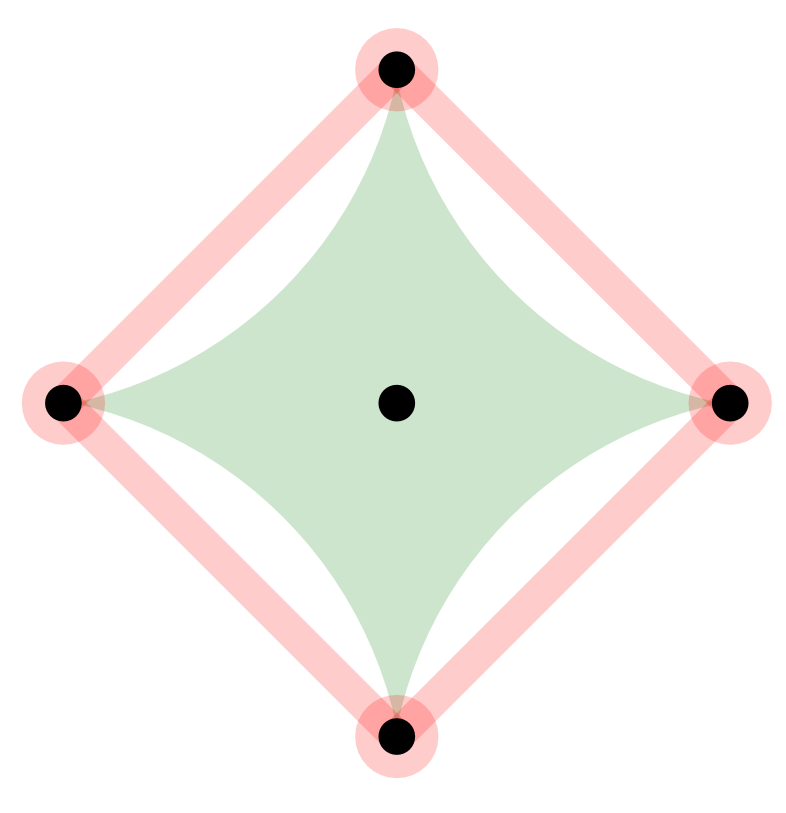
\includegraphics[scale=0.7]{../bilder/alphaShape_positive.png}}
	\hspace{2cm}
	\subfloat[Negative $\alpha$-Shape\label{fig:alphaShape_negative}]
		{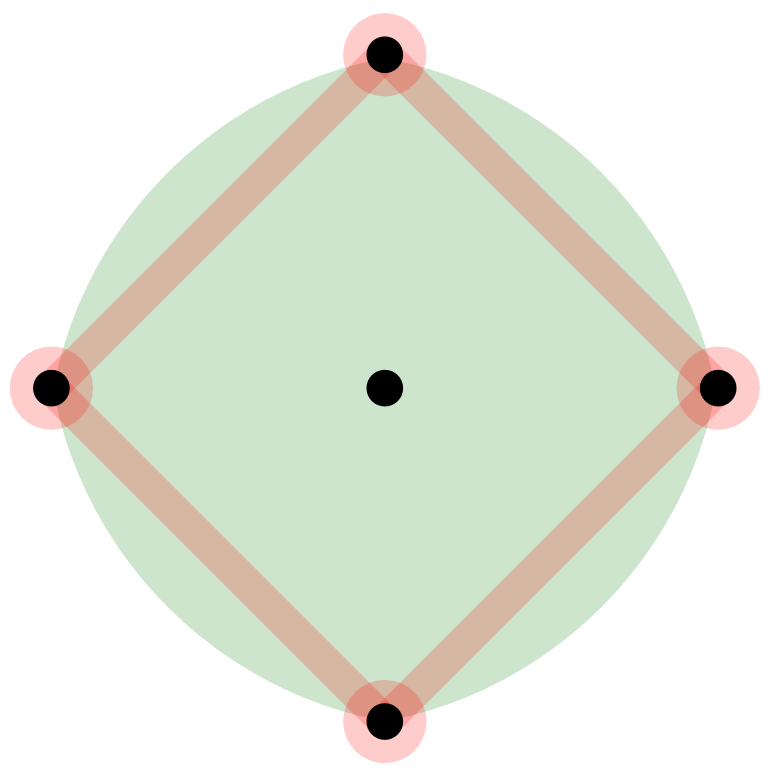
\includegraphics[scale=0.7]{../bilder/alphaShape_negative.png}}
	\caption{$\alpha$-Shapes}
	\label{fig:alphaShapes}	
\end{figure}

In Abbildung~\ref{fig:alphaShapes} sind positive und negative $\alpha$-Shapes und -Hüllen abgebildet.

Dadurch, dass nur Punkte, welche direkt auf einer $\alpha$-Kreisscheibe benachbart sind auch $\alpha$-Nachbarn sind, kreuzen sich Kanten der $\alpha$-Shape nicht.

\section[$\alpha$-Hüllen und -Shapes für verschiedene $\alpha$]{\boldmath{$\alpha$}-Hüllen und -Shapes für verschiedene \boldmath{$\alpha$}}

Für die folgenden Beispiele wird der Parameter $\alpha$ von betragsmäßig unendlich großen, negativen hin zu unendlich großen, positiven Werten variiert.

Für betragsmäßig unendlich große, negative Werte von $\alpha$ ist die $\alpha$-Hülle gleich der konvexen Hülle. Die $\alpha$-Shape liegt in diesem Fall auf dem Rand der konvexen Hülle.

\begin{figure}[htbp]
	\centering
	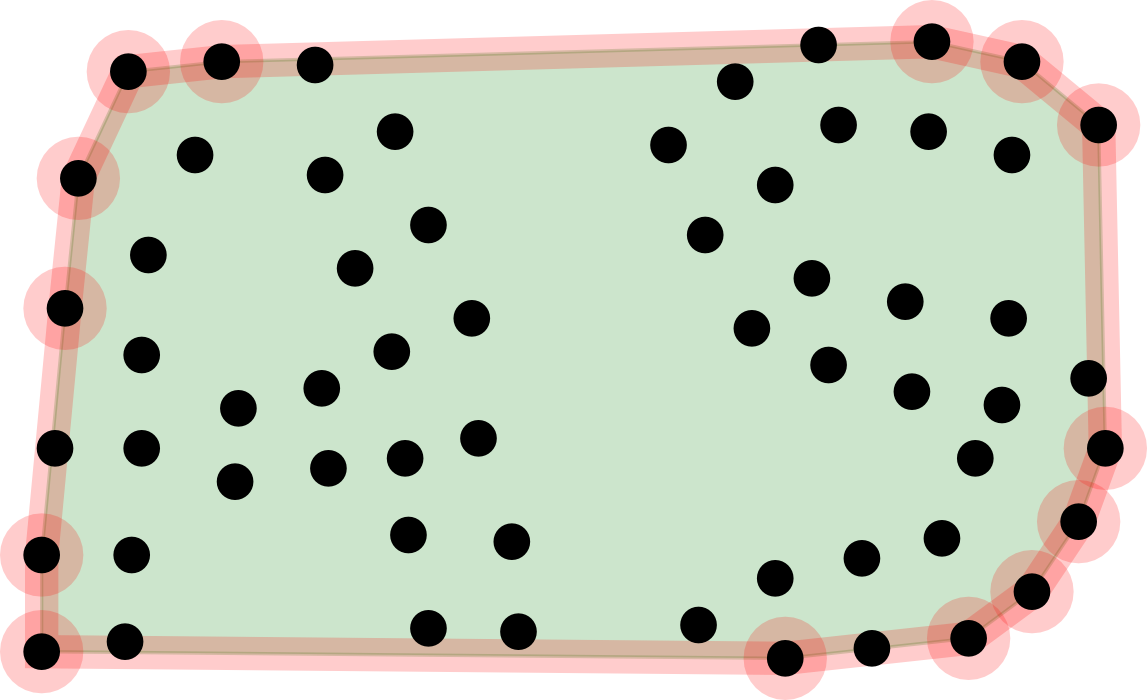
\includegraphics[scale=0.7]{../bilder/smallAS_shapeHull_convex.png}
	\caption{$\alpha$-Hülle gleich der konvexen Hülle}
	\label{fig:shapeHull_convex}
\end{figure}

Abbildung~\ref{fig:shapeHull_convex} stellt $\alpha$-Hülle und -Shape für den Fall dar, dass die $\alpha$-Hülle gleich der konvexen Hülle ist.

Bewegt sich $\alpha$ von betragsmäßig sehr großen, negativen Werten hin zu betragsmäßig kleineren, negativen Werten, so dehnt sich die $\alpha$-Hülle aus. Punkte aus $S$, welche für betragsmäßig größere $\alpha$ noch auf dem Rand der $\alpha$-Hülle gelegen sind, befinden sich nun im inneren der $\alpha$-Hülle. Diese Punkte sind somit nicht mehr $\alpha$-extrem und tragen nicht mehr zu $\alpha$-Shape bei.

\begin{figure}[htbp]
	\centering
	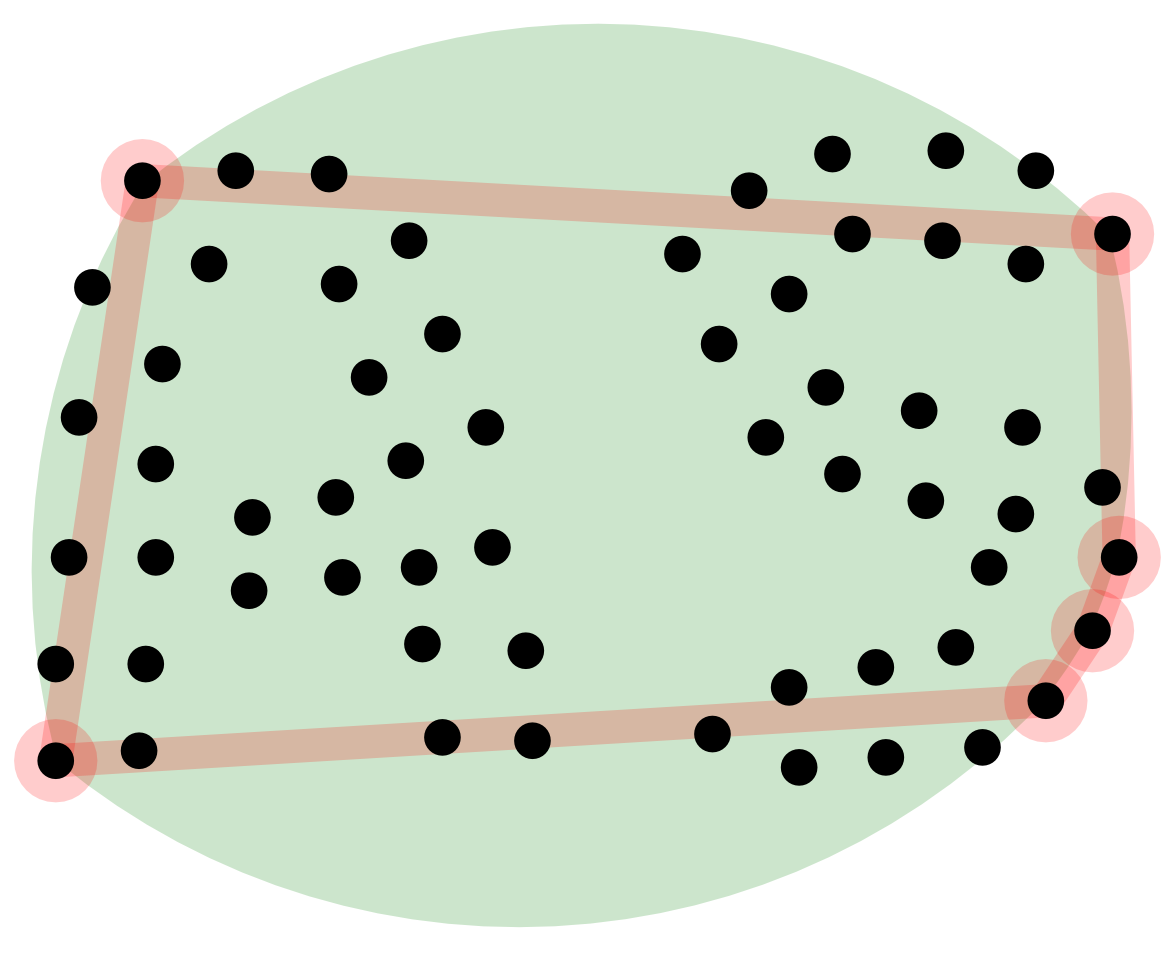
\includegraphics[scale=0.7]{../bilder/smallAS_shapeHull_negative.png}
	\caption{$\alpha$-Hülle und -Shape für negatives $\alpha$}
	\label{fig:shapeHull_negative}
\end{figure}

Abbildung~\ref{fig:shapeHull_negative} stellt den gerade geschilderten Fall einer $\alpha$-Shape und einer $\alpha$-Hülle dar.

Nun sei $\alpha$ gleich der Negation des Radius des kleinsten einschließenden Kreises der Punktmenge. In diesem Fall entspricht die $\alpha$-Hülle gleich der kleinsten negativen $\alpha$-Kreisscheibe. Diese Kreisscheibe wird von dem kleinsten einschließenden Kreis umrandet. Die Knotenmenge der $\alpha$-Shape ist die Menge derjenigen Punkte aus $S$, welche auf diesem Kreis liegen. Die Kanten der $\alpha$-Shape verbinden diejenigen Knoten, welche auf dem Kreis direkt benachbart sind.

\begin{figure}[htbp]
	\centering
	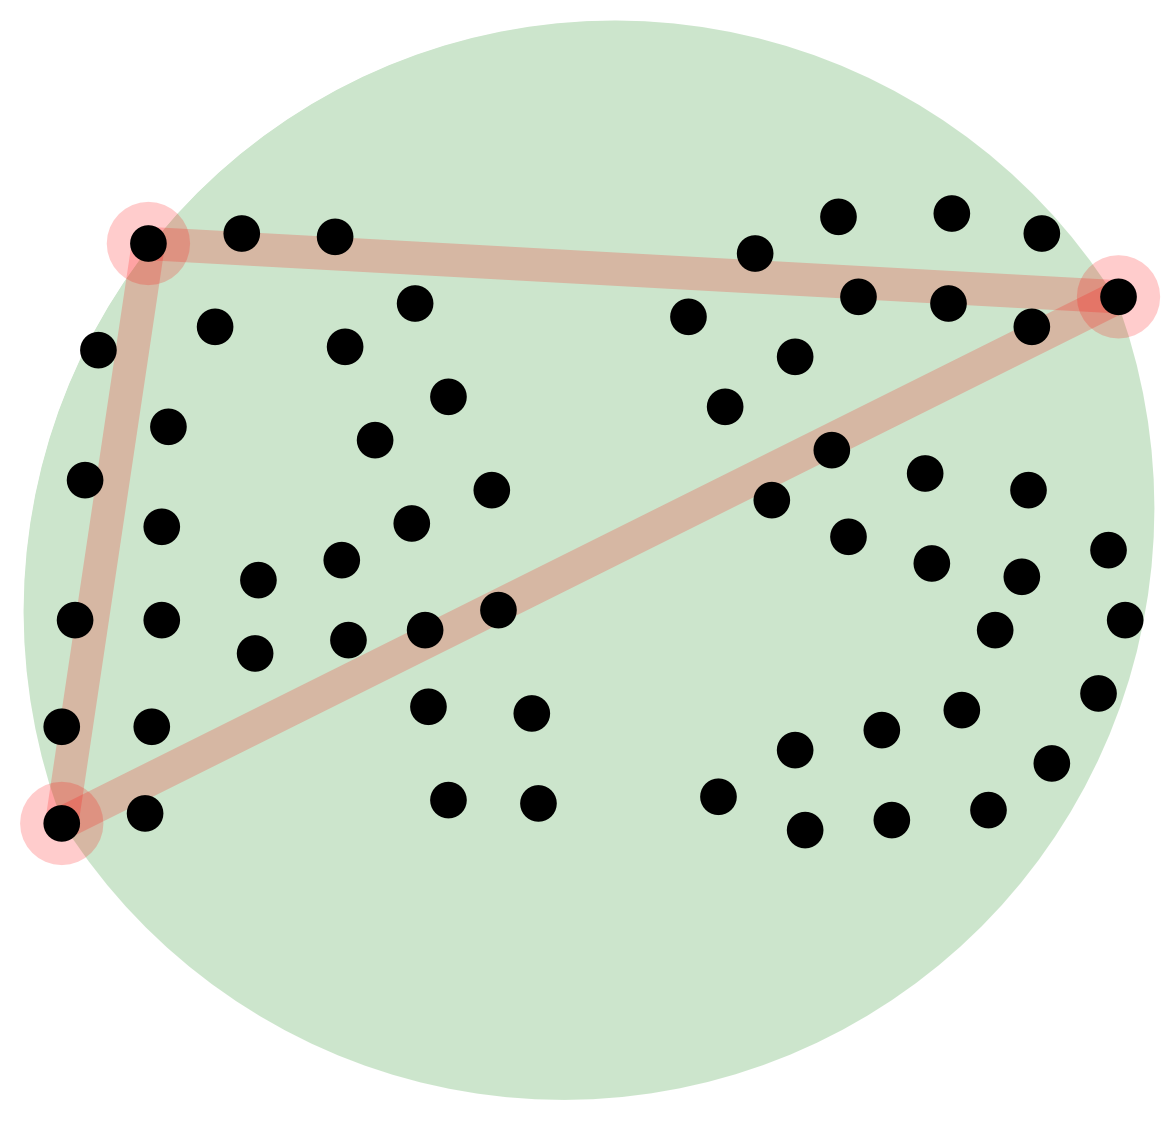
\includegraphics[scale=0.7]{../bilder/smallAS_shapeHull_smallestCircle.png}
	\caption{$\alpha$-Hülle gleich kleinster negativer $\alpha$-Kreisscheibe}
	\label{fig:shapeHull_smallestCircle}
\end{figure}

Abbildung~\ref{fig:shapeHull_smallestCircle} stellt einen Fall dar, indem drei Punkte auf der kleinsten möglichen negativen $\alpha$-Kreisscheibe liegen. Dies sind die $\alpha$-extremen Punkte, von denen jedes Paar auch $\alpha$-Nachbarn sind.

Für negative $\alpha$, welche vom Betrag her kleiner sind als der Radius des kleinsten einschließenden Kreises, existiert keine $\alpha$-Kreisscheibe mehr. Die $\alpha$-Hülle besteht nunmehr aus der gesamten Ebene. Die $\alpha$-Shape enthält keine Knoten und keine Kanten, da keine $\alpha$-extremen Punkte und somit auch keine $\alpha$-Nachbarn existieren.

Für ein $\alpha = 0$ sind $\alpha$-Hülle und -Shape nicht definiert.

Ist ein positives $\alpha$ kleiner als die Hälfte des Abstands des dichtesten Paares, so ist die $\alpha$-Hülle leer. Die Vereinigung der $\alpha$-Kreisscheiben füllt die gesamte Ebene aus. Die $\alpha$-Hülle ist das Komplement dieser Vereinigung, also leer. Die Knotenmenge der $\alpha$-Shape ist die gesamte Punktmenge $S$, da jeder Punkt aus $S$ auf dem Rand einer $\alpha$-Kreisscheibe liegt. Die Kantenmenge ist leer, da es keine zwei Punkte gibt, welche auf dem Rand derselben $\alpha$-Kreisscheibe liegen.

Für ein sehr kleines positives $\alpha$, welches gleich der Hälfte des Abstands des dichtesten Paares ist, ist die Kantenmenge der $\alpha$-Shape nicht mehr leer. Es gibt mindestens ein dichtestes Paar, welches auf dem Rand derselben $\alpha$-Kreisscheibe liegt.

\begin{figure}[htbp]
	\centering
	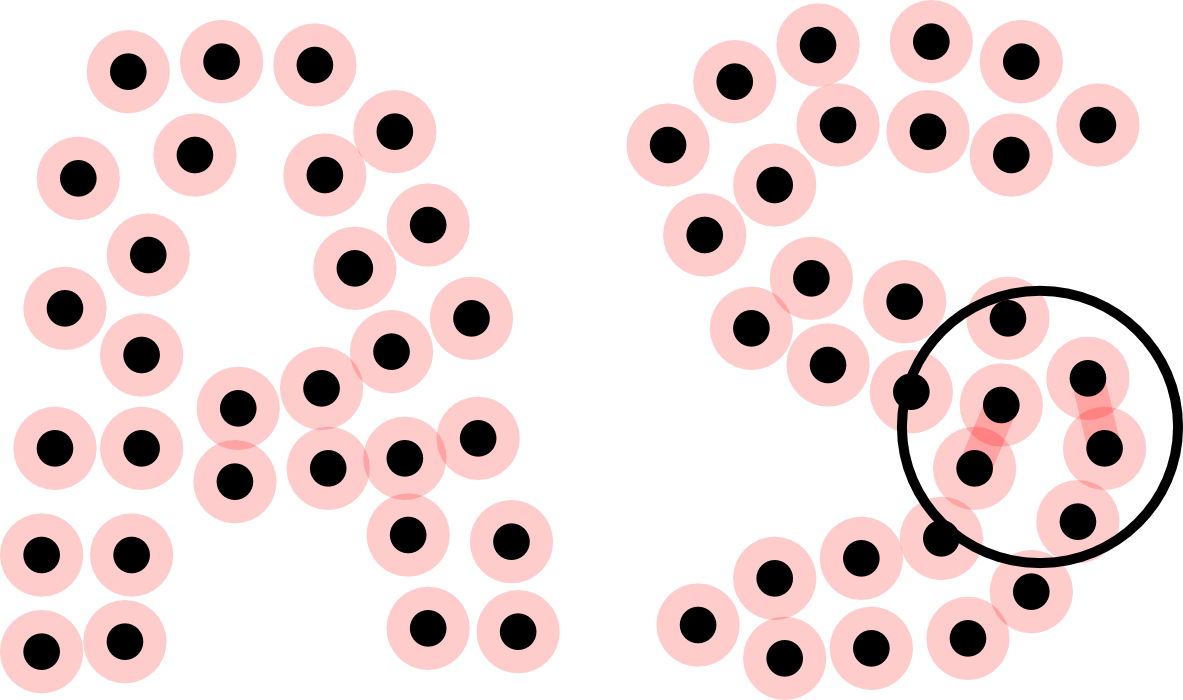
\includegraphics[scale=0.7]{../bilder/smallAS_shapeHull_closestPair.png}
	\caption{Kanten der $\alpha$-Shape verbinden dichteste Paare}
	\label{fig:shapeHull_closestPair}
\end{figure}

In Abbildung~\ref{fig:shapeHull_closestPair} ist der Bereich hervorgehoben, in welchem sich zwei dichteste Paare befinden.

Für größer werdende positive $\alpha$ existieren im Allgemeinen mehr Knoten-Paare, welche auf dem Rand einer $\alpha$-Kreisscheibe liegen. Dadurch wird die Kantenmenge größer. Die $\alpha$-Hülle entspricht derjenigen Fläche, welche nicht mehr von den $\alpha$-Kreisscheiben ausgefüllt werden kann. Punkte, welche im inneren der $\alpha$-Hülle liegen, sind nicht mehr $\alpha$-extrem und zählen damit nicht mehr zur Knotenmenge der $\alpha$-Shape.

\begin{figure}[htbp]
	\centering
	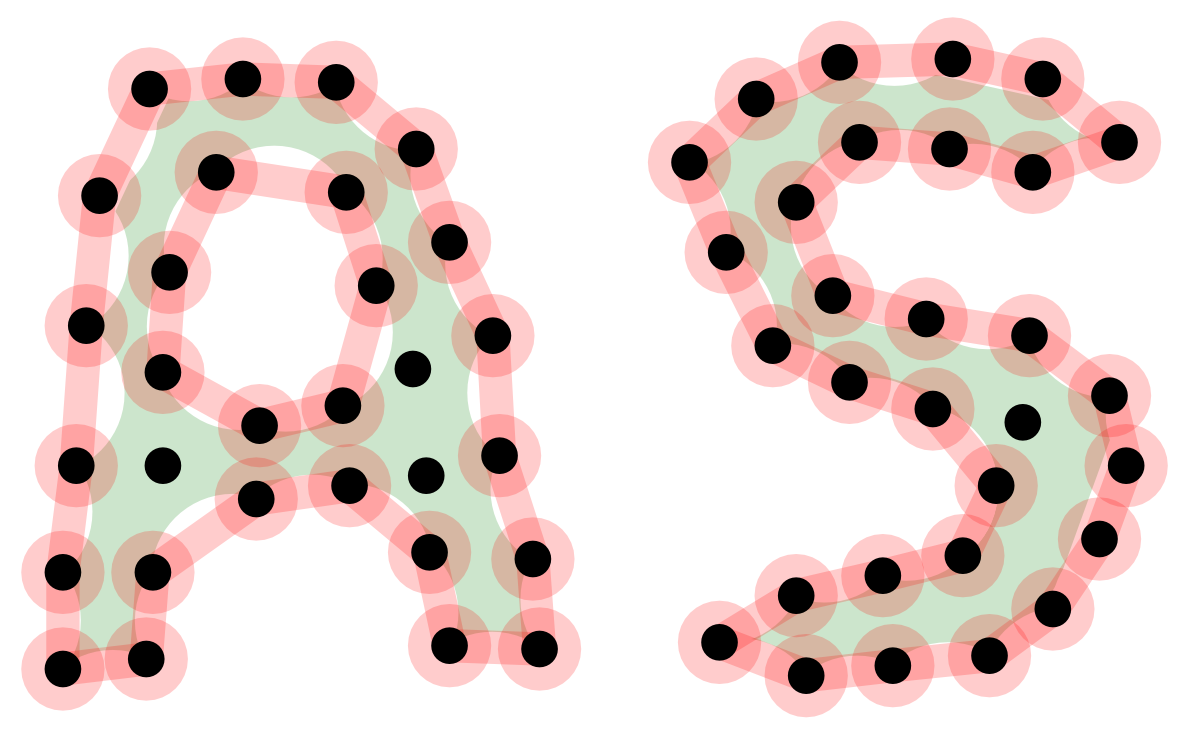
\includegraphics[scale=0.7]{../bilder/smallAS_shapeHull_positive.png}
	\caption{$\alpha$-Shape und -Hülle empfinden Gestalt sehr genau nach}
	\label{fig:shapeHull_positive}
\end{figure}

Abbildung~\ref{fig:shapeHull_positive} zeigt eine durch $\alpha$-Shape und $\alpha$-Hülle sehr genau nachempfundene Gestalt einer Punktmenge.

Variiert man $\alpha$ hin zu noch größeren Werten, so ergibt sich eine zusammenhängende $\alpha$-Shape. Einzelne Figuren werden nun durch die $\alpha$-Shape verbunden.

\begin{figure}[htbp]
	\centering
	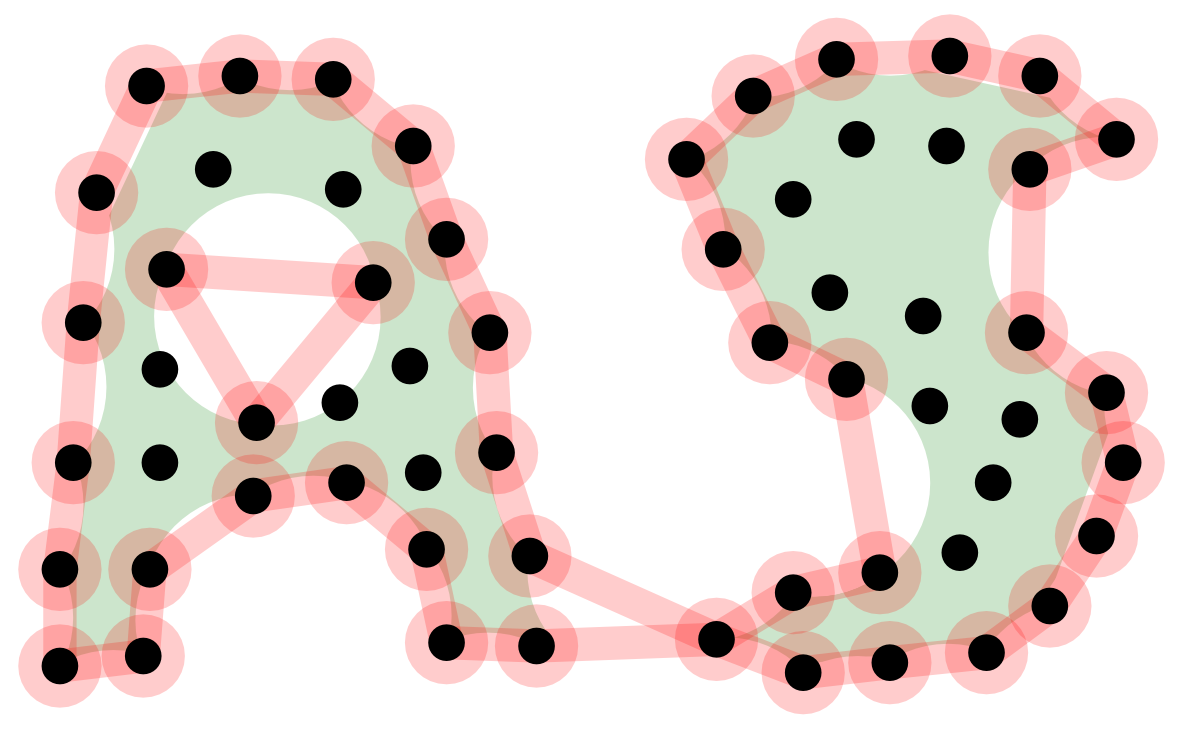
\includegraphics[scale=0.7]{../bilder/smallAS_shapeHull_connectedGraph.png}
	\caption{$\alpha$-Shape als zusammenhängender Graph}
	\label{fig:shapeHull_connectedGraph}
\end{figure}

Abbildung~\ref{fig:shapeHull_connectedGraph} zeigt eine zusammenhängende $\alpha$-Shape.

Für sehr große Werte von $\alpha$ ist nicht nur die $\alpha$-Shape ein zusammenhängender Graph, sondern auch die $\alpha$-Hülle ist eine zusammenhängende Fläche.

\begin{figure}[htbp]
	\centering
	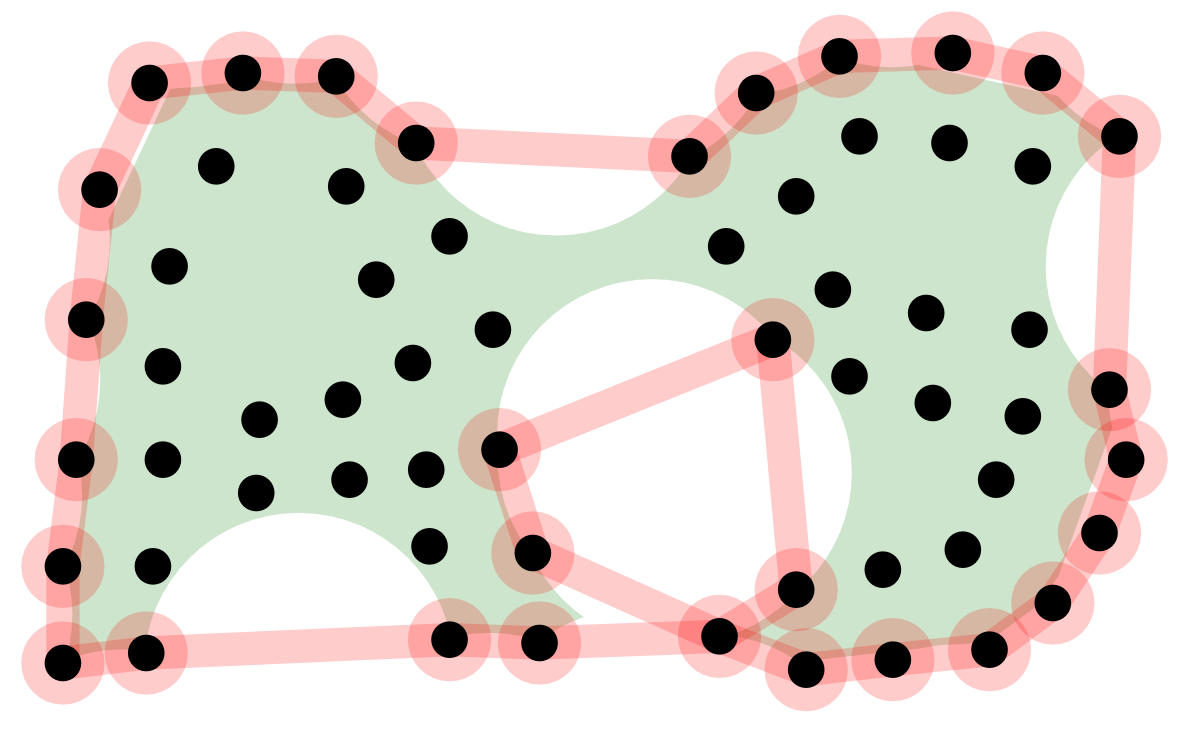
\includegraphics[scale=0.7]{../bilder/smallAS_shapeHull_connectedHull.png}
	\caption{$\alpha$-Hülle als zusammenhängende Fläche}
	\label{fig:shapeHull_connectedHull}
\end{figure}

Abbildung~\ref{fig:shapeHull_connectedHull} zeigt eine zusammenhängende $\alpha$-Hülle.

Ist $\alpha$ unendlich groß, so ist die $\alpha$-Hülle wieder gleich der konvexen Hülle.


% !TEX encoding = UTF-8 Unicode

\chapter{Eigenschaften von \boldmath{$\alpha$}-Shapes}\label{alpha_props}

Da die Menge der $\alpha$-Kreisscheiben einer Punktmenge im Allgemeinen unendlich groß ist, kann sie nicht direkt zur Bestimmung der $\alpha$-Shape verwendet werden.

In diesem Kapitel soll gezeigt werden, dass die $\alpha$-Shape ein Subgraph des Delaunay-Graphen ist. Das Shape-Spektrum ermöglicht die schnelle Identifizierung der Knoten und Kanten der $\alpha$-Shape in den Knoten und Kanten des Delaunay-Graphen. Der Delaunay-Graph und das Shape-Spektrum werden mit Hilfe des \- Voronoi-Diagramms bestimmt.

Für die folgenden Definitionen sei wieder eine Punktmenge $S$ gegeben. Die definierten Begriffe beziehen sich immer auf diese Punktmenge.

\section{Das Voronoi-Diagramm}

Das Voronoi-Diagramm von $S$ ist eine Unterteilung der Ebene in Voronoi-Zellen. Jede Zelle hat ein Zentrum, welches ein Punkt $P \in S$ ist. Ob ein Punkt $P_i$ der Ebene in einer Zelle liegt ist vom Abstand des Punktes $P_i$ zum Zentrum $P$ der Zelle abhängig. Es gibt zwei Ausprägungen des Voronoi-Diagramms. In der ersten Ausprägung ist das Kriterium, ob ein Punkt der Ebene in einer Zelle liegt, ein möglichst kleiner Abstand zu ihrem Zentrum.

\begin{defin}
Das \emph{Voronoi-Diagramm \- der \- Punkte \- mit \- minimalem \- Abstand}, \- $VD_{\min}(S)$, \- ist eine vollständige Unterteilung der Ebene in Teilflächen, den sogenannten Voronoi-Zellen. Für jeden Punkt $P \in S$ existiert eine eindeutige \emph{Voronoi-Zelle der Punkte mit minimalem Abstand} $VC_{\min}(P)$. $P$ ist das Zentrum dieser Zelle. Der Abstand jedes Punktes $P_i \in VC_{\min}(P)$ zu $P$ ist kleiner oder gleich dem Abstand von $P_i$ zu einem anderen Zentrum.
\end{defin}

Das Voronoi-Diagramm der Punkte mit minimalem Abstand wird im Folgenden auch kurz als Minimum-Voronoi-Diagramm und die zugehörige Voronoi-Zelle als Minimum-Voronoi-Zelle bezeichnet.

In der zweiten Ausprägung des Voronoi-Diagramms ist das Kriterium, ob ein Punkt der Ebene zu einer Zelle gehört, ein möglichst großer Abstand zu ihrem Zentrum.

\begin{defin}
Das \emph{Voronoi-Diagramm \- der \- Punkte \- mit \- maximalem \- Abstand}, \- $VD_{\max}(S)$, \- ist eine vollständige Unterteilung der Ebene in Voronoi-Zellen. Für jeden Punkt $P \in S$, welcher auf dem Rand der konvexen Hülle liegt, existiert eine eindeutige \emph{Voronoi-Zelle der Punkte mit maximalem Abstand} $VC_{\max}(P)$. $P$ ist das Zentrum dieser Zelle. Der Abstand jedes Punktes $P_i \in VC_{\max}(P)$ zu $P$ ist größer oder gleich dem Abstand von $P_i$ zu einem anderen Zentrum.
\end{defin}

Das Voronoi-Diagramm der Punkte mit maximalem Abstand wird im Folgenden auch kurz als Maximum-Voronoi-Diagramm und die zugehörige Voronoi-Zelle als Maximum-Voronoi-Zelle bezeichnet.

\begin{figure}[htbp]
	\centering
	\subfloat[Minimum-Voronoi-Diagramm und -Zelle\label{fig:voronoi_min}]
		{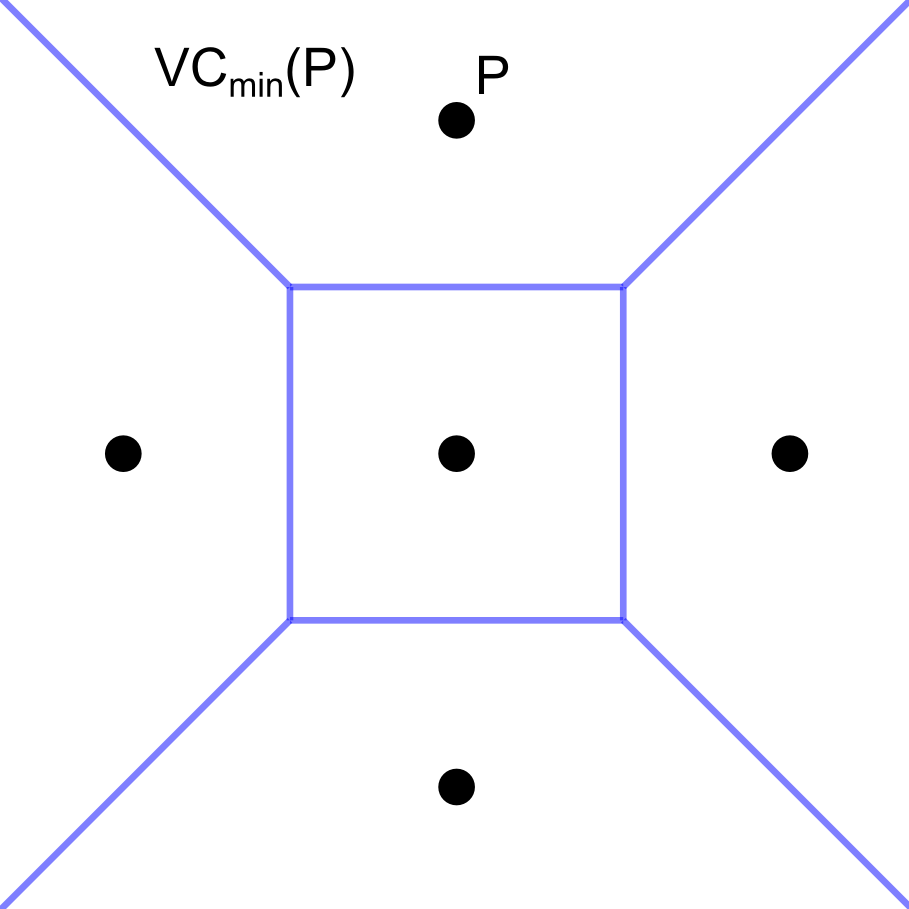
\includegraphics[scale=0.7]{../bilder/voronoi_min.png}}
	\hspace{2cm}
	\subfloat[Maximum-Voronoi-Diagramm und -Zelle\label{fig:voronoi_max}]
		{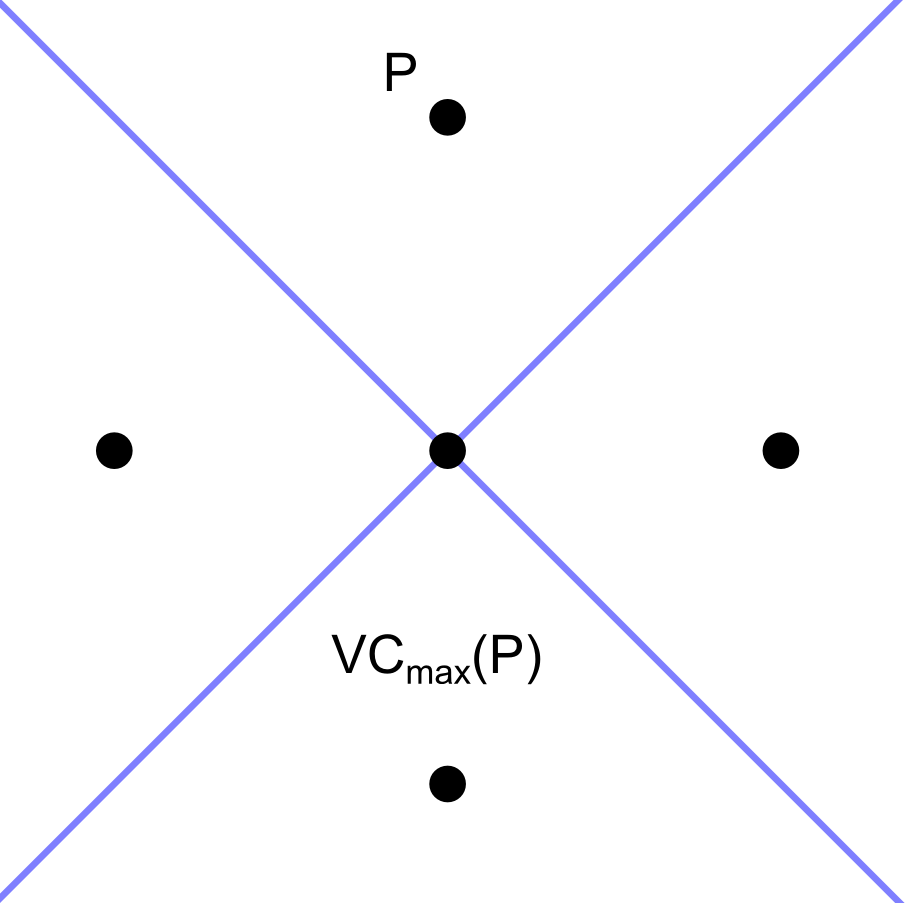
\includegraphics[scale=0.7]{../bilder/voronoi_max.png}}
	\caption{Voronoi-Diagramme und -Zellen}
	\label{fig:voronoi}	
\end{figure}

Abbildung~\ref{fig:voronoi} zeigt das Minimum- und Maximum-Voronoi-Diagramm einer einfachen Punktmenge sowie je eine beschriftete Zelle und ihr Zentrum.

\begin{eigen}
Sei $B$ die Menge der Strecken, Strahlen und Geraden, welche die Voronoi-Zellen eines Voronoi-Diagramms begrenzen. Jedes $b \in B$ liegt auf der Streckenhalbierenden zwischen den Zentren $P_1$ und $P_2$ zweier Voronoi-Zellen und trennt diese voneinander. Der Abstand eines Punktes $P_b \in b$ zu $P_1$ ist daher gleich dem Abstand von $P_b$ zu $P_2$ und $P_b$ liegt in beiden Voronoi-Zellen.
\end{eigen}

Das Voronoi-Diagramm ist eine Einbettung des Voronoi-Graphen in die Ebene. Der Voronoi-Graph kann über das Voronoi-Diagramm definiert werden.

\begin{defin}
Gegeben sei ein Voronoi-Diagramm. Die Strecken, Strahlen und Geraden, welche die Voronoi-Zellen des Voronoi-Diagramms begrenzen, sind die \emph{Kanten des Voronoi-Graphen}. Die Endpunkte der Strecken und die Ursprünge der Strahlen sind die \emph{Knoten des Voronoi-Graphen}. Zusätzlich existiert ein virtueller Knoten im Unendlichen.\\
Die Strecken verbinden ihre Endpunkte. Die Strahlen verbinden ihren Ursprung mit dem virtuellen Knoten. Die Geraden verbinden den virtuellen Knoten mit sich selbst.
\end{defin}

\begin{figure}[htbp]
	\centering
	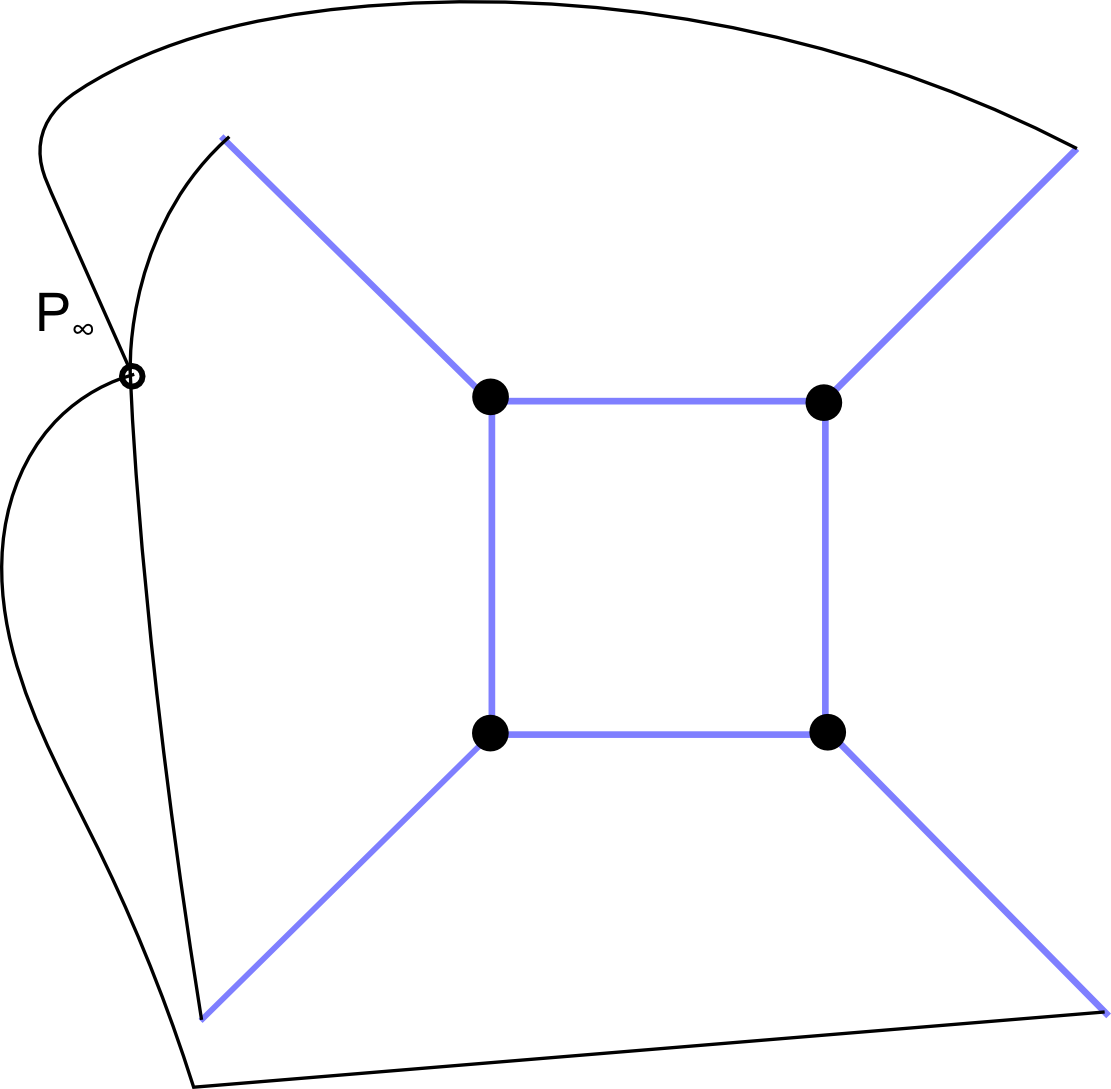
\includegraphics[scale=1.0]{../bilder/voronoiGraph_min.png}
	\caption{Voronoi-Graph mit dem virtuellen Knoten}
	\label{fig:voronoiGraph_min}
\end{figure}

Abbildung~\ref{fig:voronoiGraph_min} zeigt das Minimum-Voronoi-Diagramm aus Abbildung~\ref{fig:voronoi_min} mit dem virtuellen Knoten $P_{\infty}$ und seinen Verbindungen.

\begin{eigen}
Die Kanten des Voronoi-Diagramms kreuzen sich nicht. Damit ist der Voronoi-Graph ein planarer Graph.
\end{eigen}

\section{Der Delaunay-Graph}

Der Delaunay-Graph von $S$ ist ein dualer Graph zum Voronoi-Diagramm von $S$. Für seine Definition wird zuerst definiert, wann zwei Voronoi-Zellen benachbart sind.

\begin{defin}
Gegeben sei ein Voronoi-Diagramm. Zwei \emph{Voronoi-Zellen} sind genau dann \emph{benachbart}, wenn sie eine gemeinsame Kante $b$ besitzen.
\end{defin}

Damit lässt sich der Delaunay-Graph wie folgt definieren.

\begin{defin}
Gegeben sei das Voronoi-Diagramm von $S$. Der \emph{Delaunay-Graph von $S$} ist der Graph, dessen Knoten die Zentren der Voronoi-Zellen sind und dessen Kanten die Zentren benachbarter Voronoi-Zellen verbinden.
\end{defin}

Auch für den Delaunay-Graphen existieren zwei Ausprägungen. Je nachdem aus welchem Voronoi-Diagramm der Graph abgeleitet ist, spricht man vom Delaunay-Graphen der Punkte mit minimalem Abstand, $DG_{\min}(S)$, oder maximalem Abstand, $DG_{\max}(S)$.

Im Folgenden werden auch die Bezeichnungen Minimum-Delaunay-Graph und Maximum-Delaunay-Graph verwendet.

\begin{figure}[htbp]
	\centering
	\subfloat[Minimum-Voronoi-Diagramm und -Delaunay-Graph\label{fig:voronoiDelaunay_min}]
		{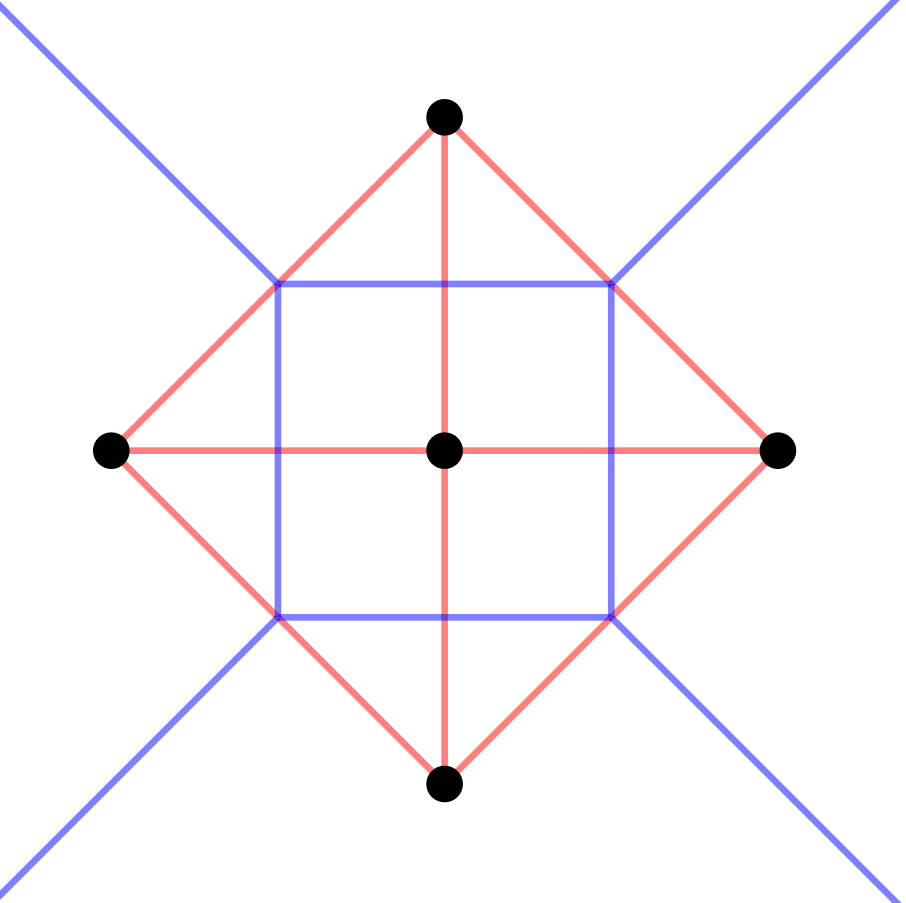
\includegraphics[scale=0.7]{../bilder/voronoiDelaunay_min.png}}
	\hspace{2cm}
	\subfloat[Maximum-Voronoi-Diagramm und -Delaunay-Graph\label{fig:voronoiDelaunay_max}]
		{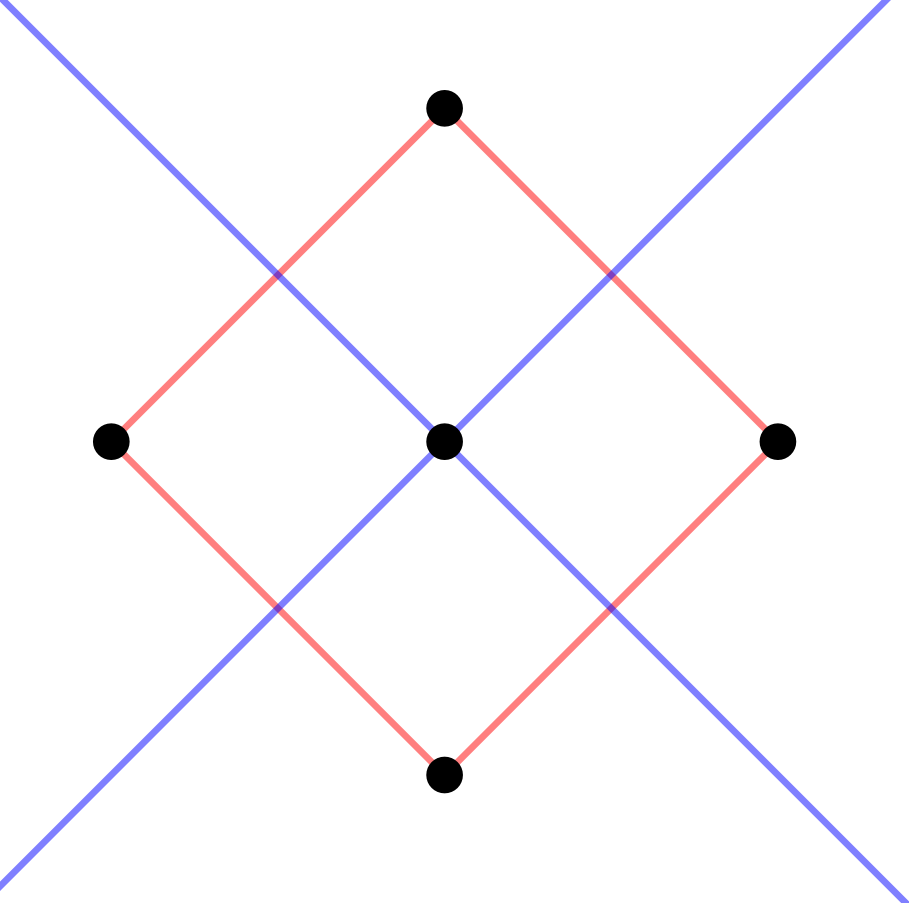
\includegraphics[scale=0.7]{../bilder/voronoiDelaunay_max.png}}
	\caption{Voronoi-Diagramme und Delaunay-Graphen}
	\label{fig:voronoiDelaunay}	
\end{figure}

Abbildung~\ref{fig:voronoiDelaunay} zeigt Minimum- und Maximum-Voronoi-Diagramme sowie die zugehörigen Delaunay-Graphen einer einfachen Punktmenge.

\section[Die $\alpha$-Shape als Subgraph des Delaunay-Graphen]{Die \boldmath{$\alpha$}-Shape als Subgraph des Delaunay-Graphen}

Die $\alpha$-Shape ist ein Subgraph des Delaunay-Graphen. Folgende Eigenschaften des Voronoi-Diagramms und des Delaunay-Graphen sind für den Beweis dafür wichtig. Alle Aussagen gelten sowohl für positve $\alpha$-Shape und -Kreisscheiben in Bezug auf Minimum-Voronoi-Diagramm und -Delaunay-Graph als auch für negative $\alpha$-Shape und -Kreisscheiben in Bezug auf Maximum-Voronoi-Diagramm und -Delaunay-Graph.

\begin{eigen}\label{eigen_alphaExtreme_VD}
Gegeben sei das Voronoi-Diagramm von $S$. Sei eine beliebige Voronoi-Zelle mit einem Zentrum $P \in S$ gegeben. Diese Zelle ist der Ort der Mittelpunkte $P_C$ derjenigen $\alpha$-Kreisscheiben, welche $P$ auf ihrem Rand haben. Der Radius einer solchen $\alpha$-Kreisscheibe ist gleich dem Abstand von $P_C$ zu $P$. Kein anderer Ort kann Mittelpunkt einer solchen $\alpha$-Kreisscheibe sein.
\end{eigen}

\begin{figure}[htbp]
	\centering
	\subfloat[Positive $\alpha$-Kreisscheibe und Minimum-Voronoi-Zelle\label{fig:alphaExtreme_VDmin}]
		{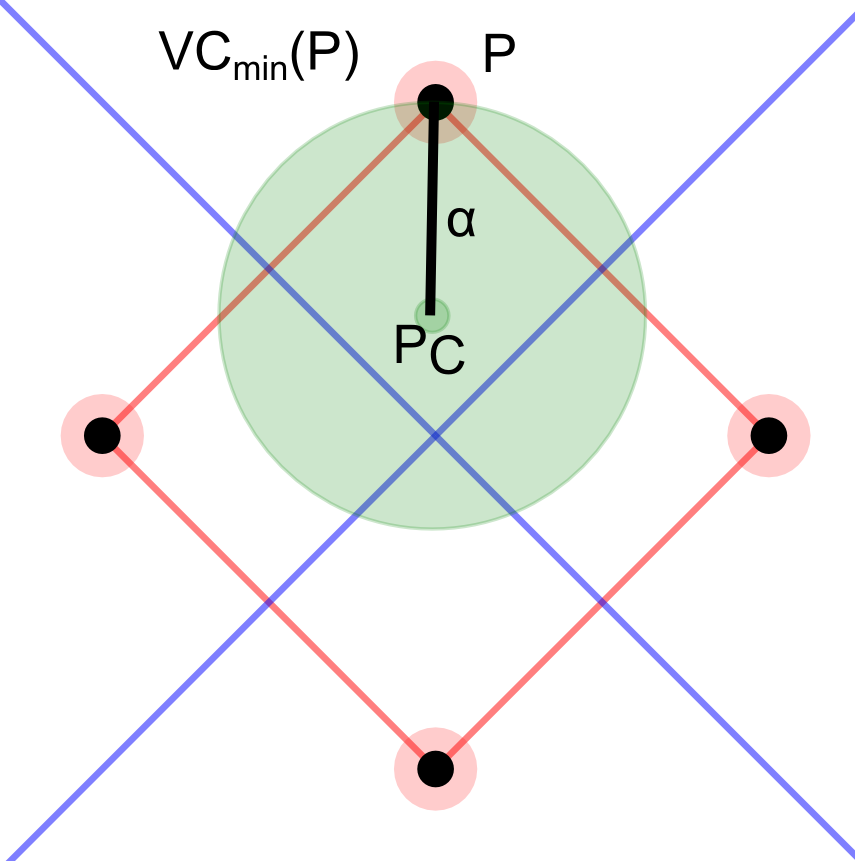
\includegraphics[scale=0.7]{../bilder/alphaExtreme_VDmin.png}}
	\hspace{2cm}
	\subfloat[Negative $\alpha$-Kreisscheibe und Maximum-Voronoi-Zelle\label{fig:alphaExtreme_VDmax}]
		{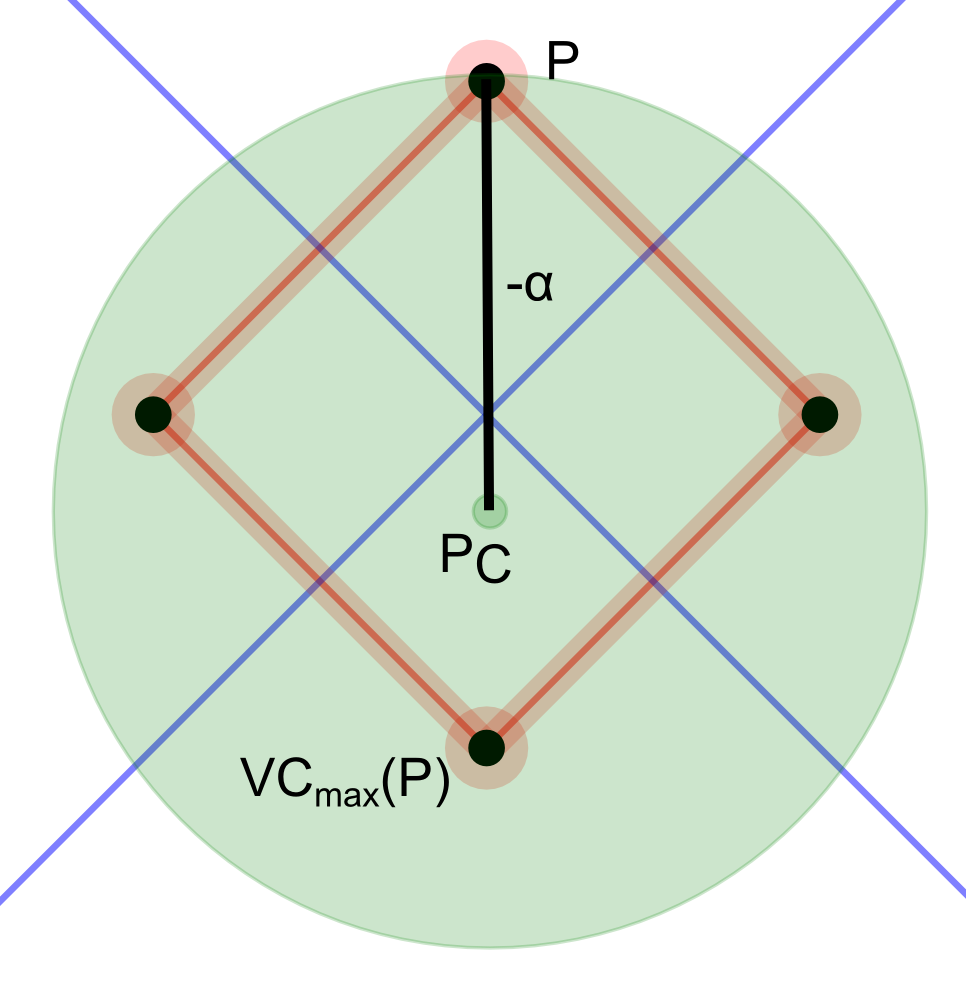
\includegraphics[scale=0.7]{../bilder/alphaExtreme_VDmax.png}}
	\caption{$\alpha$-Kreisscheiben mit Mittelpunkten in Voronoi-Zellen}
	\label{fig:alphaExtreme_VD}	
\end{figure}

Abbildung~\ref{fig:alphaExtreme_VD} stellt Beispiele zu Eigenschaft \ref{eigen_alphaExtreme_VD} dar.

\begin{eigen}\label{eigen_alphaNeighbours_VD}
Gegeben sei das Voronoi-Diagramm von $S$. Sei $b$ die Kante zwischen den Voronoi-Zellen mit den Zentren $P_1,P_2 \in S$. Die Kante $b$ ist der Ort der Mittelpunkte $P_C$ derjenigen $\alpha$-Kreisscheiben, auf deren Rand $P_1$ und $P_2$ direkt benachbart sind. Der Radius einer solchen $\alpha$-Kreisscheibe ist gleich dem Abstand von $P_1$ und $P_2$ zu $P_C$. Kein anderer Ort kann Mittelpunkt einer solchen Kreisscheibe sein.
\end{eigen}

\begin{figure}[htbp]
	\centering
	\subfloat[Positive $\alpha$-Kreisscheibe und Kante zwischen Minimum-Voronoi-Zellen\label{fig:alphaNeighbours_VDmin}]
		{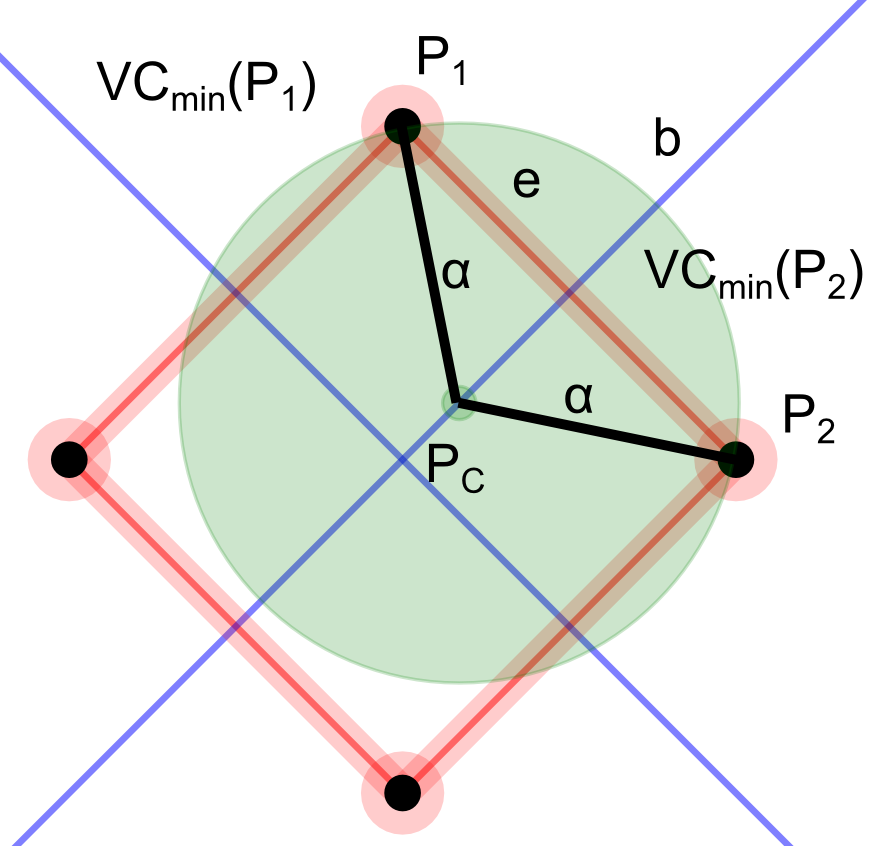
\includegraphics[scale=0.7]{../bilder/alphaNeighbours_VDmin.png}}
	\hspace{2cm}
	\subfloat[Negative $\alpha$-Kreisscheibe und Kante zwischen Maximum-Voronoi-Zellen\label{fig:alphaNeighbours_VDmax}]
		{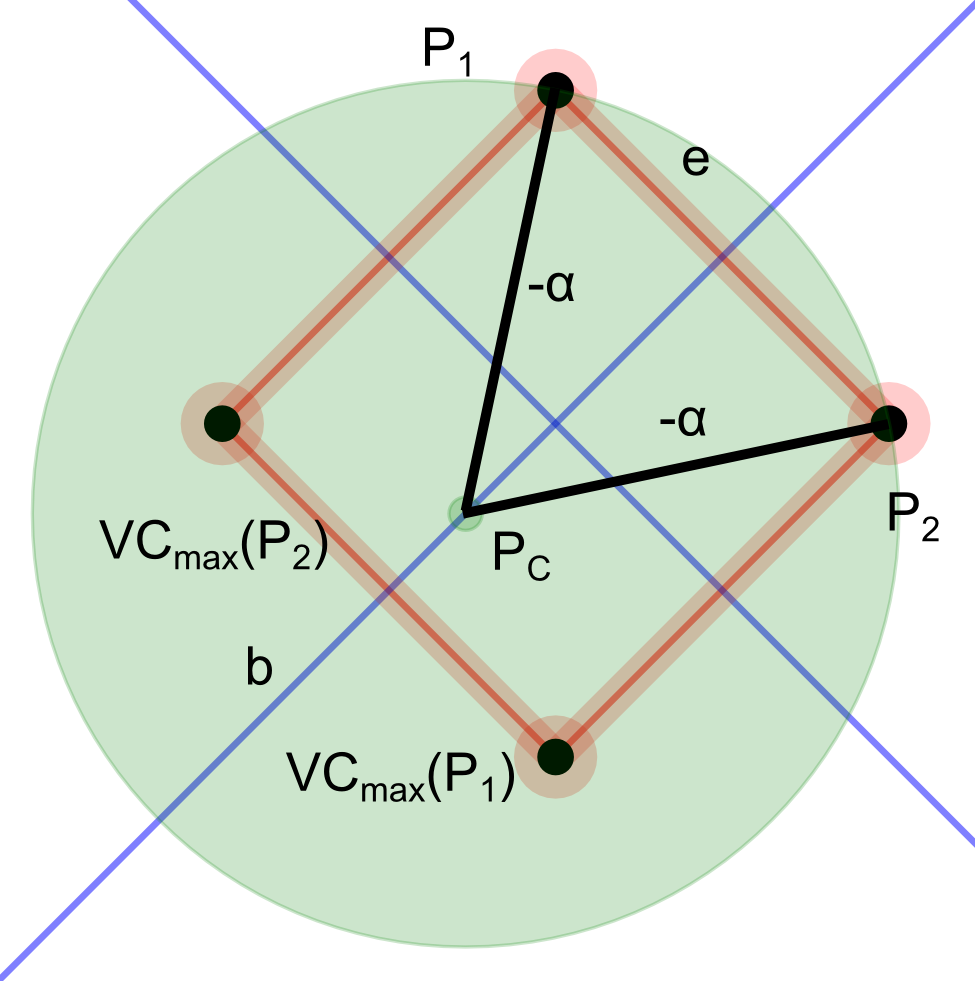
\includegraphics[scale=0.7]{../bilder/alphaNeighbours_VDmax.png}}
	\caption{$\alpha$-Kreisscheiben mit Mittelpunkten auf der gemeinsamen Kante zweier Voronoi-Zellen}
	\label{fig:alphaNeighbours_VD}	
\end{figure}

Abbildung~\ref{fig:alphaNeighbours_VD} stellt Beispiele zu Eigenschaft \ref{eigen_alphaNeighbours_VD} dar.

Hiermit sollen nun folgende Aussagen bewiesen werden.

\begin{lemma}\label{lemma:alphaSubgraph}
Die $\alpha$-Shape von $S$ ist ein Subgraph des Delaunay-Graphen von $S$.
\end{lemma}

Um dies zu Beweisen, wird die Aussage in folgende Teilaussagen zerlegt:

\begin{lemma}\label{lemma:knotenAlphaDelaunay}
Jeder Knoten der $\alpha$-Shape von $S$ ist auch ein Knoten des Delaunay-Graphen von $S$.
\end{lemma}

\begin{proof}[Beweis zu Lemma \ref{lemma:knotenAlphaDelaunay}]
Sei $P \in S$ ein Knoten der $\alpha$-Shape von $S$. Daraus folgt, dass $P$ auf dem Rand mindestens einer $\alpha$-Kreisscheibe liegt. Der einzig mögliche Ort für Mittelpunkte $P_C$ solcher Kreisscheiben ist diejenige Voronoi-Zelle, welche $P$ als Zentrum hat. Da jedes Zentrum einer Voronoi-Zelle einem Knoten im Delaunay-Graphen enstpricht, ist $P$ auch ein Knoten des Delaunay-Graphen von $S$.
\end{proof}

\begin{lemma}\label{lemma:kanteAlphaDelaunay}
Jede Kante der $\alpha$-Shape von $S$ ist auch eine Kante des Delaunay-Graphen von $S$.
\end{lemma}

\begin{proof}[Beweis zu Lemma \ref{lemma:kanteAlphaDelaunay}]
Sei $e$ eine Kante der $\alpha$-Shape von $S$. Daraus folgt, dass $e$ zwei $\alpha$-Nachbarn $P_1,P_2 \in S$ verbindet. $\alpha$-Nachbarn sind auf dem Rand mindestens einer $\alpha$-Kreisscheibe direkt benachbart. Der einzig mögliche Ort für Mittelpunkte $P_C$ solcher Kreisscheiben ist die Voronoi-Kante $b$ zwischen den beiden Voronoi-Zellen, welche $P_1$ und $P_2$ als Zentrum haben. Da mindestens ein $P_C$ existiert muss auch $b$ existieren. Da $b$ existiert, sind die Voronoi-Zellen benachbart und $e$ ist damit auch eine Kante im Delaunay-Graphen von $S$.
\end{proof}

\begin{lemma}\label{lemma:knotenDelaunayAlpha}
Für jeden Knoten des Delaunay-Graphen von $S$ existiert mindestens ein $\alpha$, für welches der Knoten auch ein Knoten der $\alpha$-Shape von $S$ ist.
\end{lemma}

\begin{proof}[Beweis zu Lemma \ref{lemma:knotenDelaunayAlpha}]
Sei $P \in S$ ein Knoten des Delaunay-Graphen von $S$. Daraus folgt, dass $P \in S$ das Zentrum einer Voronoi-Zelle ist. Sei $P_C$ ein Punkt innerhalb dieser Voronoi-Zelle. Sei der Betrag von $\alpha$ gleich dem Abstand von $P_C$ zu $P$. Für ein solches $\alpha$ liegt $P$ auf dem Rand der $\alpha$-Kreisscheibe mit Mittelpunkt $P_C$ und ist somit $\alpha$-extrem. Somit ist $P$ auch ein Knoten der $\alpha$-Shape von $S$.
\end{proof}

\begin{lemma}\label{lemma:kanteDelaunayAlpha}
Für jede Kante des Delaunay-Graphen von $S$ existiert mindestens ein $\alpha$, für welches die Kante auch eine Kante der $\alpha$-Shape von $S$ ist.
\end{lemma}

\begin{proof}[Beweis zu Lemma \ref{lemma:kanteDelaunayAlpha}]
Sei $e$ eine Kante des Delaunay-Graphen von $S$. Die Kante verbindet die Zentren $P_1,P_2 \in S$ zweier benachbarter Voronoi-Zellen. Sei $b$ die Voronoi-Kante zwischen diesen Voronoi-Zellen. Sei $P_C$ ein beliebiger Punkt auf $b$. Der Betrag von $\alpha$ sei gleich dem Abstand von $P_C$ zu $P_1$ und $P_2$. Für ein solches $\alpha$ sind $P_1$ und $P_2$ direkt auf dem Rand der $\alpha$-Kreisscheibe mit Mittelpunkt $P_C$ benachbart und sind somit $\alpha$-Nachbarn. Somit ist $e$ auch eine Kante der $\alpha$-Shape von $S$.
\end{proof}

\begin{proof}[Beweis zu Lemma \ref{lemma:alphaSubgraph}]
Aus der Richtigkeit der Lemmata \ref{lemma:knotenAlphaDelaunay}, \ref{lemma:kanteAlphaDelaunay}, \ref{lemma:knotenDelaunayAlpha} und \ref{lemma:kanteDelaunayAlpha} folgt die Richtigkeit von Lemma \ref{lemma:alphaSubgraph}.
\end{proof}

\section{Das Shape-Spektrum}

Das Shape-Spektrum wird zur Konstruktion einer $\alpha$-Shape aus einem Delaunay-Graphen verwendet werden. Es ist folgendermaßen definiert.

\begin{defin}
Das \emph{positive Shape-Spektrum}, $Sp^+$, \emph{eines Knotens bzw. einer Kante des Minimum-Delaunay-Graphen von $S$} ist die Menge aller positiven $\alpha$, für welche der Knoten bzw. die Kante ein Teil der $\alpha$-Shape von $S$ ist.
Das \emph{negative Shape-Spektrum}, $Sp^-$, \emph{eines Knotens bzw. einer Kante eines Maximum-Delaunay-Graphen von $S$} ist die Menge aller negativen $\alpha$, für welche der Knoten bzw. die Kante ein Teil der $\alpha$-Shape von $S$ ist.
\end{defin}

Folgende Eigenschaften des Voronoi-Diagramms können für die Bestimmung der Shape-Spektren verwendet werden.

\begin{eigen}
Die Zentren der Zellen des Minimum-Voronoi-Diagramms von $S$ liegen innerhalb ihrer Zellen. Die Zentren der Zellen des Maximum-Voronoi-Diagramms von $S$ liegen, für $\mid S \mid > 1$, außerhalb ihrer Zellen. Für $\mid S \mid = 1$ besteht das Voronoi-Diagramm genau aus einer Zelle, welche die gesamte Ebene einnimmt. Das Zentrum dieser Zelle liegt in der Ebene und damit auch in der Zelle. 
\end{eigen}

\begin{eigen}
Sei ein Voronoi-Diagramm von $S$ gegeben. Sei $P \in S$ ein Punkt, welcher nicht auf dem Rand der konvexen Hülle von $S$ liegt. Die Voronoi-Zelle mit dem Zentrum $P$ ist eine endliche Teilfläche der Ebene.
\end{eigen}

\begin{eigen}
Sei ein Voronoi-Diagramm von $S$ gegeben. Sei $P \in S$ ein Punkt, welcher auf dem Rand der konvexen Hülle von $S$ liegt. Die Voronoi-Zelle mit dem Zentrum $P$ ist eine unendliche Teilfläche der Ebene.
\end{eigen}

\begin{eigen}
Sei ein Voronoi-Diagramm von $S$ gegeben. Seien $P_1,P_2 \in S$ zwei Punkte, welche nicht direkt auf dem Rand der konvexen Hülle von $S$ benachbart sind. Die Kante zwischen den Voronoi-Zellen mit den Zentren $P_1$ und $P_2$ ist eine Strecke.
\end{eigen}

\begin{eigen}
Sei ein Voronoi-Diagramm von $S$ gegeben. Seien $P_1,P_2 \in S$ zwei Punkte, welche direkt auf dem Rand der konvexen Hülle von $S$ benachbart sind. Die Kante zwischen den Voronoi-Zellen mit den Zentren $P_1$ und $P_2$ ist ein Strahl oder eine Gerade.
\end{eigen}

Mit diesen Eigenschaften lassen sich die Shape-Spektren bestimmen.

\begin{lemma}\label{lemma:alphaExtreme_VDmin_alphaMax}
Sei $P \in S$ ein Knoten des Minimum-Delaunay-Graphen von $S$, welcher nicht auf dem Rand der konvexen Hülle von $S$ liegt. Dann gilt $Sp^+(P) = (0, \alpha_{\max}]$. $\alpha_{\max}$ ist der maximale Abstand von $P$ zum Rand seiner Voronoi-Zelle. 
\end{lemma}

\begin{figure}[htbp]
	\centering
	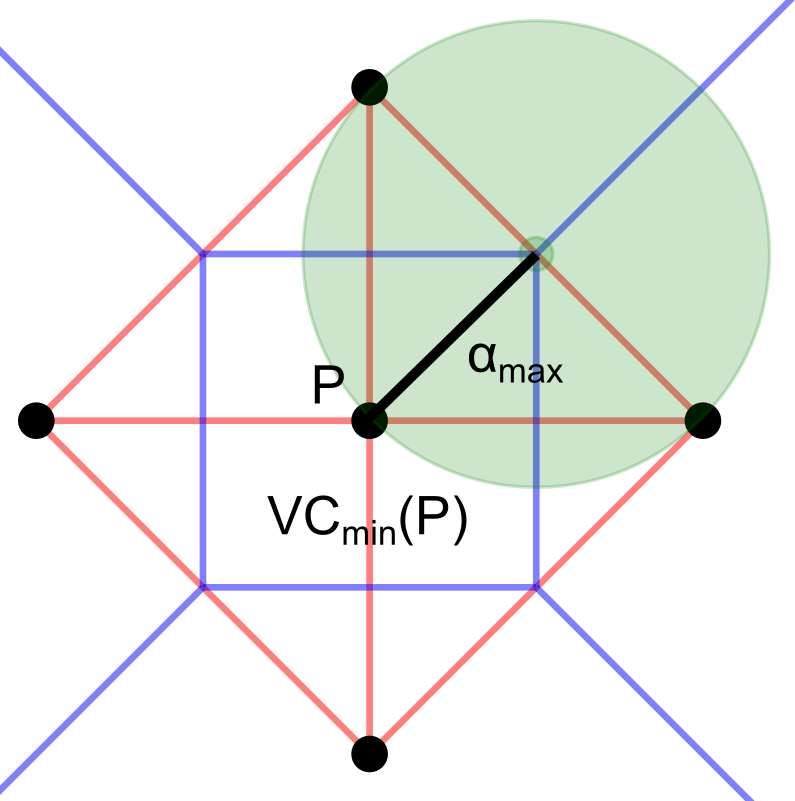
\includegraphics[scale=0.7]{../bilder/alphaExtreme_VDmin_alphaMax.png}
	\caption{$\alpha_{\max}$ für einen Knoten $P$ aus $DG_{\min}$, welcher nicht auf dem Rand der konvexen Hülle liegt}
	\label{fig:alphaExtreme_VDmin_alphaMax}
\end{figure}

Abbildung~\ref{fig:alphaExtreme_VDmin_alphaMax} zeigt ein Beispiel für die in Lemma \ref{lemma:alphaExtreme_VDmin_alphaMax} geschilderte Situation.

\begin{proof}[Beweis zu Lemma \ref{lemma:alphaExtreme_VDmin_alphaMax}]
Sei das Minimum-Voronoi-Diagramm von $S$ gegeben. Die Voronoi-Zelle mit Zentrum $P \in S$ ist der einzige Ort für Mittelpunkte von positiven $\alpha$-Kreisscheiben, welche $P$ auf ihrem Rand haben. Der Radius einer solchen $\alpha$-Kreisscheibe kann beliebig klein sein, da $P$ in seiner Voronoi-Zelle liegt. Der Radius ist nach oben begrenzt, da die Voronoi-Zellen von Punkten, welche nicht auf dem Rand der konvexen Hülle liegen, endliche Teilflächen der Ebene sind.
\end{proof}

\begin{lemma}\label{lemma:alphaExtreme_VDmin_Konvex}
Sei $P \in S$ ein Knoten des Minimum-Delaunay-Graphen von $S$, welcher auf dem Rand der konvexen Hülle von $S$ liegt. Dann gilt $Sp^+(P) = (0, \infty)$.
\end{lemma}

\begin{figure}[htbp]
	\centering
	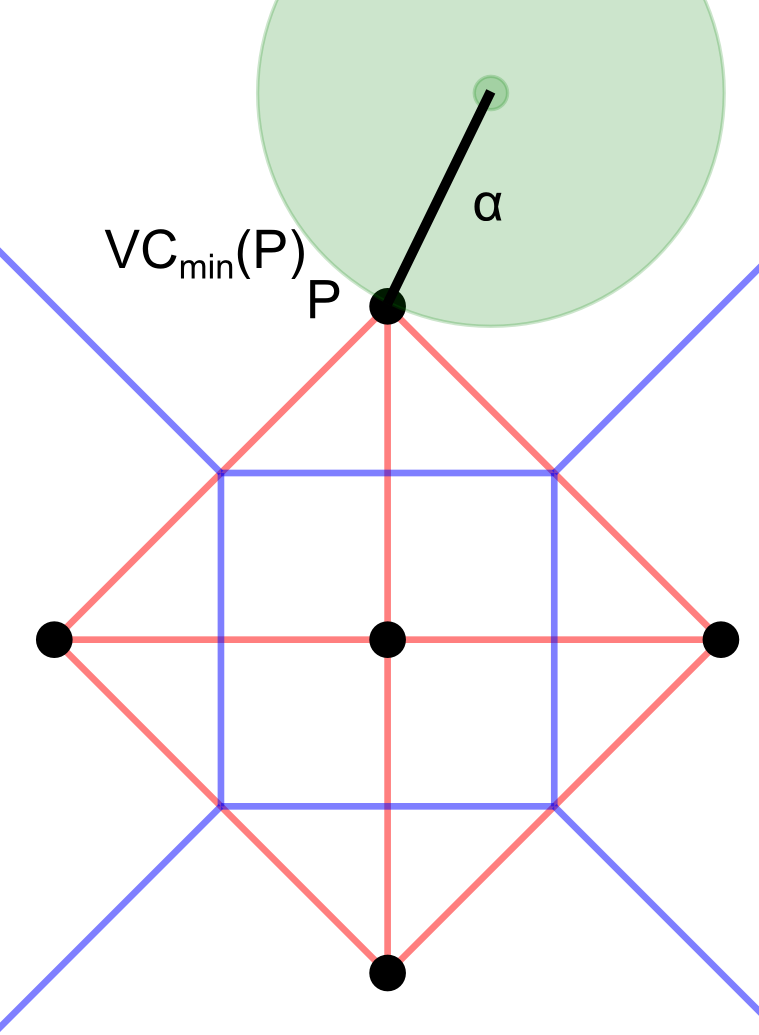
\includegraphics[scale=0.7]{../bilder/alphaExtreme_VDmin_Konvex.png}
	\caption{Beliebiges $\alpha$ für einen Knoten $P$ aus $DG_{\min}$, welcher auf dem Rand der konvexen Hülle liegt}
	\label{fig:alphaExtreme_VDmin_Konvex}
\end{figure}

Abbildung~\ref{fig:alphaExtreme_VDmin_Konvex} zeigt ein Beispiel für die in Lemma \ref{lemma:alphaExtreme_VDmin_Konvex} geschilderte Situation.

\begin{proof}[Beweis zu Lemma \ref{lemma:alphaExtreme_VDmin_Konvex}]
Sei das Minimum-Voronoi-Diagramm von $S$ gegeben. Die Voronoi-Zelle mit Zentrum $P \in S$ ist der einzige Ort für Mittelpunkte von positiven $\alpha$-Kreisscheiben, welche $P$ auf ihrem Rand haben. Der Radius einer solchen $\alpha$-Kreisscheibe kann beliebig klein sein, da $P$ in seiner Voronoi-Zelle liegt. Der Radius ist nicht nach oben begrenzt, da die Voronoi-Zellen von Punkten, welche auf dem Rand der konvexen Hülle liegen, unendliche Teilflächen der Ebene sind.
\end{proof}

\begin{lemma}\label{lemma:alphaExtreme_VDmax_alphaMax}
Sei $P \in S$ ein Knoten des Maximum-Delaunay-Graphen von $S$. Dann gilt $Sp^-(P) = (-\infty, \alpha_{\max}]$. $\alpha_{\max}$ ist die Negation des minimalen Abstands von $P$ zum Rand seiner Voronoi-Zelle. 
\end{lemma}

\begin{figure}[htbp]
	\centering
	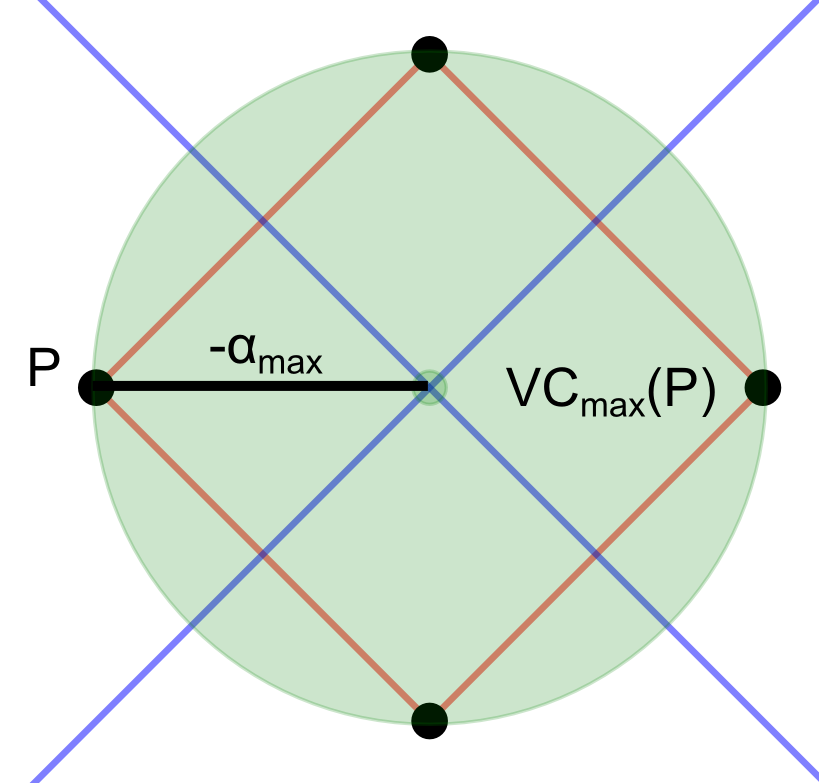
\includegraphics[scale=0.7]{../bilder/alphaExtreme_VDmax_alphaMax.png}
	\caption{$\alpha_{\max}$ für einen Knoten $P$ aus $DG_{\max}$}
	\label{fig:alphaExtreme_VDmax_alphaMax}
\end{figure}

Abbildung~\ref{fig:alphaExtreme_VDmax_alphaMax} zeigt ein Beispiel für die in Lemma \ref{lemma:alphaExtreme_VDmax_alphaMax} geschilderte Situation.

\begin{proof}[Beweis zu Lemma \ref{lemma:alphaExtreme_VDmax_alphaMax}]
Sei das Maximum-Voronoi-Diagramm von $S$ gegeben. Die Voronoi-Zelle mit Zentrum $P \in S$ ist der einzige Ort für Mittelpunkte von negativen $\alpha$-Kreisscheiben, welche $P$ auf ihrem Rand haben. Der Radius einer solchen $\alpha$-Kreisscheibe muss mindestens gleich dem minimalen Abstand von $P$ zu seiner Voronoi-Zelle sein, da $P$ nicht in seiner Voronoi-Zelle liegt. Der Radius ist nicht nach oben begrenzt, da Maximum-Voronoi-Zellen unendliche Teilflächen der Ebene sind, weil ihre Zentren immer auf dem Rand der konvexen Hülle liegen.
\end{proof}

\begin{lemma}\label{lemma:alphaNeighbours_VDmin_alphaMinMax}
Sei $e=(P_1,P_2)$ eine Kante des Minimum-Delaunay-Graphen von $S$. Seien $P_1,P_2 \in S$ nicht direkt auf dem Rand der konvexen Hülle von $S$ benachbart. Sei $b$ die Voronoi-Kante zwischen den Voronoi-Zellen mit den Zentren $P_1$ und $P_2$. Dann gilt $Sp^+(e) = [\alpha_{\min}, \alpha_{\max}]$. $\alpha_{\min}$ ist der minimale und $\alpha_{\max}$ der maximale Abstand von $P_1$ und $P_2$ zu $b$.
\end{lemma}

\begin{figure}[htbp]
	\centering
	\subfloat[$\alpha_{\min}$ für Kante $e$ aus $DG_{\min}$, deren Knoten nicht auf dem Rand der konvexen Hülle benachbart sind\label{fig:alphaNeighbours_VDmin_alphaMin}]
		{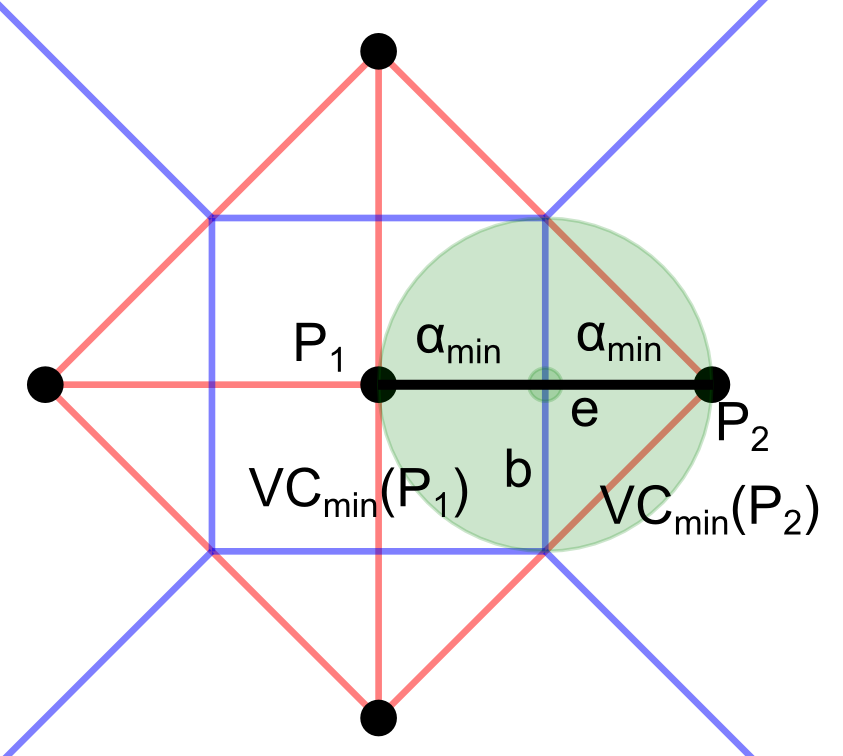
\includegraphics[scale=0.7]{../bilder/alphaNeighbours_VDmin_alphaMin.png}}
	\hspace{2cm}
	\subfloat[$\alpha_{\max}$ für Kante $e$ aus $DG_{\min}$, deren Knoten nicht auf dem Rand der konvexen Hülle benachbart sind\label{fig:alphaNeighbours_VDmin_alphaMax}]
		{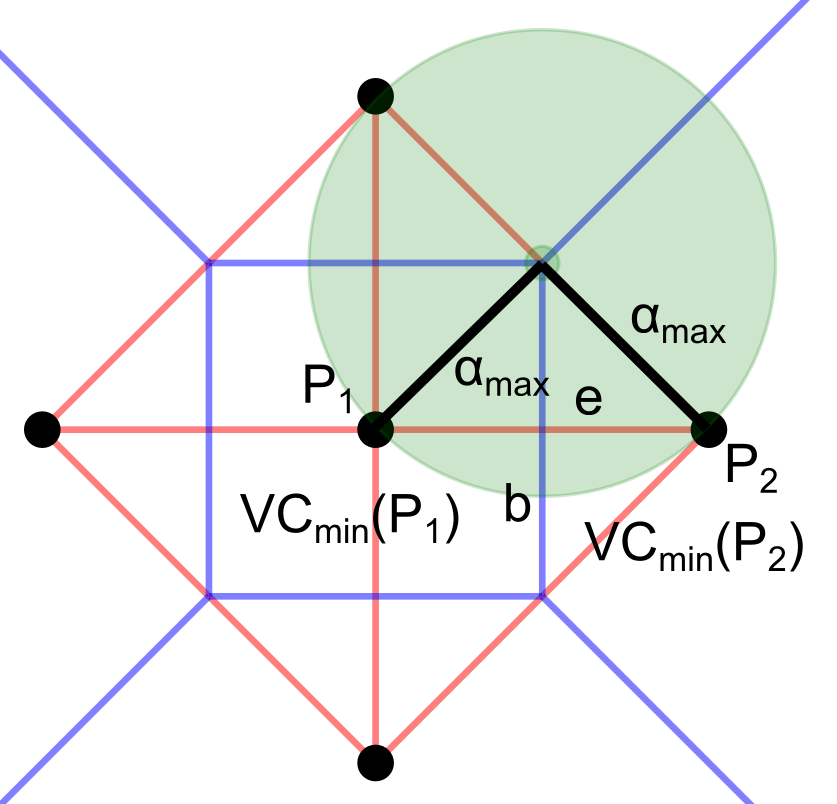
\includegraphics[scale=0.7]{../bilder/alphaNeighbours_VDmin_alphaMax.png}}
	\caption{$\alpha_{\min}$ und $\alpha_{\max}$ für eine Kante $e$ aus $DG_{\min}$, deren Knoten nicht auf dem Rand der konvexen Hülle benachbart sind}
	\label{fig:alphaNeighbours_VDmin_alphaMinMax}	
\end{figure}

Abbildung~\ref{fig:alphaNeighbours_VDmin_alphaMinMax} zeigt Beispiele für die in Lemma \ref{lemma:alphaNeighbours_VDmin_alphaMinMax} geschilderte Situation.

\begin{proof}[Beweis zu Lemma \ref{lemma:alphaNeighbours_VDmin_alphaMinMax}]
Sei das Minimum-Voronoi-Diagramm von $S$ gegeben. Die Voronoi-Kante $b$ zwischen den Voronoi-Zellen mit den Zentren $P_1,P_2 \in S$ ist der einzige Ort für Mittelpunkte von positiven $\alpha$-Kreisscheiben, auf deren Rand $P_1$ und $P_2$ direkt benachbart sind. Der Radius einer solchen $\alpha$-Kreisscheibe muss mindestens gleich dem kleinsten Abstand von $P_1$ und $P_2$ zu $b$ sein. Der Radius kann höchstens gleich dem größten Abstand von $P_1$ und $P_2$ zu $b$ sein.
\end{proof}

\begin{lemma}\label{lemma:alphaNeighbours_VDmin_Konvex}
Sei $e=(P_1,P_2)$ eine Kante des Minimum-Delaunay-Graphen von $S$. Seien $P_1,P_2 \in S$ direkt auf dem Rand der konvexen Hülle von $S$ benachbart. Sei $b$ die Voronoi-Kante zwischen den Voronoi-Zellen mit den Zentren $P_1$ und $P_2$. Dann gilt $Sp^+(e) = [\alpha_{\min}, \infty)$. $\alpha_{\min}$ ist der minimale Abstand von $P_1$ und $P_2$ zu $b$.
\end{lemma}

\begin{figure}[htbp]
	\centering
	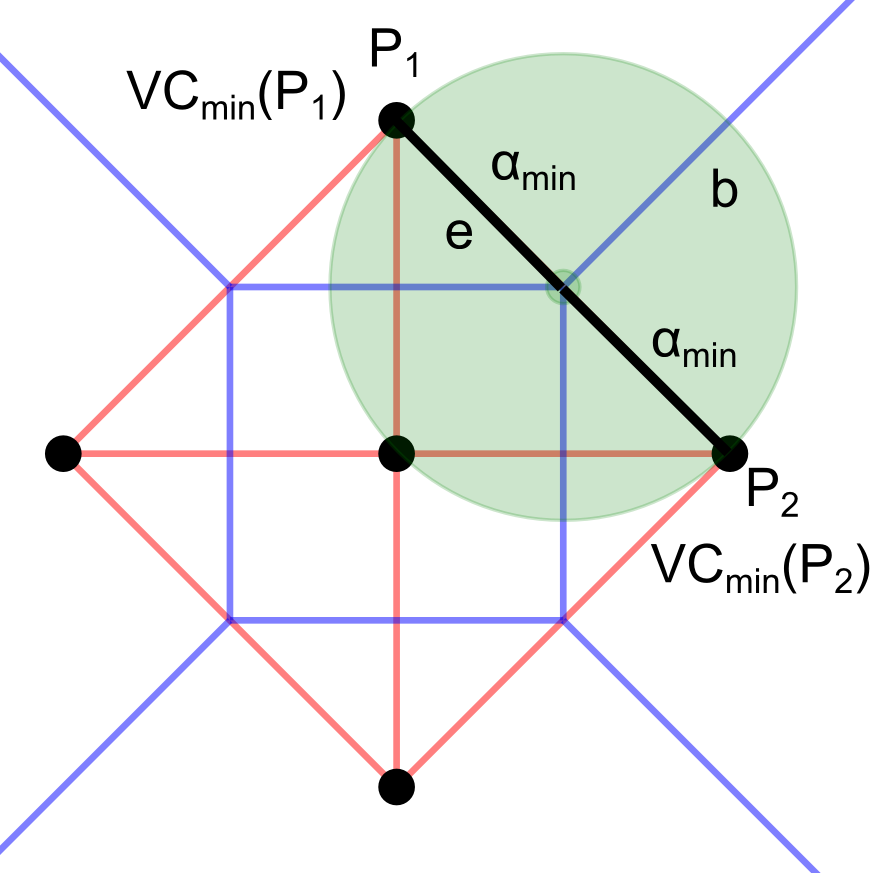
\includegraphics[scale=0.7]{../bilder/alphaNeighbours_VDmin_Konvex.png}
	\caption{$\alpha_{\min}$ für eine Kante $e$ aus $DG_{\min}$, deren Knoten direkt auf dem Rand der konvexen Hülle benachbart sind}
	\label{fig:alphaNeighbours_VDmin_Konvex}
\end{figure}

Abbildung~\ref{fig:alphaNeighbours_VDmin_Konvex} zeigt Beispiele für die in Lemma \ref{lemma:alphaNeighbours_VDmin_Konvex} geschilderte Situation.

\begin{proof}[Beweis zu Lemma \ref{lemma:alphaNeighbours_VDmin_Konvex}]
Sei das Minimum-Voronoi-Diagramm von $S$ gegeben. Die Voronoi-Kante $b$ zwischen den Voronoi-Zellen mit den Zentren $P_1,P_2 \in S$ ist der einzige Ort für Mittelpunkte von positiven $\alpha$-Kreisscheiben, auf deren Rand $P_1$ und $P_2$ direkt benachbart sind. Der Radius einer solchen $\alpha$-Kreisscheibe muss mindestens gleich dem kleinsten Abstand von $P_1$ und $P_2$ zu $b$ sein. Der Radius ist nicht nach oben beschränkt, da $b$ in dem in Lemma \ref{lemma:alphaNeighbours_VDmin_Konvex} geschilderten Fall ein Strahl ist.
\end{proof}

\begin{lemma}\label{lemma:alphaNeighbours_VDmax_alphaMinMax}
Sei $e=(P_1,P_2)$ eine Kante des Maximum-Delaunay-Graphen von $S$. Seien $P_1,P_2 \in S$ nicht direkt auf dem Rand der konvexen Hülle von $S$ benachbart. Sei $b$ die Voronoi-Kante zwischen den Voronoi-Zellen mit den Zentren $P_1$ und $P_2$. Dann gilt $Sp^-(e) = [\alpha_{\min}, \alpha_{\max}]$. $\alpha_{\min}$ ist die Negation des maximalen und $\alpha_{\max}$ die Negation des minimalen Abstands von $P_1$ und $P_2$ zu $b$.
\end{lemma}

\begin{figure}[htbp]
	\centering
	\subfloat[$\alpha_{\min}$ für Kante $e$ aus $DG_{\max}$ deren Knoten nicht auf dem Rand der konvexen Hülle benachbart sind\label{fig:alphaNeighbours_VDmax_alphaMin}]
		{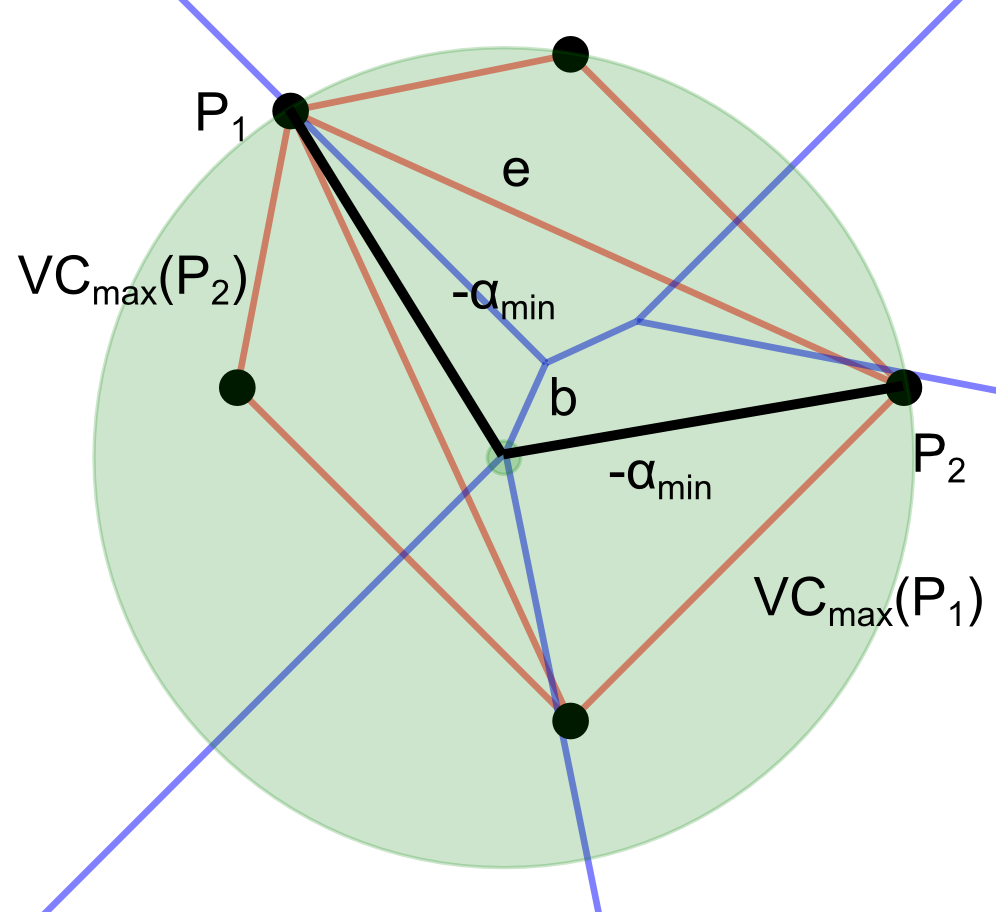
\includegraphics[scale=0.7]{../bilder/alphaNeighbours_VDmax_alphaMin.png}}
	\hspace{2cm}
	\subfloat[$\alpha_{\max}$ für Kante $e$ aus $DG_{\max}$ deren Knoten nicht auf dem Rand der konvexen Hülle benachbart sind\label{fig:alphaNeighbours_VDmax_alphaMax}]
		{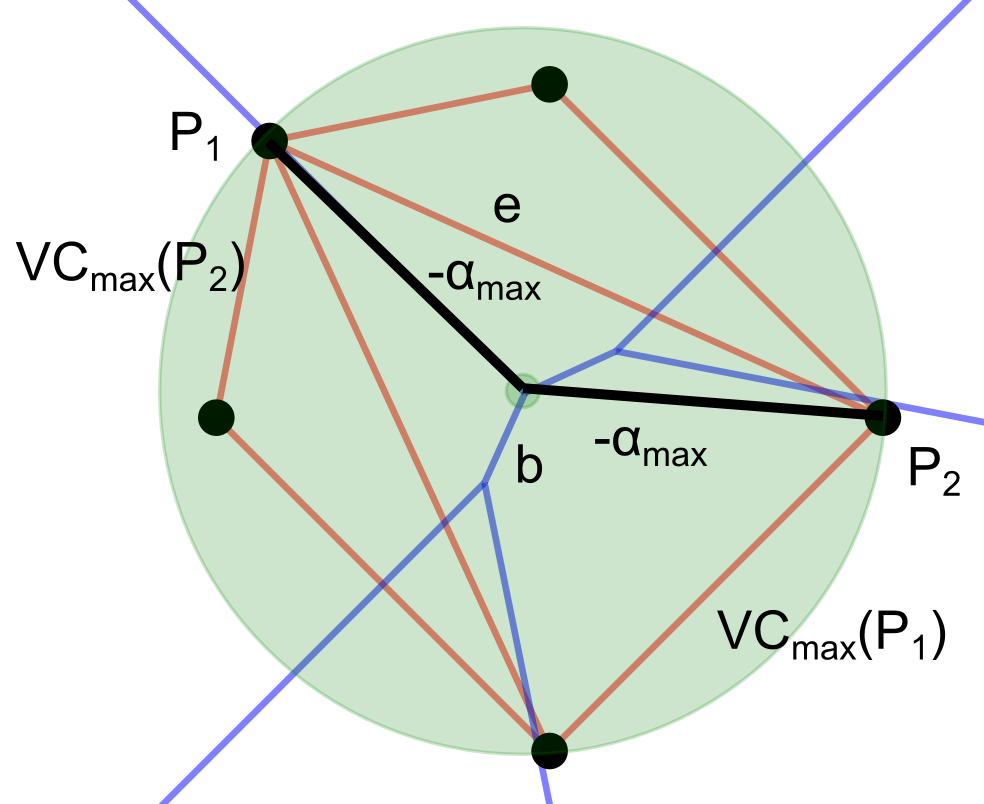
\includegraphics[scale=0.7]{../bilder/alphaNeighbours_VDmax_alphaMax.png}}
	\caption{$\alpha_{\min}$ und $\alpha_{\max}$ für eine Kante $e$ aus $DG_{\max}$ deren Knoten nicht auf dem Rand der konvexen Hülle benachbart sind}
	\label{fig:alphaNeighbours_VDmax_alphaMinMax}	
\end{figure}

Abbildung~\ref{fig:alphaNeighbours_VDmax_alphaMinMax} zeigt Beispiele für die in Lemma \ref{lemma:alphaNeighbours_VDmax_alphaMinMax} geschilderte Situation.

\begin{proof}[Beweis zu Lemma \ref{lemma:alphaNeighbours_VDmax_alphaMinMax}]
Sei das Maximum-Voronoi-Diagramm von $S$ gegeben. Die Voronoi-Kante $b$ zwischen den Voronoi-Zellen mit den Zentren $P_1,P_2 \in S$ ist der einzige Ort für Mittelpunkte von negativen $\alpha$-Kreisscheiben, auf deren Rand $P_1$ und $P_2$ direkt benachbart sind. Der Radius einer solchen $\alpha$-Kreisscheibe muss mindestens gleich dem kleinsten Abstand von $P_1$ und $P_2$ zu $b$ sein. Der Radius kann höchstens gleich dem größten Abstand von $P_1$ und $P_2$ zu $b$ sein.
\end{proof}

\begin{lemma}\label{lemma:alphaNeighbours_VDmax_Konvex}
Sei $e=(P_1,P_2)$ eine Kante des Maximum-Delaunay-Graphen von $S$. Seien $P_1,P_2 \in S$ direkt auf dem Rand der konvexen Hülle von $S$ benachbart. Sei $b$ die Voronoi-Kante zwischen den Voronoi-Zellen mit den Zentren $P_1$ und $P_2$. Dann gilt $Sp^-(e) = (-\infty, \alpha_{\max}]$. $\alpha_{\max}$ ist die Negation des minimale Abstands von $P_1$ und $P_2$ zu $b$.
\end{lemma}

\begin{figure}[htbp]
	\centering
	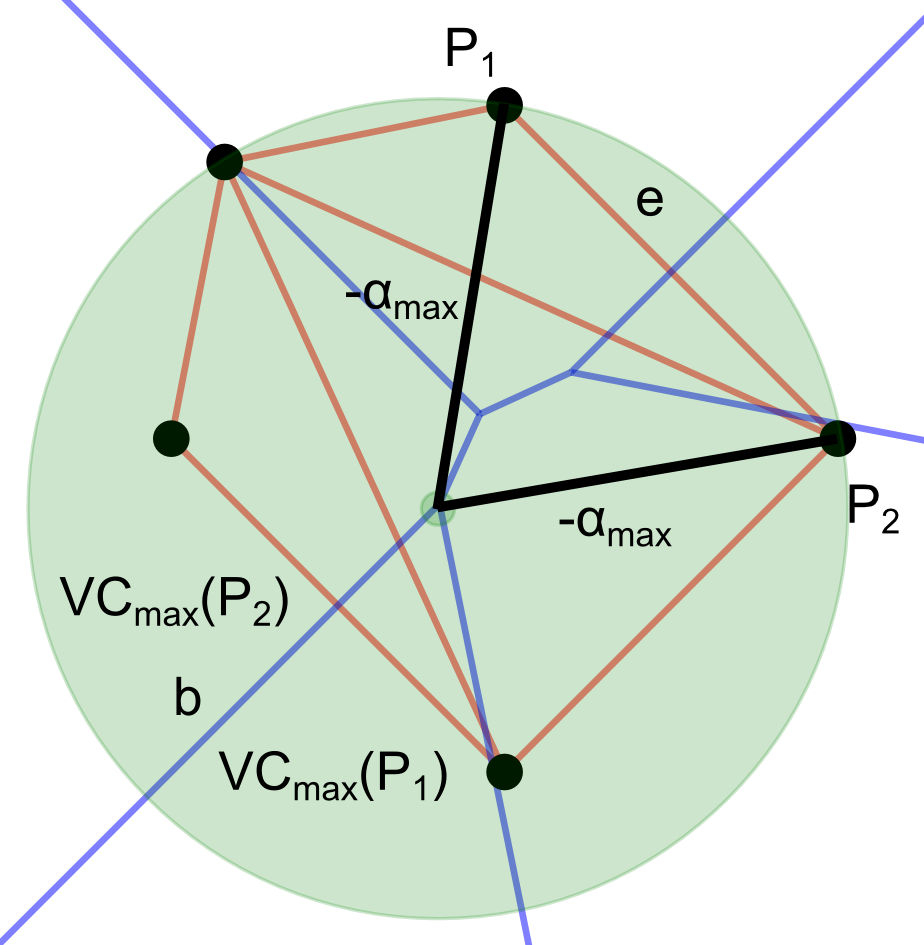
\includegraphics[scale=0.7]{../bilder/alphaNeighbours_VDmax_Konvex.png}
	\caption{$\alpha_{\max}$ für eine Kante $e$ aus $DG_{\max}$ deren Knoten direkt auf dem Rand der konvexen Hülle benachbart sind}
	\label{fig:alphaNeighbours_VDmax_Konvex}
\end{figure}

Abbildung~\ref{fig:alphaNeighbours_VDmax_Konvex} zeigt Beispiele für die in Lemma \ref{lemma:alphaNeighbours_VDmax_Konvex} geschilderte Situation.

\begin{proof}[Beweis zu Lemma \ref{lemma:alphaNeighbours_VDmax_Konvex}]
Sei das Maximum-Voronoi-Diagramm von $S$ gegeben. Die Voronoi-Kante $b$ zwischen den Voronoi-Zellen mit den Zentren $P_1,P_2 \in S$ ist der einzige Ort für Mittelpunkte von negativen $\alpha$-Kreisscheiben, auf deren Rand $P_1$ und $P_2$ direkt benachbart sind. Der Radius einer solchen $\alpha$-Kreisscheibe muss mindestens gleich dem kleinsten Abstand von $P_1$ und $P_2$ zu $b$ sein. Der Radius ist nicht nach oben beschränkt, da $b$ in dem in Lemma \ref{lemma:alphaNeighbours_VDmax_Konvex} geschilderten Fall ein Strahl ist.
\end{proof}

In Lemma \ref{lemma:alphaExtreme_VDmin_alphaMax} - \ref{lemma:alphaNeighbours_VDmax_Konvex} wurde gezeigt, dass die Shape-Spektren von Knoten und Kanten des Delaunay-Graphen Intervalle sind.

Eine Shape-Schwelle ist eine Schwelle, bei deren Überschreiten sich die $\alpha$-Shape ändert. Mit den Shape-Spektren können die Shape-Schwellen einer Punktmenge wie folgt definiert werden.

\begin{defin}
Die Menge der \emph{Shape-Schwellen einer Punktmenge $S$, $Bd(S)$}, ist die Menge der endlichen Grenzen ungleich Null der positiven und negativen Shape-Spektren aller Knoten und Kanten des Minimum- und Maximum-Delaunay-Graphen von $S$.
\end{defin}

% !TEX encoding = UTF-8 Unicode

\chapter{Konstruktion der \boldmath{$\alpha$}-Shape}

Im vorherigen Kapitel wurde gezeigt, dass die $\alpha$-Shape ein Subgraph des Delaunay-Graphen ist und es wurden die Shape-Spektren sowie die Shape-Schwellen definiert.

Hier wird nun ein Algorithmus gezeigt, welcher aus Minimum- und Maximum-Voronoi-Diagrammen einer Punktmenge $S$ die Shape-Spektren der Delaunay-Graphen von $S$ sowie die Shape-Schwellen von $S$ bestimmt. Anschließend wird ein Algorithmus gezeigt, welcher, mit $\alpha$ und den Shape-Spektren der Delaunay-Graphen von $S$ als Eingabe, die $\alpha$-Shape von $S$ bestimmt. Es werden weitere Algorithmen gezeigt, mit welchen, unter Ausnutzung des Shape-Spektrums, verschiedene interessante geometrische Eigenschaften von $S$ bestimmt werden können.

Zuerst wird kurz auf Algorithmen zur Erstellung von Voronoi-Diagrammen und auf die doppelt verkettete Kantenliste eingegangen. Dies ist der abstrakte Datentyp, in welchem die Voronoi-Diagramme für die Bestimmung von Shape-Spektren abgespeichert werden.

\section{Algorithmen zur Erstellung von Voronoi-Diagrammen}

Da die Erstellung von Voronoi-Diagrammen nicht das zentrale Thema dieser Arbeit ist, wird auf die implementierten Algorithmen und Datenstrukturen nur kurz eingegangen.

\subsection*{Fortunes Algorithmus}

In \autocite{deBerg2010} wird Fortunes Algorithmus zur Bestimmung eines \- Minimum-Voronoi-Diagramms beschrieben. Dabei handelt es sich um einen \- Plane-Sweep-Algo\-rithmus. Für die folgende Betrachtung wird die Sweep-Line von oben nach unten über die Ebene bewegt.

Die Bereiche oberhalb der Sweep-Line, welche sich im Voronoi-Diagramm nicht mehr ändern, werden durch sich schneidende Parabelbögen, der sogenannten Küstenlinie, bestimmt. Die Küstenlinie wird in einem AVL-Baum, wie er in \autocite{Gueting2004} beschrieben wird, gespeichert. Die innere Knoten des Baums sind die Schnittpunkte und seine Blätter sind die Parabelbögen. Der Verlauf der Schnittpunkte der Parabelbögen bestimmt den Verlauf der Kanten im Voronoi-Diagramm. Verschwindet ein Parabelbogen, so ist an dieser Stelle ein Knoten.

\begin{figure}[htbp]
	\centering
	\subfloat[Küstenlinie\label{fig:beachline}]
		{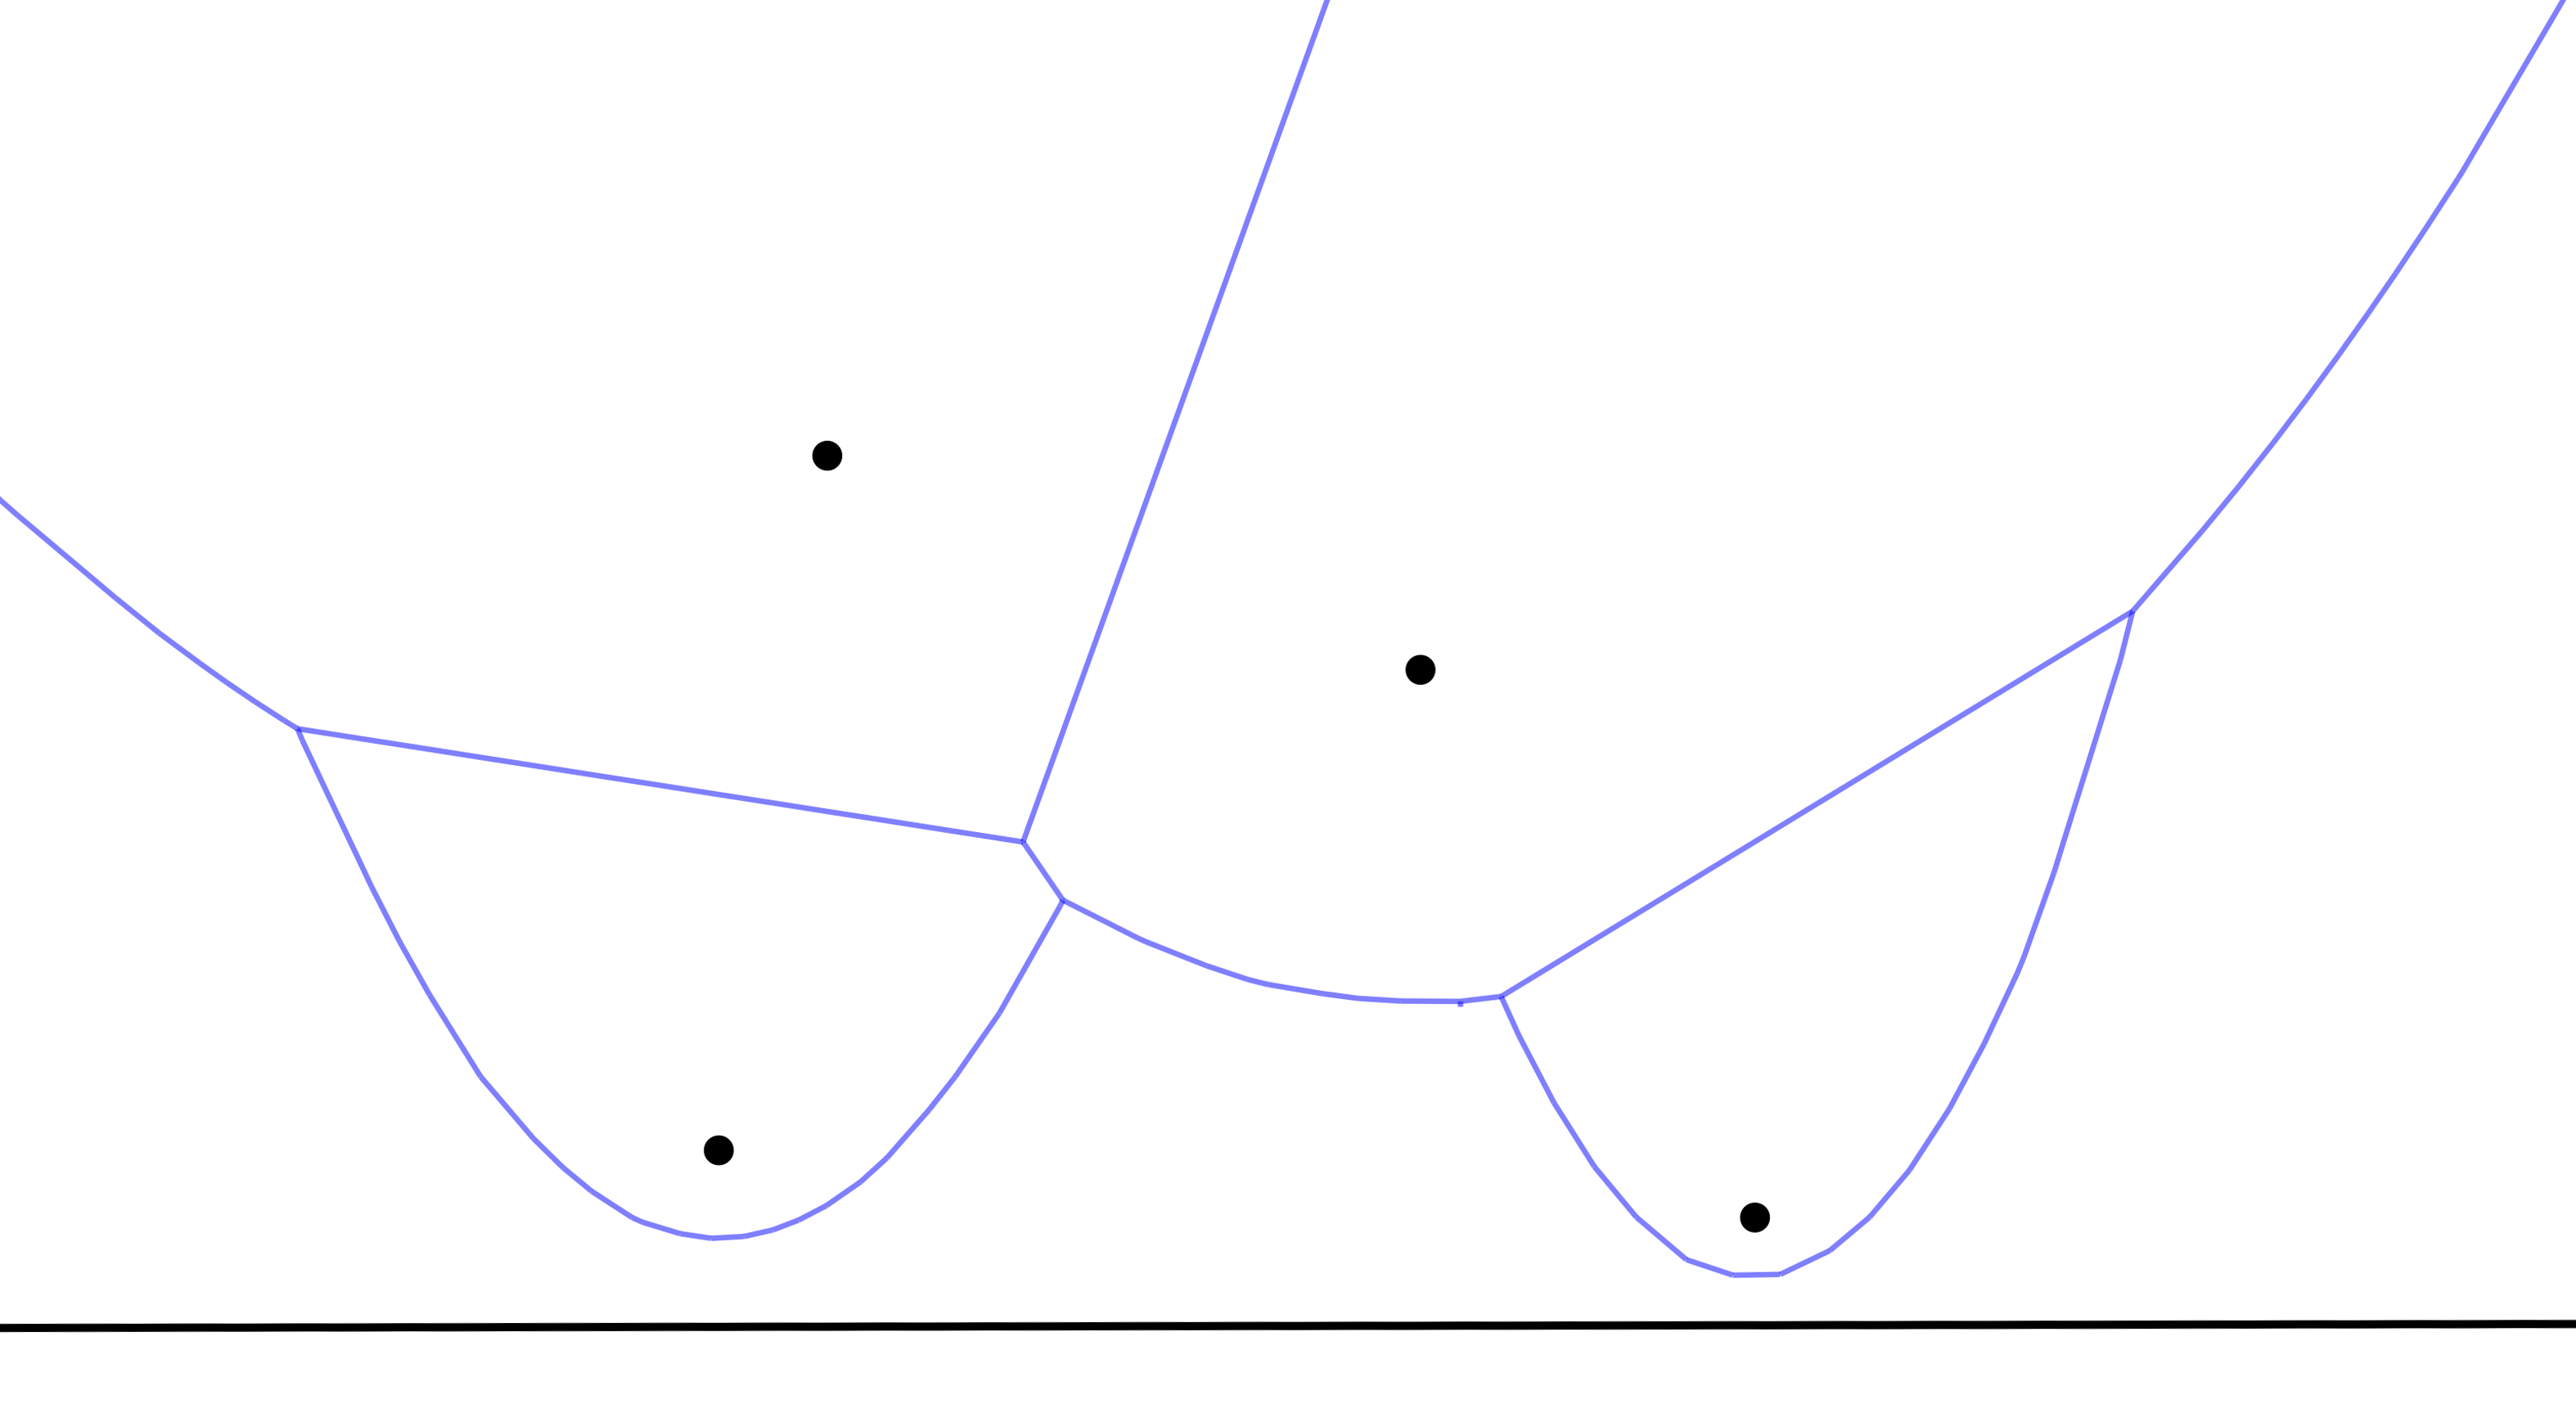
\includegraphics[scale=0.5]{../bilder/beachline.png}}
	\hspace{2cm}
	\subfloat[AVL-Baum\label{fig:beachline_tree}]
		{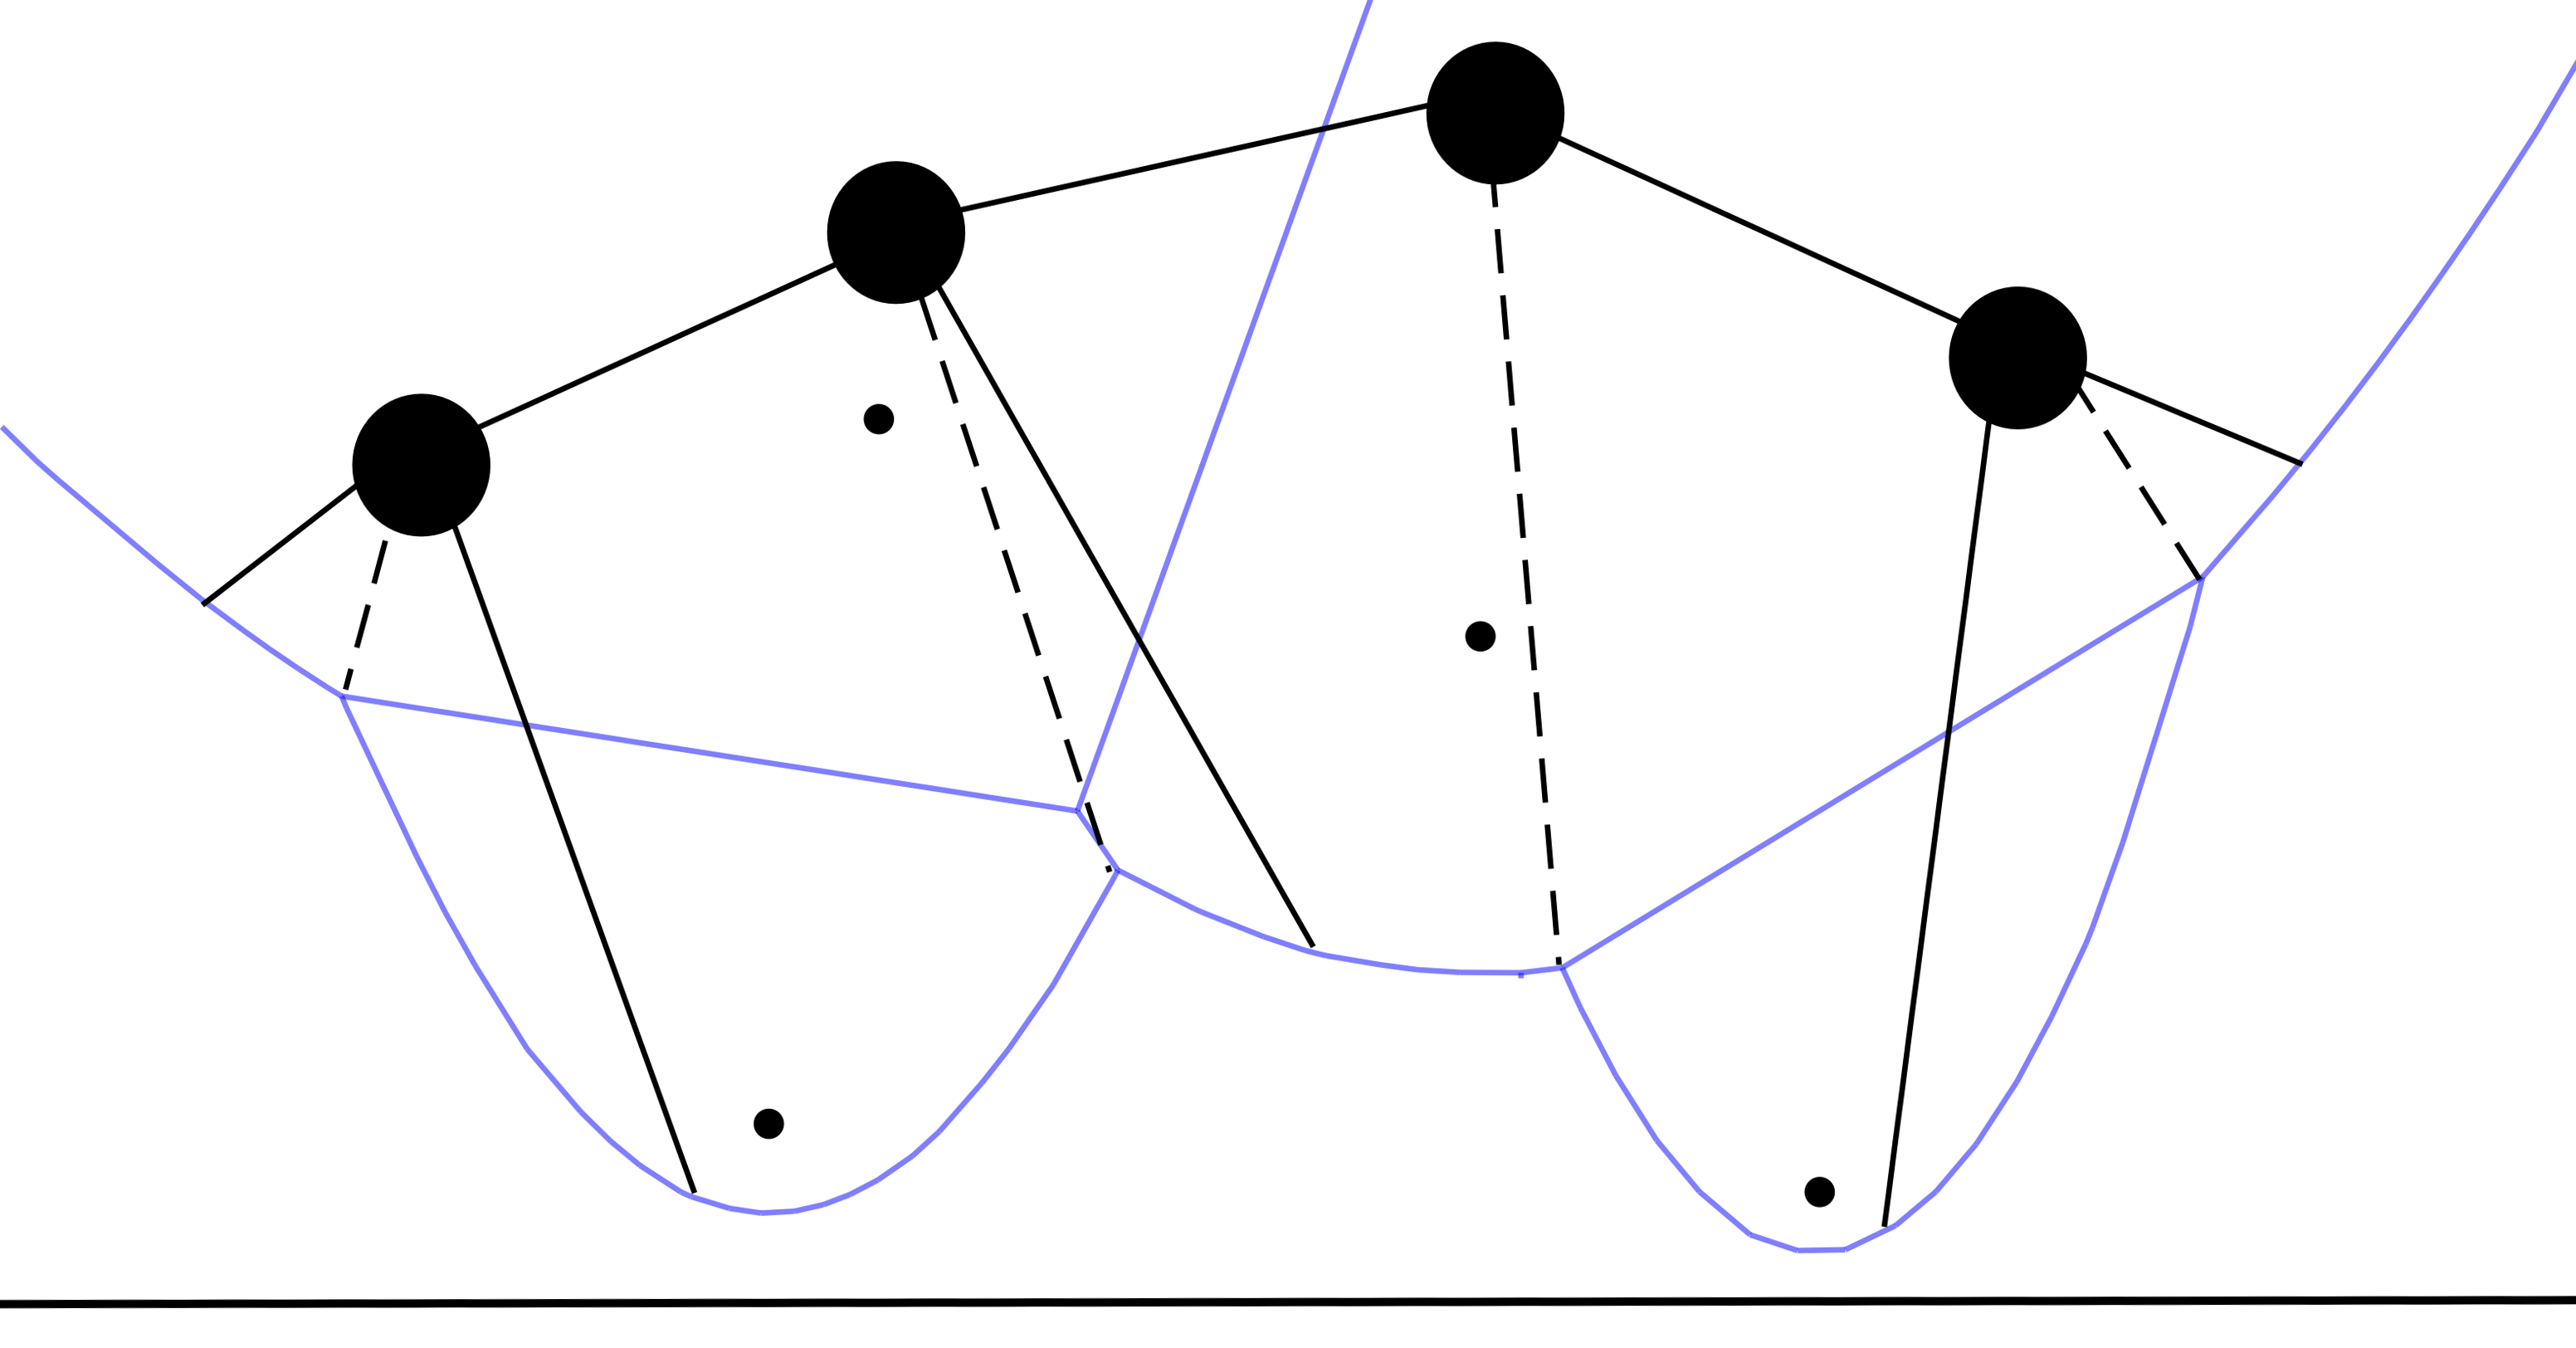
\includegraphics[scale=0.5]{../bilder/beachline_tree.png}}
	\caption{Küstenlinie und AVL-Baum für Fortunes Algorithmus}
	\label{fig:fortune}	
\end{figure}

In Abbildung~\ref{fig:fortune} wird eine Punktmenge, eine Sweep-Line, eine Küstenlinie und der AVL-Baum zur Speicherung der Küstenlinie dargestellt. Die gestrichelten Linien stellen die Zuordnung von inneren Knoten zu Schnittpunkten dar und sind keine Kanten des Baums.

Trifft die Sweep-Line auf einen Punkt aus $S$, so muss ein neuer Parabelbogen in die Küstenlinie eingefügt werden. Liegen die Punkte dreier benachbarter Parabelbögen auf einem Kreis und trifft die Sweep-Line den tiefsten Punkt dieses Kreises, so muss ein Parabelbogen sowie ein Schnittpunkt aus der Küstenlinie entfernt werden.

Einfügen und entfernen eines Knoten hat für einen AVL-Baum mit $n$ Knoten eine Zeitkomplexität von $O(\log{n})$. Für eine Punktmenge mit $n$ Punkten ergibt sich damit eine Gesamtzeitkomplexität für die Bestimmung des Minimum-Vornoi-Diagramms von $O(n \log{n})$.

\subsection*{Algorithmus von Skyum}

Skyum beschreibt in \autocite{skyum1991} einen Algorithmus, welcher aus den Punkten auf der konvexen Hülle einer Punktmenge deren Maximum-Voronoi-Diagramm bestimmt. Durch je zwei aufeinanderfolgende Punkte auf der konvexen Hülle werden die Knoten "`im Unendlichen"' bestimmt. Um die restlichen Knoten zu bestimmen, werden aus je drei aufeinanderfolgenden Punkten, $P_1,P_2,P_3$, auf der konvexen Hülle Dreiecke gebildet. Diese werden nach Umkreisradius und Winkel bei $P_2$ sortiert. Zu dem Dreieck mit maximalen Umkreisradius bzw. Winkel wird der Umkreismittelpunkt bestimmt. Der Umkreismittelpunkt ist ein Knoten. Anschließend wird $P_2$ aus der Eingabepunktmenge entfernt, wodurch sich ggf. neue Dreiecke ergeben. Es werden alle Dreiecke, an denen $P_2$ beteiligt ist, aus der Sequenz der Dreiecke entfernt. Die neuen Dreiecke werden in die sortierte Sequenz der Dreiecke eingefügt. Das Maximum-Voronoi-Diagramm ist fertig, sobald kein Dreieck mehr in der Sequenz ist.

Der Algorithmus hat für eine Punktmenge mit $n$ Punkten eine Laufzeitkomplexität von $O(n \log{n})$. Die Punkte auf der konvexen Hülle werden durch das Konturpolygonverfahren, welches in \autocite{ProPra2012} beschrieben ist, bestimmt. Dieses Verfahren hat ebenfalls eine Laufzeitkomplexität von $O(n \log{n})$ für eine Punktmenge mit $n$ Punkten.

\subsection*{Die Doppelt Verkettete Kantenliste}

Die \emph{doppelt verkettete Kantenliste}, kurz \emph{DVK}, ist ein abstrakter Datentyp zur Repräsentation von Graphen. Sie wird in \autocite{deBerg2010} beschrieben. Die DVK enthält je eine Menge für Knoten, Flächen und Halb-Kanten. Daher kann leicht über die entsprechenden Elemente iteriert werden.

Ein \emph{Knoten} enthält seine Koordinaten und eine Referenz auf eine beliebige Halb-Kante, welche den Knoten als Ursprung hat.

Eine \emph{Fläche} enthält eine Referenz auf ihre äußere Komponente und auf jede innere Komponente. Die äußere Komponente ist eine Halb-Kante, welche zur äußeren Begrenzung beiträgt und eine innere Komponente ist eine Halb-Kante, welche zur Begrenzung eines Loches in der Fläche beiträgt. Für die Speicherung von Voronoi-Zellen als Flächen, enthält die Fläche zusätzlich noch die Koordinaten des Zentrums der Voronoi-Zelle.

Eine \emph{Halb-Kante} hat eine Referenz auf ihren Ursprungsknoten, auf ihre Vorgänger-Halb-Kante, auf ihre Nachfolger-Halb-Kante, auf eine Fläche, zu deren Kantenmenge sie gehört, und auf ihre Zwillings-Halb-Kante. Die Kombination aus Halb-Kante und Zwilling wird im Folgenden einfach als \emph{Kante} bezeichnet.


\begin{figure}[htbp]
	\centering
	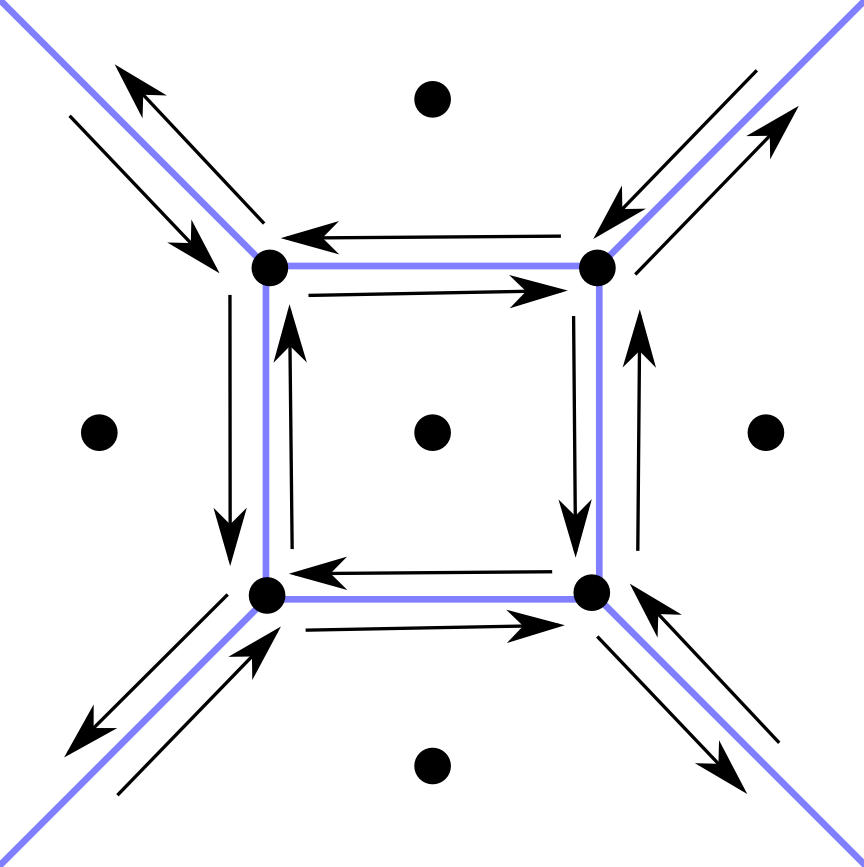
\includegraphics[scale=1.0]{../bilder/voronoi_min_dcel.png}
	\caption{DVK eines Minimum-Voronoi-Diagramms}
	\label{fig:voronoi_min_dcel}
\end{figure}

In Abbildung~\ref{fig:voronoi_min_dcel} ist die DVK eines Minimum-Voronoi-Diagramms dargestellt. Die Halb-Kanten liegen in den von ihnen begrenzten Flächen und sind im Uhrzeigersinn verkettet. Der Zwilling jeder Halb-Kante liegt in einer benachbarten Fläche bzw. Voronoi-Zelle. Knoten des Diagramms und die Zentren der Flächen sind als schwarze Punkte dargestellt.

\section{Ein Algorithmus zur Bestimmung der Shape-Spektren}

Vor der Beschreibung des Algorithmus werden wichtige Teilschritte erklärt und es wird auf den Umgang mit unendlich langen Kanten im Voronoi-Diagramm eingegangen.

\subsection*{Bestimmung eines Knotens des Delaunay-Graphen aus der DVK eines Voronoi-Diagramms}

Ein Knoten des Delaunay-Graphen und die Grenzen seines Shape-Spektrums können aus einer Flächen $f(P)$ der DVK eines Voronoi-Diagramms bestimmt werden. Jedes Zentrum $P$ einer Fläche ist auch ein Knoten des Delaunay-Graphen und umgekehrt. Um das Shape-Spektrum des Knotens zu bestimmen muss der Abstand von $P$ zu allen Vorgänger- und Nachfolger-Kanten der äußeren Komponente der Fläche bestimmt werden. Sei nun $d_{\min}(f(P))$ der minimale und $d_{\max}(f(P))$ der maximale dieser Abstände.

\subsection*{Bestimmung einer Kante des Delaunay-Graphen aus der DVK eines Voronoi-Diagramms}

Eine Kante des Delaunay-Graphen und die Grenzen seines Shape-Spektrums können aus einer Kante $b$ der DVK eines Voronoi-Diagramms bestimmt werden. Jeder Kante $b$ des Voronoi-Diagramms ist eine eindeutige duale Kante $e$ des Delaunay-Graphen zugeordnet und umgekehrt. Anfangs- und Endpunkt von $e$ sind die Zentren derjenigen Flächen, welche durch $b$ getrennt werden. Um das Shape-Spektrum der Kante $e$ zu bestimmen muss der minimale und der maximale Abstand eines Endpunkts von $e$ zu $b$ bestimmt werden. Sei nun $d_{\min}(e,b)$ der minimale und $d_{\max}(e,b)$ der maximale Abstand.

\subsection*{Eine untere Schranke für unendliche Abstände im Voronoi-Diagramm}

In einem Voronoi-Diagramm können Kanten vorkommen, welche Strahlen oder Geraden sind. Diese Kanten werden für die praktische Berechnung durch Strecken angenähert. Die Länge dieser Strecken muss größer sein als der maximal vorkommende Abstand eines Zentrums einer abgeschlossenen Voronoi-Zelle zu ihrem Rand. Dieser Wert wird durch die Konstante \emph{BIGVAL} repräsentiert. Alle Abstände im Voronoi-Diagramm, welche größer sind als dieser Wert, gelten als unendlich. Der Wert von \emph{BIGVAL} ist abhängig von den Koordinaten der Eingabepunktmenge und muss an diese angepasst werden. Für praktische Anwendungen wurde das zehnfache des maximal zu erwartenden Abstands zweier Punkte verwendet. Wird zur Eingabe einer Punktmenge eine rechteckige Zeichenfläche verwendet wird, so ist der maximale Abstand zweier Punkte gleich der Diagonalen dieser Zeichenfläche.

\subsection*{Der Algorithmus}

Die Eingabe des Algorithmus zur Bestimmung der Shape-Spektren ist eine Punktmenge $S$. Seine Ausgabe ist die Menge der positiven Shape-Spektren der Knoten und Kanten des Minimum-Delaunay-Graphen von $S$, $PV(S)$ und $PE(S)$, die Menge der negativen Shape-Spektren der Knoten und Kanten des Maximum-Delaunay-Graphen von $S$, $NV(S)$ und $NE(S)$, sowie die positiven und negativen Shape-Schwellen der Punktmenge, $Bd^+(S)$ und $Bd^-(S)$. Aus Gründen der Übersichtlichkeit ist der Algorithmus in einen Algorithmus zur Bestimmung der positiven Shape-Spektren (Algorithmus~\ref{alg:posSpec}) und einen Algorithmus zur Bestimmung der negativen Shape-Spektren (Algorithmus~\ref{alg:negSpec}) aufgeteilt worden.

\begin{algorithm}\caption{Bestimmung der positiven Shape-Spektren}\label{alg:posSpec}
\begin{algorithmic}[0]
\Function{PositiveShapeSpektren}{$S$}
	\State $PV(S) \gets \oslash$
	\State $PE(S) \gets \oslash$
	\State $Bd^+(S) \gets \oslash$
	\State Bestimme DVK von $VD_{\min}(S)$
	\ForAll{$f(P) \in VD_{\min}(S)$}
		\If{$d_{\max}(f(P)) < \text{ BIGVAL}$}
			\State $Sp^+(P) \gets (0, d_{\max}(f(P))]$
			\State $Bd^+(S) \gets Bd^+(S) \cup \lbrace d_{\max}(f(P)) \rbrace$
		\Else
			\State $Sp^+(P) \gets (0, \infty)$
		\EndIf
		\State $PV(S) \gets PV(S) \cup \lbrace Sp^+(P) \rbrace$
	\EndFor
	\ForAll{$b \in VD_{\min}(S)$}
		\State Bestimme duale Delaunay-Kante $e$ zu $b$
		\State $Bd^+(S) \gets Bd^+(S) \cup \lbrace d_{\min}(e,b) \rbrace$
		\If{$d_{\max}(e,b) < \text{ BIGVAL}$}
			\State $Sp^+(e) \gets [d_{\min}(e,b),d_{\max}(e,b)]$
			\State $Bd^+(S) \gets Bd^+(S) \cup \lbrace d_{\max}(e,b) \rbrace$
		\Else
			\State $Sp^+(e) \gets [d_{\min}(e,b),\infty)$
		\EndIf
		\State $PE(S) \gets PE(S) \cup \lbrace Sp^+(e) \rbrace$
	\EndFor
	\State \textbf{return} $(PV(S),PE(S),Bd^+(S))$
\EndFunction
\end{algorithmic}
\end{algorithm}

\begin{algorithm}\caption{Bestimmung der negative Shape-Spektren}\label{alg:negSpec}
\begin{algorithmic}[0]
\Function{NegativeShapeSpektren}{$S$}
	\State $NV(S) \gets \oslash$
	\State $NE(S) \gets \oslash$
	\State $Bd^-(S) \gets \oslash$
	\State Bestimme DVK von $VD_{\max}(S)$
	\ForAll{$f(P) \in VD_{\max}(S)$}
		\State $Sp^-(P) \gets (-\infty,-d_{\min}(f(P))]$
		\State $Bd^-(S) \gets Bd^-(S) \cup \lbrace -d_{\min}(f(P)) \rbrace$
		\State $NV(S) \gets NV(S) \cup \lbrace Sp^-(P) \rbrace$
	\EndFor
	\ForAll{$b \in VD_{\max}(S)$}
		\State Bestimme duale Delaunay-Kante $e$ zu $b$
		\State $Bd^-(S) \gets Bd^-(S) \cup \lbrace d_{\min}(e,b) \rbrace$
		\If{$d_{\max} < \text{ BIGVAL}$}
			\State $Sp^-(e) \gets [-d_{\max}(e,b),-d_{\min}(e,b)]$
			\State $Bd^-(S) \gets Bd^-(S) \cup \lbrace -d_{\max} \rbrace$
		\Else
			\State $Sp^-(e) \gets (-\infty,-d_{\min}(e,b)]$
		\EndIf
		\State $NE(S) \gets NE(S) \cup \lbrace Sp^-(e) \rbrace$
	\EndFor
	\State \textbf{return} $(NV(S),NE(S),Bd^-(S))$
\EndFunction
\end{algorithmic}
\end{algorithm}

\begin{lemma}\label{lemma:shape_compl}
Die Zeitkomplexität für die Bestimmung der Shape-Spektren bezüglich der Größe $n$ der Punktmenge $S$ ist $O(n \log{n})$.
\end{lemma}

\begin{proof}[Beweis zu Lemma \ref{lemma:shape_compl}]
Die Algorithmen zur Berechnung der Voronoi-Diagramme von $S$ haben eine Zeitkomplexität von $O(n \log{n})$. Die Anzahl der Zellen und Kanten im Voronoi-Diagramm ist linear zu $n$. Es wird ein Shape-Spektrum pro Kante und ein Shape-Spektrum pro Zentrum je mit konstanter Zeitkomplexität berechnet. Damit ist die Zeitkomplexität der Berechnung aller Kanten- und Knoten-Shape-Spektren linear zu $n$.
\end{proof}

\section[Ein Algorithmus zur Konstruktion der $\alpha$-Shape]{Ein Algorithmus zur Konstruktion der \boldmath{$\alpha$}-Shape}

Die Eingabe des Algorithmus zur Bestimmung der $\alpha$-Shape (Algorithmus~\ref{alg:shape}) ist der Parameter $\alpha$, die Menge der positiven Shape-Spektren der Knoten und Kanten des Minimum-Delaunay-Graphen von $S$, $PV(S)$ und $PE(S)$, sowie die Menge der negativen Shape-Spektren der Knoten und Kanten des Maximum-Delaunay-Graphen von $S$, $NV(S)$ und $NE(S)$. Seine Ausgabe ist die Menge der Knoten der $\alpha$-Shape von $S$, $AV(S,\alpha)$, und die Menge der Kanten der $\alpha$-Shape von $S$, $AE(S,\alpha)$.

\begin{algorithm}\caption{Bestimmung der $\alpha$-Shape}\label{alg:shape}
\begin{algorithmic}[0]
\Function{AlphaShape}{$\alpha,PV(S),PE(S),NV(S),NE(S)$}
	\State $AV(S,\alpha) \gets \oslash$
	\State $AE(S,\alpha) \gets \oslash$
	\If{$\alpha > 0$}
		\ForAll{$Sp^+(P) \in PV(S)$}
			\If{$\alpha \in Sp^+(P)$}
				$AV(S,\alpha) \gets AV(S,\alpha) \cup \lbrace P \rbrace$
			\EndIf
		\EndFor
		\ForAll{$Sp^+(e) \in PE(S)$}
			\If{$\alpha \in Sp^+(e)$}
				$AE(S,\alpha) \gets AE(S,\alpha) \cup \lbrace e \rbrace$
			\EndIf
		\EndFor
	\ElsIf{$\alpha < 0$}
		\ForAll{$Sp^-(P) \in NV(S)$}
			\If{$\alpha \in Sp^-(P)$}
				$AV(S,\alpha) \gets AV(S,\alpha) \cup \lbrace P \rbrace$
			\EndIf
		\EndFor
		\ForAll{$Sp^-(e) \in PE(S)$}
			\If{$\alpha \in Sp^-(e)$}
				$AE(S,\alpha) \gets AE(S,\alpha) \cup \lbrace e \rbrace$
			\EndIf
		\EndFor
	\EndIf	
	\State \textbf{return} $(AV(S,\alpha),AE(S,\alpha))$
\EndFunction
\end{algorithmic}
\end{algorithm}

\begin{lemma}\label{lemma:alpha_compl}
Die Zeitkomplexität für die Bestimmung der $\alpha$-Shape aus Shape-Spektren bezüglich der Größe $n$ der Punktmenge $S$ ist linear.
\end{lemma}

\begin{proof}[Beweis zu Lemma \ref{lemma:alpha_compl}]
Die Mächtigkeit der Mengen der Shape-Spektren verhält sich linear zu $n$.
\end{proof}

\section{Shape-Spektrum-Algorithmen}

Mit Hilfe von Shape-Spektren lassen sich auch noch andere interessante Eigenschaften von Punktmengen bestimmen.

\subsection*{Das dichteste Paar}
Der Abstand des dichtesten Paares einer Punktmenge $S$ ist das doppelte des kleinsten Wertes in $Bd^+(S)$. Das dichteste Paar selbst lässt sich bestimmen, indem man in der Menge $PE(S)$ dasjenige $Sp^+(e)$ mit $e=(P_1,P_2)$ sucht, dessen untere Schranke gleich dem kleinsten positiven Wert ist. Das dichteste Paar ist dann $(P_1,P_2)$.

\subsection*{Der kleinste einschließende Kreis}
Der Radius $r$ des kleinsten einschließenden Kreises einer Punktmenge $S$ ist der kleinste Betrag in $Bd^-(S)$. Der Mittelpunkt des kleinsten einschließenden Kreises lässt sich folgendermaßen bestimmen: Man sucht in der Menge $NE(S)$ diejenigen $Sp^-(e)$, deren obere Schranke gleich der Negation von $r$ ist. Existiert nur ein solches $Sp^-(e)$, so ist der Mittelpunkt von $e$ auch der Mittelpunkt des kleinsten Kreises. Existieren mehrere solche $Sp^-(e)$, so bilden die Kanten $e$ ein Polygon, dessen Umkreis-Mittelpunkt der Mittelpunkt des kleinsten einschließenden Kreises ist.

\subsection*{Der Rand der konvexen Hülle}
Die konvexe Hülle lässt sich folgendermaßen bestimmen: Suche in der Menge $PE(S)$ diejenigen $Sp^+(e)$, deren obere Schranke gleich $\infty$ ist. Alternativ kann man auch in der Menge $NE(S)$ nach denjenigen $Sp^-(e)$ suchen, deren untere Schranke gleich $-\infty$ ist. Der Rand der konvexen Hülle ist gleich der Menge der Kanten $e$.

% !TEX encoding = UTF-8 Unicode

\chapter{Die \boldmath{$\alpha$}-Shapes-Applikation}

Die $\alpha$-Shapes-Applikation ist eine HTML5-Applikation, welche es ermöglicht \- Punktmengen zu erstellen und die $\alpha$-Shape für ein wählbares $\alpha$ darzustellen.

Darüber hinaus lassen sich noch andere Eigenschaften der Punktmenge visualisieren, welche im Zusammenhang mit der $\alpha$-Shape stehen.

Bei der Entwicklung dieser Applikation wurde Wert darauf gelegt, dass sie sowohl auf dem PC als auch auf mobilen Plattformen lauffähig und bedienbar ist. Da die meisten PCs und mobilen Geräte einen modernen Browser mit JavaScript Interpreter haben, wurde HTML5 als Technologie zur Implementierung ausgewählt.

Die Applikation ist mit einem Browser unter \autocite{alphaShapeHTML5} erreichbar. Zum Vergleich können unter \autocite{alpha_applet} auch mit einem Java Applet $\alpha$-Shapes erzeugt werden, welche näher an der Darstellung in \autocite{alpha1983} sind. Ein Nachteil bei der Verwendung eines Java Applets, im Vergleich zu HTML5, ist die Notwendigkeit eines Plugins. Dieses Plugin ist für viele Geräte nicht verfügbar.

\section{Funktionsbeschreibung}

Die Anwendung verfügt über verschiedene kombinierbare Anzeigemodi. In jedem Anzeigemodus wird eine andere Eigenschaft der Punktmenge visualisiert.

Ist kein Anzeigemodus ausgewählt, so werden nur die Punkte Punktmenge als kleine, schwarze Kreisscheiben dargestellt.

Es gibt folgende Anzeigemöglichkeiten:
\begin{itemize}
\item $\alpha$-Shape: Die $\alpha$-extremen Punkte werden transparent-rot umrandet. Die $\alpha$-Nachbarn werden durch fette, transparent-rote Linien verbunden.
\item $\alpha$-Hull: Die $\alpha$-hülle wird transparent-grün dargestellt.
\item $\alpha$-Disc: Eine Kreisscheibe mit Radius $\mid \alpha \mid$ wird transparent-grün dargestellt, falls sie eine $\alpha$-Kreisscheibe ist. Sonst wird sie transparent-rot dargestellt.
\item $DG_{\min}$ bzw. $DG_{\max}$: Der Minimum- bzw. Maximum-Delaunay-Graph wird durch dünne, rote Linien dargestellt. Die Kanten der Delaunay-Graphen und die Kanten der $\alpha$-Shape können gleichzeitig dargestellt werden.
\item $VD_{\min}$ bzw. $VD_{\max}$: Das Minimum- bzw. Maximum-Voronoi-Diagramm wird durch dünne, blaue Linien dargestellt.
\end{itemize}

\begin{figure}[htbp]
	\centering
	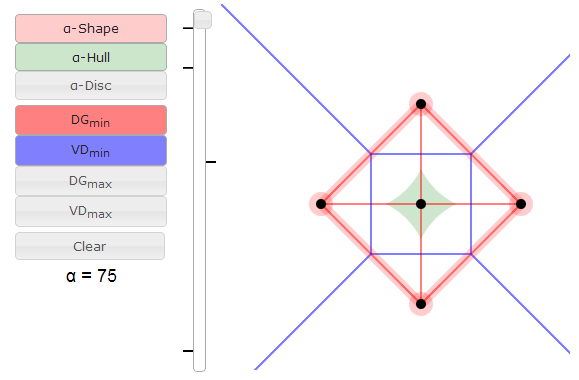
\includegraphics[scale=0.5]{../bilder/alphaShape_ui.png}
	\caption{Benutzeroberfläche der $\alpha$-Shapes HTML5-Applikation}
	\label{fig:alphaShape_ui}
\end{figure}

In Abbildung~\ref{fig:alphaShape_ui} ist die Benutzeroberfläche mit einigen aktivierten Anzeigemodi dargestellt.

Die Zeichenfläche besitzt zwei Eingabemodi. Der Punktmengenmodus ist aktiv, sofern der Anzeigemodus $\alpha$-Disc inaktiv ist. Im Punktmengenmodus können Punkte durch Links-Klick bzw. kurze Berührung eines Touchdisplays erstellt werden. Befindet sich im näheren Umkreises des Ereignisses schon ein Punkt, so wird dieser gelöscht. Durch Mouse- bzw. Touch-Drag-Ereignisse können Punkte verschoben werden. Mit dem Clear-Button können alle Punkte der Punktmenge gelöscht werden.

Im $\alpha$-Disc-Anzeige- und -Eingabemodus wird durch einen Links-Klick bzw. eine kurze Berührung der Mittelpunkt der $\alpha$-Disc verändert. Der Mittelpunkt kann auch durch Drag-Ereignisse verändert werden.

Der Parameter $\alpha$ kann über ein Slider-Steuerelement verändert werden. Auf einer Seite des Sliders befindet eine Markierung, welche dem Wert 0 entspricht. Auf der anderen Seite sind Markierungen angebracht, welche den Shape-Schwellen der Punktmenge entsprechen. Die Werte für $\alpha$ können mit einem Pixel Genauigkeit eingestellt werden.

\section{Mögliche Anwendungen}

Alle Anwendungen aus dem Kapitel über Shape-Spektrum-Algorithmen lassen sich mit der Applikation nachvollziehen. Für alle Beispiel-Probleme ist zu Beachten, dass sie nur im Rahmen der gegebenen Genauigkeit von einem Pixel gelöst werden können.

\begin{itemize}
\item Finden des dichtesten Paares: Ist der $\alpha$-Regler auf die kleinste, positive Markierung eingestellt, so sind die dichtesten Paare durch Kanten in der $\alpha$-Shape verbunden. Ein Beispiel dafür ist in Abbildung~\ref{fig:shapeHull_closestPair} dargestellt.

\item Finden des kleinsten einschließenden Kreises: Ist der $\alpha$-Regler auf die betragsmäßig kleinste, negative Markierung eingestellt, so ist der kleinste einschließende Kreis gleich dem Rand der $\alpha$-Hülle. Abbildung~\ref{fig:shapeHull_smallestCircle} stellt hierfür ein Beispiel dar.

\item Finden der konvexen Hülle: Ist der $\alpha$-Regler auf den größtmöglichen positiven oder negativen Wert eingestellt, so ist die $\alpha$-Hülle gleich der konvexen Hülle und die $\alpha$-Shape ist gleich dem Rand der konvexen Hülle. Auch hierzu gibt es ein Beispiel in Abbildung~\ref{fig:shapeHull_convex}.
\end{itemize}

Eine weitere mögliche Anwendung ist das Erkennen von Strukturen in verrauschten Bildern. Hierzu kann kein $\alpha$ angegeben werden, da diese Anwendung sehr von der Wahrnehmung des Benutzers abhängig ist.

\begin{figure}[htbp]
	\centering
	\subfloat[Verrauschtes Bild\label{fig:bigASNoise}]
		{
\includegraphics[scale=0.2]{../bilder/bigASNoise.png}}
	\hspace{2cm}
	\subfloat[Verrauschtes Bild mit $\alpha$-Shape\label{fig:bigASNoise_shape}]
		{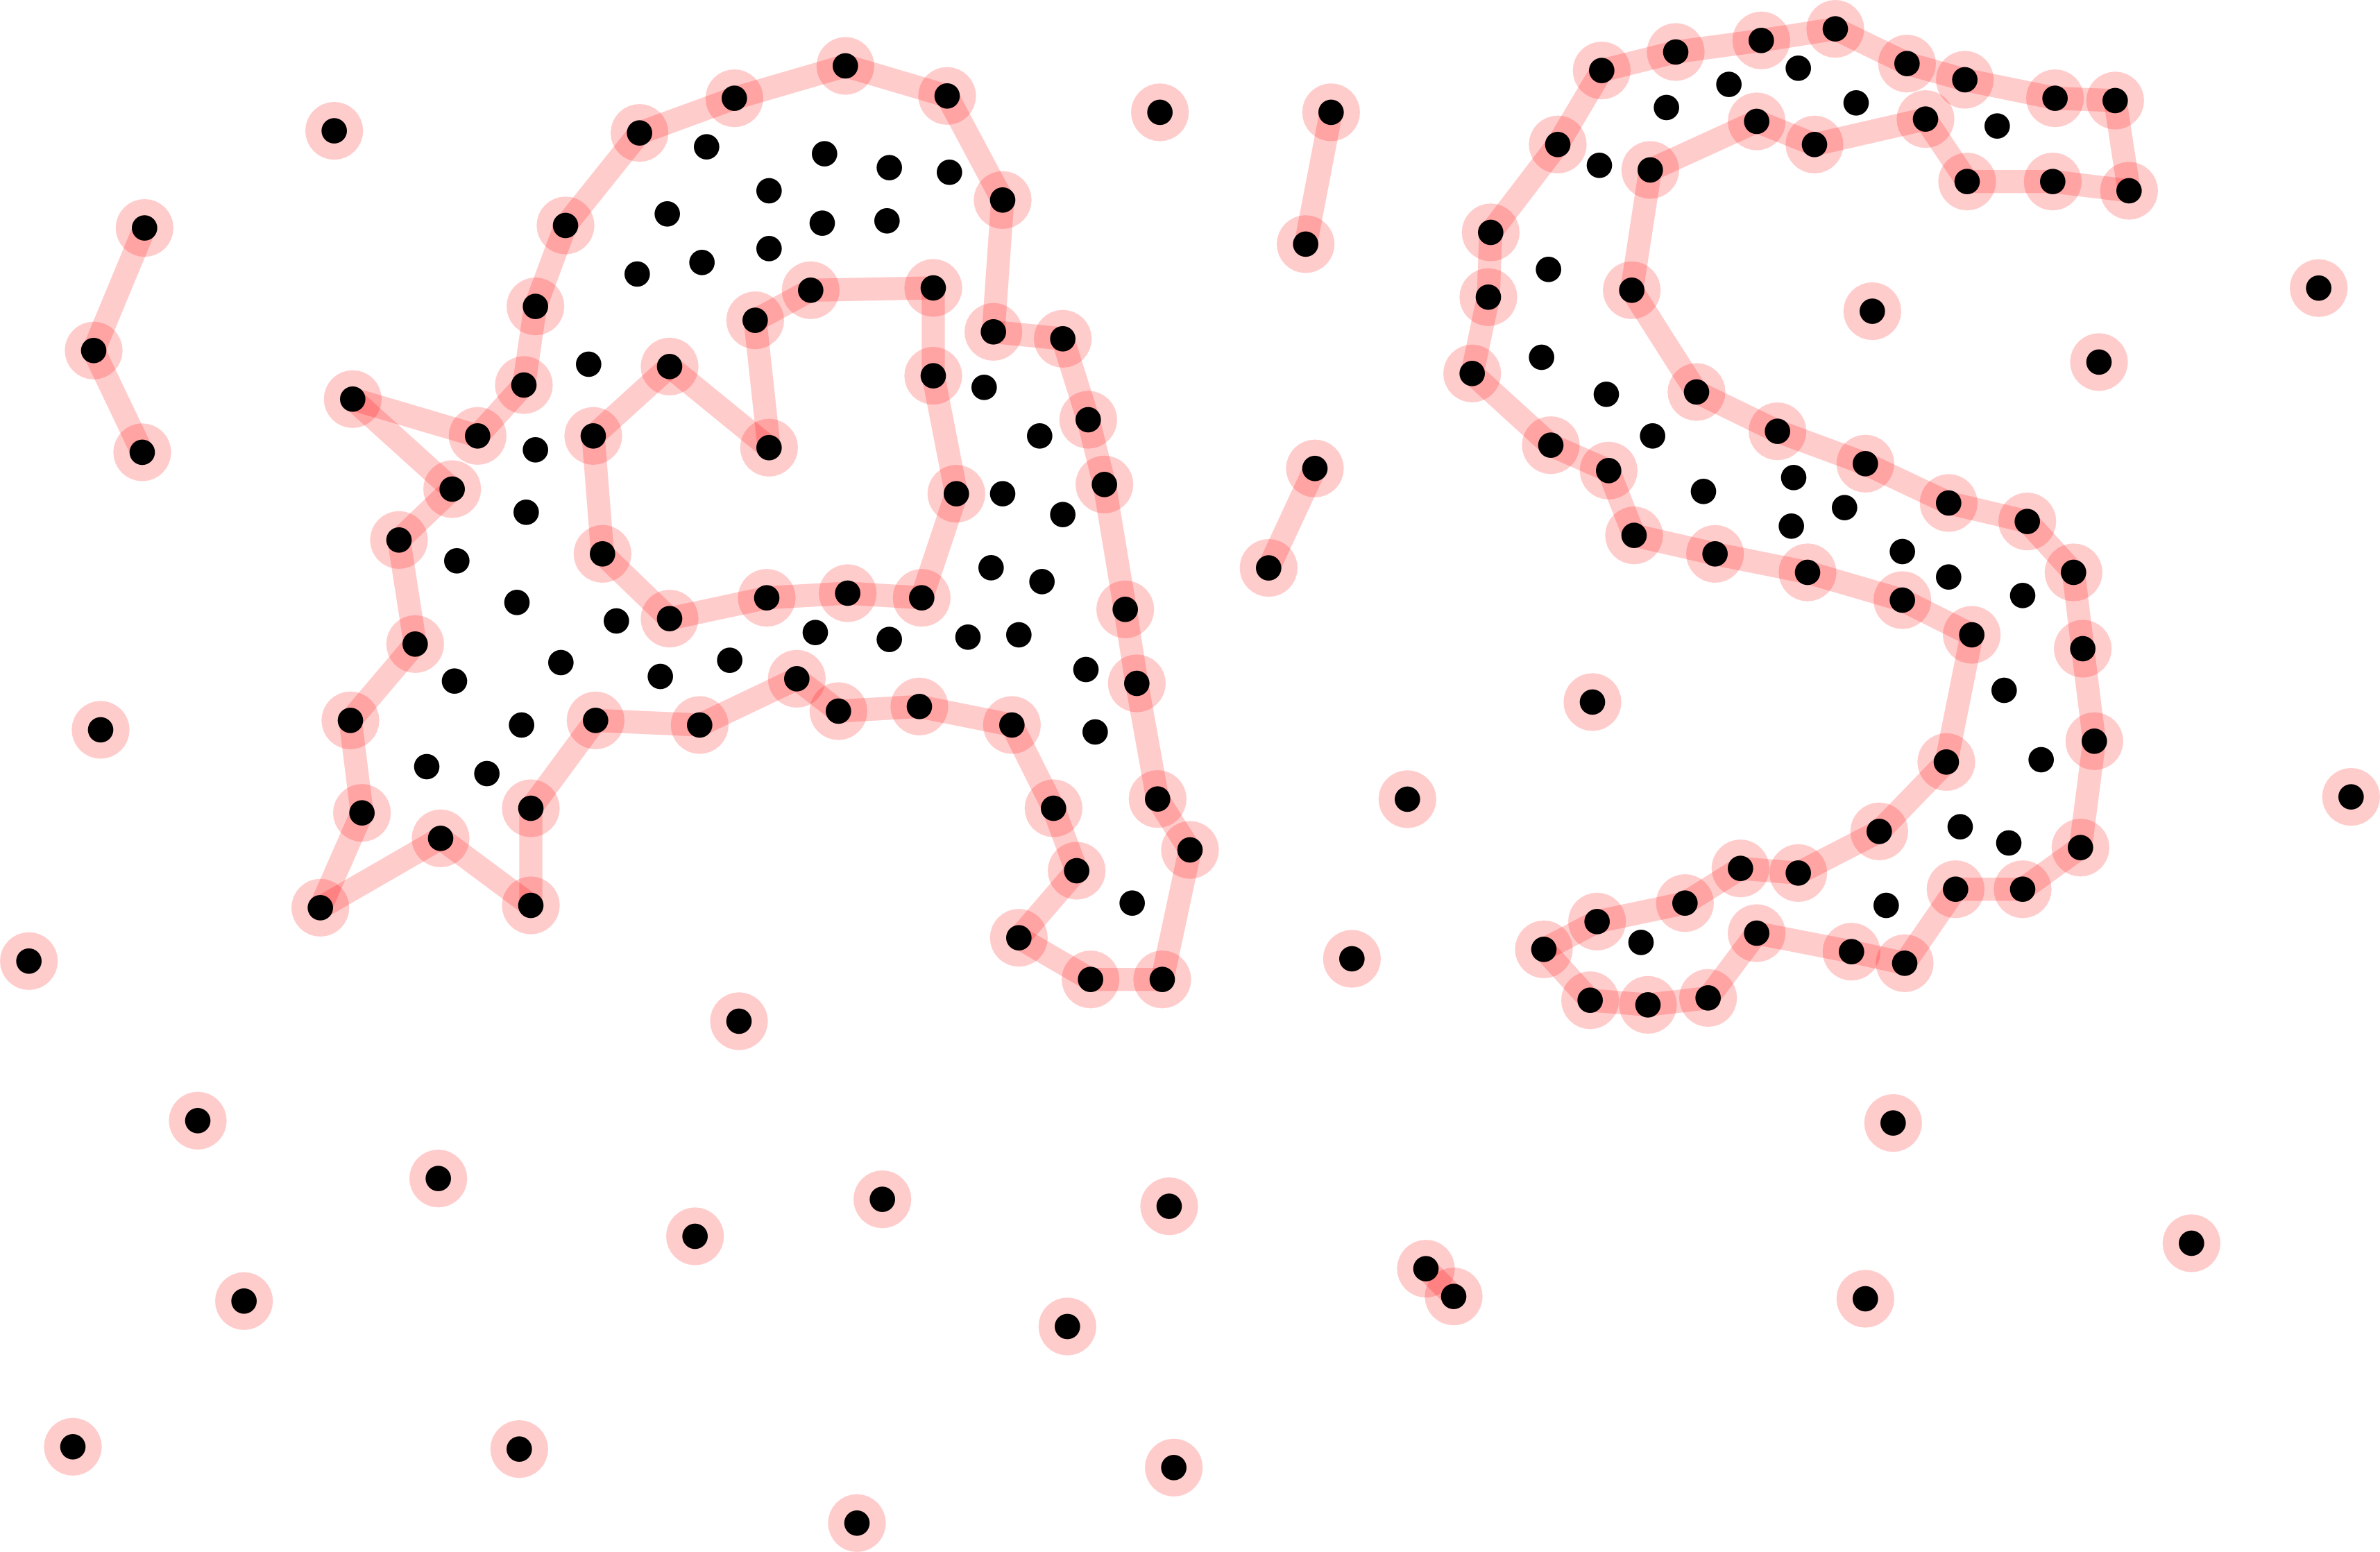
\includegraphics[scale=0.2]{../bilder/bigASNoise_shape.png}}
	\caption{Erkennung von Strukturen in verrauschten Bildern}
	\label{fig:pictureNoise}	
\end{figure}

Abbildung~\ref{fig:bigASNoise} zeigt das Beispiel der Gestalt der Buchstaben A und S. Hier wurden weitere Punkte eingefügt, welche als Rauschen interpretiert werden können. Abbildung~\ref{fig:bigASNoise_shape} zeigt die $\alpha$-Shape des verrauschten Bildes. Durch geschickte Wahl des Parameters $\alpha$ können $\alpha$-extreme Punkte mit Knotengrad 0 als Rauschen identifiziert werden. Die Erkennbarkeit der Buchstaben wird so deutlich erhöht.

Auch viele der in Kapitel \ref{alpha_props} gemachten Aussagen zu Eigenschaften von $\alpha$-Shapes können mit der Anwendung visualisiert werden. Hier seien nur ein paar Beispiele genannt.

\begin{itemize}
\item Die $\alpha$-Shape ist ein Subgraph des Delaunay-Graphen: Wählt man die Anzeigemodi $\alpha$-Shape, $DG_{\min}$ und $DG_{\max}$ aus und variiert $\alpha$ über den gesamten Wertebereich des Sliders, so kann man kann erkennen, dass jede Kante der Delaunay-Graphen für bestimmte $\alpha$ von einer Kante der $\alpha$-Shape überdeckt wird. Man kann auch erkennen, dass jede Kante der $\alpha$-Shape eine Kante eines Delaunay-Graphen überdeckt.

\item Man kann den eben beschriebenen Versuch auch getrennt für $DG_{\min}$ und positive $\alpha$ sowie für $DG_{\max}$ und negative $\alpha$ durchführen.

\item Bestimmung von $\alpha_{\max}$ für einen Knoten $P$ aus $DG_{\min}(S)$, welcher nicht auf dem Rand der konvexen Hülle liegt: Zu Beginn stellt man den Anzeigemodus $\alpha$-Shape ein und wählt $\alpha = 0$. Dann erhöht man $\alpha$ solange, bis $P$ nicht mehr rot umrandet ist. Der letzte angezeigte Wert von $\alpha$, für welchen $P$ noch rot umrandet war, ist $\lfloor \alpha_{\max} \rfloor$.

\item Bestimmen eines Knotens des Voronoi-Diagramms auf der Begrenzung von $VC_{\min}(P)$, welcher Abstand $\alpha_{\max}$ zu $P$ hat. $P$ darf dazu nicht auf dem Rand der konvexen Hülle liegen.  Hierzu werden zusätzlich zum letzten Versuch die Anzeigemodi $VD_{\min}$ und $\alpha$-Disc benötigt. Es muss $\alpha = \lfloor \alpha_{\max} \rfloor$ eingestellt werden. Dann wird der Mittelpunkt der $\alpha$-Disc nacheinander auf alle Knoten von $VD_{\min}(S)$, welche auf dem Rand von $VC_{\min}(P)$ liegen, platziert. Liegt $P$ für einen dieser Knoten auf dem Rand der Kreisscheibe, so ist ein Knoten mit Abstand $\alpha_{\max}$ zu $P$ gefunden.
\end{itemize} 

\section{Plattformspezifische Besonderheiten}

Da die Anwendung sowohl in einem Browser auf einem PC als auch auf mobilen Geräten, wie Smartphones oder Tablets, bedienbar sein soll, sind einige Dinge zu beachten.

Die Bedienelemente müssen groß genug sein um sie mit dem Finger bedienen zu können. Hierzu gibt es JavaScript-Bibliotheken, welche anpassbare Steuerelemente anbieten. Für die hier beschriebene Anwendung wurde die Bibliothek "`jQuery user interface"' benutzt, welche unter \autocite{jqueryui} zu finden ist. Alle Button-Steuerelement sowie der Slider stammen aus ihr. Für die Steuerelemente aus "`jQuery user interface"' sind die Event-Handler, welche eine Touchbedienung ermöglichen, nicht implementiert. Hierzu ist die Bibliothek "`jQuery UI Touch Punch"' notwendig, welche unter \autocite{jqueryuitouch} zu finden ist. Bei der Zeichenfläche ist darauf zu achten, selbst die Event-Handler für Mouse- und Touch-Events zu implementieren.

Weiterhin ist zu Beachten, dass mobile Geräte in der Anzeigegröße sehr eingeschränkt sind. Auch kann ein solches Gerät in zwei verschiedenen Ausrichtungen, Hoch- und Querformat, bedient werden. Auch ein Browser-Fenster auf einem PC kann verschiedene Größen sowie Hoch- und Querformat annehmen.

Wird diese Anwendung in einem Fenster im Querformat ausgeführt, so werden die Button- und Slider-Bedienelemente links und die Zeichenfläche rechts dargestellt. Die Buttons werden untereinander und der Slider wird rechts daneben, vertikal dargestellt. Hat das Fenster eine ausreichende Höhe, so werden alle Bedienelemente dargestellt. Ist die Höhe des Fensters kleiner als eine gewisse minimale Höhe, so werden die Bedienelemente für Delaunay-Graphen und Voronoi-Diagramme nicht dargestellt.

\begin{figure}[htbp]
	\centering
	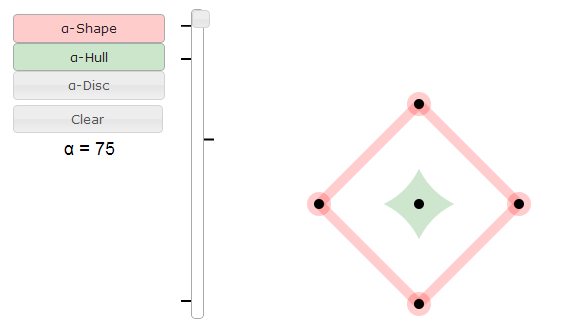
\includegraphics[scale=0.5]{../bilder/alphaShape_uiMin.png}
	\caption{Minimale Benutzeroberfläche der $\alpha$-Shapes HTML5-Applikation}
	\label{fig:alphaShape_uiMin}
\end{figure}

Abbildung~\ref{fig:alphaShape_uiMin} zeigt die Anwendung im Querformat mit ausgeblendeten Eingabemöglichkeiten.

Wird die Anwendung in einem Fenster im Hochformat ausgeführt, so werden nur die Buttons für $\alpha$-Shape, -Hülle, und -Kreisscheibe sowie der Slider dargestellt. Diese Bedienelemente werden oben dargestellt und die Zeichenfläche unten. Je nach Breite des Fensters werden die Buttons nebeneinander oder untereinander dargestellt. Der Slider wird unter den Buttons horizontal dargestellt.

\begin{figure}[htbp]
	\centering
	\subfloat[Darstellung im Hochformat\label{fig:alphaShape_uiVertNoBreak}]
		{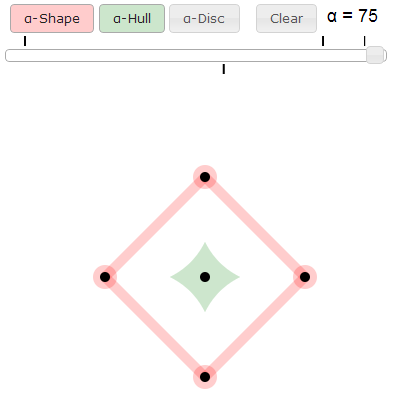
\includegraphics[scale=0.4]{../bilder/alphaShape_uiVertNoBreak.png}}
	\hspace{2cm}
	\subfloat[Darstellung im Hochformat mit Umbruch\label{fig:alphaShape_uiVertBreak}]
		{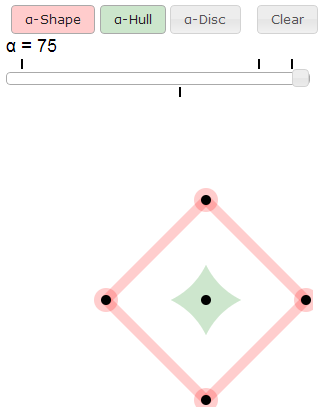
\includegraphics[scale=0.4]{../bilder/alphaShape_uiVertBreak.png}}
	\caption{Darstellung der Benutzeroberfläche im Hochformat}
	\label{fig:alphaShape_uiVert}	
\end{figure}

In Abbildung~\ref{fig:alphaShape_uiVert} wird die Benutzeroberfläche im Hochformat mit und ohne Umbruch der Anzeigeelemente dargestellt.

Wie diese plattformspezifischen Besonderheiten im einzelnen mit HTML5 realisiert werden ist im Anhang beschrieben. Dort wird auch auf Besonderheiten bei der Entwicklung mit JavaScript im Vergleich zu Java eingegangen.

% !TEX encoding = UTF-8 Unicode

\chapter{Zusammenfassung und Ausblick}

$\alpha$-Shapes sind Graphen, welche benutzt werden können um Gestalten in Punktmengen zu identifizieren. Die Güte der Darstellung einer Gestalt hängt von dem Parameter $\alpha$ ab. Die $\alpha$-Shape ist eng verwandt mit der $\alpha$-Hülle, welche eine flächenmäßige Darstellung von Gestalten in Punktmengen ist und eine Verallgemeinerung der konvexen Hülle darstellt.

Die $\alpha$-Shape ist ein Subgraph des Delaunay-Graphen. Die Entscheidung, welche Knoten und Kanten des Delaunay-Graphen auch Knoten und Kanten der $\alpha$-Shape sind, wird mit Hilfe des Voronoi-Diagramms getroffen. Diese Eigenschaft wurde ausgenutzt um einen Algorithmus zur Bestimmung der $\alpha$-Shape zu beschreiben. Auch andere Eigenschaften von Punktmengen lassen sich mit diesem Algorithmus bestimmen.

Die Algorithmen zur Bestimmung von Voronoi-Diagrammen und $\alpha$-Shape wurden in JavaScript implementiert und damit eine HTML5-Anwendung zur Veranschaulichung der $\alpha$-Shape entwickelt. Zusätzlich können $\alpha$-Hülle, Voronoi-Dia\-gramm und Delaunay-Graph eingeblendet werden. Mit der Darstellung von $\alpha$-Shapes in dieser Applikation können besondere Eigenschaften von Punktmengen sowie markante Punkte bestimmt werden. Bei der Entwicklung der Applikation wurde Wert darauf gelegt, dass sie sowohl auf dem PC als auch auf mobilen Geräten ausführbar und bedienbar ist.

Die $\alpha$-Shape kann, genauso wie Voronoi-Diagramm und Delaunay-Graph, nicht nur in der Ebene sondern auch im Raum definiert werden. Hierbei übernehmen $\alpha$-Kugeln die Rolle der $\alpha$-Kreisscheiben. Mit der 3D-$\alpha$-Shape können Strukturen in 3D-Punktmengen erkannt werden.

Auch hierzu wäre eine HTML5-Anwendung denkbar. Die graphische Repräsentation könnte durch den WebGL-Standard realisiert werden.


\appendix
% !TEX encoding = UTF-8 Unicode

\chapter{HTML5-Anwendungsentwicklung}

Wird eine Anwendung mit HTML5 entwickelt, so wird eine Kombination der drei Technologien HTML, CSS und JavaScript verwendet. Jede dieser Technologien deckt einen gewissen Aspekt der HTML5-Anwendungsentwicklung ab. HTML wird verwendet um Inhalte festzulegen, mit CSS wird das Layout festgelegt und JavaScript bestimmt das Verhalten. Soweit möglich sollte diese Trennung auch eingehalten werden. Da Inhalt und Layout aber auch dynamisch angepasst werden, greift JavaScript auch in diese Bereiche ein.

\section*{Dynamische Anpassung der Benutzeroberfläche}

Wenn im Bezug auf die vorliegende HTML5-Anwendung von Inhalt gesprochen wird, so sind damit die Steuerelemente selbst sowie ihre Gruppierung gemeint. Das Layout bestimmt die Anordnung der Steuerelemente und welche Steuerelemente angezeigt werden. Im vorherigen Abschnitt ist angesprochen worden, dass sich die Anzahl der angezeigten Steuerelemente sowie ihr Layout je nach Fenstergröße ändert. Diese Änderung wird mittels JavaScript durchgeführt. Die Bibliothek jQuery \autocite{jquery} bietet eine Funktion, mit welcher sich einzelne oder mehrere HTML-Elemente über CSS-Selektoren auswählen lassen. Die HTML-Attribute und CSS-Eigenschaften der selektierten Elemente können dann manipuliert werden. Die jQuery-Funktion wird entweder mit \verb+jQuery+ oder dem Dollar-Zeichen aufgerufen.

\begin{figure}[htbp]
	\centering
	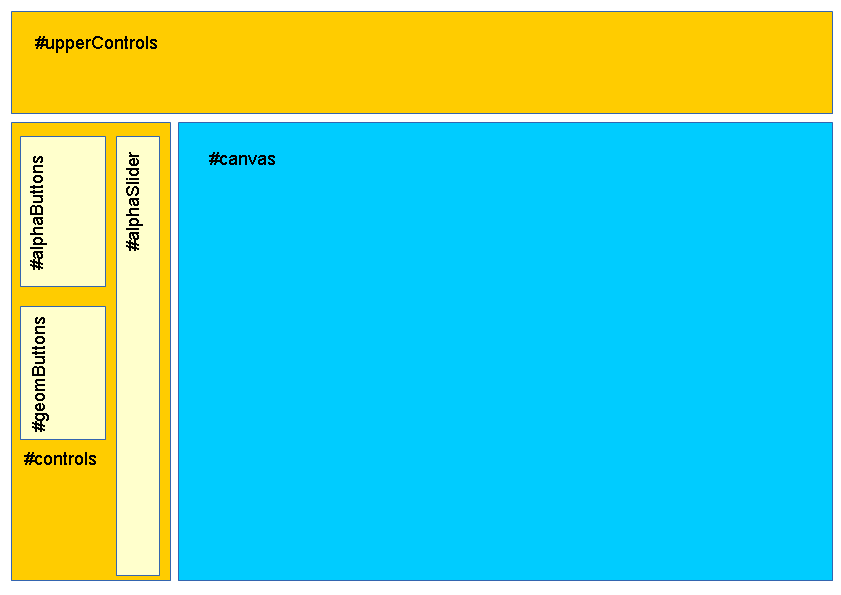
\includegraphics[scale=0.9]{../bilder/layout.png}
	\caption{Layout der $\alpha$-Shapes HTML5-Applikation}
	\label{fig:layout}
\end{figure}

In Abbildung~\ref{fig:layout} ist das Layout der Applikation dargestellt. Die Bezeichner mit einer vorangestellten Raute beziehen sich auf IDs von HTML-Elementen. Die Raute wird CSS-Selektoren vorangestellt, welche ein Element nach ihrer ID auswählen. Die in Gelbtönen eingefärbten Blöcke stellen Div-Elemente dar. Der blaue Block ist das Canvas-Element, auf welchem die Punktmenge und alle anderen Diagramme gezeichnet werden. In \verb+alphaButtons+ sind alle Buttons enthalten, welche die Darstellung von $\alpha$-Shape, -Hülle und -Kreisscheiben steuern. In \verb+geomButtons+ sind alle Buttons enthalten, welche die Darstellung von Delaunay-Graphen und Voronoi-Diagrammen steuern.

Das nun gezeigte Codebeispiel befindet sich in dem Resize-Event-Handler des Window-Elements. In Listing~\ref{upperSideControls} wird demonstriert, wie zwischen Darstellung im Hoch- und Querformat bzw. zwischen seitlichen und oberen Steuerelementen umgeschaltet wird. Hierzu sei angemerkt, dass alle Buttons in \verb+geomButtons+ zu einer Klasse \verb+geomButton+ gehören. CSS-Selektoren, welche sich auf eine Klasse beziehen, wird ein Punkt vorangestellt.

\begin{lstlisting}[float = htbp, caption={Umstellen zwischen Hoch- und Querformat},label=upperSideControls]
if (window.innerHeight > window.innerWidth) {
	$('.geomButton').prop('checked', false);
	$('.geomButton').button('refresh');
	$('#upperControls').css('display', '');
	$('#controls').css('display', 'none');
} else {
	$('#upperControls').css('display', 'none');
	$('#controls').css('display', '');        
}
\end{lstlisting}

Die jQuery-Funktion liefert ein jQuery-Objekt zurück. Mit den Methoden \verb+prop+ und \verb+css+ können HTML-Attribute bzw. CSS-Eigenschaften von den durch das jQuery-Objekt selektierten Elementen verändert werden. Die Methode \verb+button+ wird durch die Bibliothek jQueryUI hinzugefügt. Die verwendeten Button-Steuer\-elemente sind eigentlich HTML-Checkbox-Elemente. Mit jQueryUI können diese als Toggle-Buttons dargestellt werden, welche durch ihre Größe besser mit dem Finger zu bedienen sind. Da in der Darstellung im Hochformat die Buttons für Delaunay-Graphen sowie Voronoi-Diagramme nicht sichtbar sind, wird die Darstellung dieser Diagramme deaktiviert.

\section*{Event-Handler für Touch- und Mausbedienung}

Da mobile Geräte über Touchdisplays bedient werden, müssen die entsprechenden Event-Handler implementiert werden.

\begin{lstlisting}[float = htbp, caption={Zuweisen der Event-Handler an das Canvas-Element},label=canvasEvents]
$('#canvas').mousedown(CanvasController.handleDragStart);
$('#canvas').mousemove(CanvasController.handleDragMove);
$('#canvas').mouseup(CanvasController.handleDragEnd);

$('#canvas').bind('touchstart',
	CanvasController.handleTouchDragStart);
$('#canvas').bind('touchmove',
	CanvasController.handleTouchDragMove);
$('#canvas').bind('touchend',
	CanvasController.handleTouchDragEnd);
\end{lstlisting}

Listing~\ref{canvasEvents} zeigt die Zuweisung der Event-Handler für Mouse- und Touch-Ereignisse. Die Implementierung dieser Event-Handler-Funktionen ist aber fast identisch. Sie unterscheiden sich nur in der Ermittlung der Position des Ereignisses und ob an dieser Position schon ein Punkt existiert. Für Touchbedienung müssen ggf. mehrere Touch-Ereignisse (für mehrere Finger) ausgewertet werden und Punkte in einem größeren Umkreis um die Position des Events berücksichtigt werden.

\begin{lstlisting}[float = htbp, caption={Touch-Event-Handler},label=touchEvent]
var x = event.originalEvent.targetTouches[0].pageX -
	$('#canvas').offset().left;
var y = event.originalEvent.targetTouches[0].pageY -
	$('#canvas').offset().top;
var pointIndex = Misc.getIndexOfElementWithMinimalDistance(
	UserData.points, new Vector(x, y), Vector.calcDist,
	CanvasController.maxPointDistTouch);
\end{lstlisting}

Listing~\ref{touchEvent} zeigt die Ermittlung der Koordinaten eines Touch-Events sowie die Ermittlung des Index des Punkts in einem Array, welcher am nächsten zu den Koordinaten des Ereignisses liegt. Falls der Abstand des nächsten Punktes einen Maximalwert überschreitet oder das Array leer ist, wird der Wert $-1$ zurückgegeben. \verb+UserData.points+ ist das Array mit den Vektoren der Punkte, welche auf der Zeichenfläche dargestellt werden. Mit \verb+new Vector(x, y)+ wird ein Vektor mit den Koordinaten des Events zum Vergleich mit den Array-Elementen erzeugt. \verb+Vector.calcDist+ ist eine Funktion, welche die Distanz zwischen Vektoren berechnet. Die Konstante \verb+CanvasController.maxPointDistTouch+ legt den Radius des Umkreises fest, in welchem ein Punkt mittels einer Berührung selektiert werden kann. 

\section*{JavaScript und Klassen}
In der Entwicklung objektorientierter Software wird Code üblicherweise in Klassen organisiert. JavaScript bietet dieses Konstrukt nicht an. Allerdings lassen sich durch JavaScript-Spracheigenschaften Klassen nachbilden. Dies wird z.B. in \autocite{Flanagan2011} beschrieben. Listing~\ref{vectorClass} zeigt eine Klasse \verb+Vector+ mit den Attributen \verb+x+ und \verb+y+, einer Methode \verb+add+ und einer statischen Methode \verb+calcDist+.

\begin{lstlisting}[float = htbp, caption={Eine Vektor-Klasse},label=vectorClass]
function Vector(x, y) {
    this.x = x;
    this.y = y;    
};

Vector.prototype = {
    constructor: Vector,
    add : function(v) {
        return new Vector(this.x + v.x, this.y + v.y);
    }, ...
};

Vector.calcDist = function(v1, v2) {
    var dist = v1.sub(v2).abs();
    return dist;
};
\end{lstlisting}

Die Funktion \verb+Vector+ wird Konstruktor genannt. In ihr werden die Attribute festgelegt. Im Prototypen werden die Methoden definiert. Statische Methoden werden dem Konstruktor als Eigenschaft hinzugefügt.

Zudem lassen sich in Klassen auch zusätzliche Einschränkungen wie Sichtbarkeit und Veränderbarkeit von Objekt- und Klasseneigenschaften definieren. JavaScript bietet diese Möglichkeiten nicht. Sichtbarkeit und Veränderbarkeit können durch jsDoc-Kommentare, wie in \autocite{useJsDoc} beschrieben, festgelegt werden. jsDoc wird ähnlich wie JavaDoc verwendet. Ein Compiler, wie z.B. der hier verwendete Closure-Compiler von Google \autocite{closureTools}, kann die Einhaltung von Sichtbarkeit und Veränderbarkeit überprüfen, sie kann aber nicht durch den Interpreter erzwungen werden. Listing~\ref{vectorClassImmutable} zeigt wie die Attribute der Klasse \verb+Vector+ zu Konstanten gemacht werden können.

\begin{lstlisting}[float = htbp, caption={Eine Vektor-Klasse mit konstanten Attributen},label=vectorClassImmutable]
function Vector(x, y) {
    /**
     * @const
     */
    this.x = x;
    /**
     * @const
     */
    this.y = y;    
};
\end{lstlisting}

\section*{JavaScript und Typsicherheit}

JavaScript ist eine dynamisch typisierte Sprache, welche Duck-Typing benutzt. Das bedeutet, es können zur Laufzeit Eigenschaften zu Objekten hinzugefügt werden und der Interpreter prüft erst zur Laufzeit, ob ein Objekt eine benötigte Eigenschaft besitzt. Ist eine benötigte Eigenschaft nicht vorhanden, so kommt es zu einem Laufzeitfehler.

Mit Hilfe der vorher schon benutzten jsDoc-Kommentare können Typinformationen zu Variablen hinzugefügt werden. Ein Compiler kann dann überprüfen, ob den so deklarierten Variablen auch Objekte des richtigen Typs zugewiesen werden und ob das Objekt über die benötigten Eigenschaften verfügt. Listing~\ref{vectorClassTypes} zeigt wie der Klasse \verb+Vector+ Typinformationen hinzugefügt werden können.

\begin{lstlisting}[float = htbp, caption={Eine Vektor-Klasse mit Typinformationen},label=vectorClassTypes]
/**
 * Represents a 2D vector.
 * 
 * @constructor
 * @param {number} x coordinate
 * @param {number} y coordinate
 */
function Vector(x, y) {
    /**
     * @const
     * @type number
     */
    this.x = x;
    /**
     * @const
     * @type number
     */
    this.y = y;    
};
...
    /**
     * Vector addition
     * 
     * @param {Vector} v 2nd summand
     * @returns {Vector} sum of this vector and v
     */
    add : function(v) {
        return new Vector(this.x + v.x, this.y + v.y);
    },
...
\end{lstlisting}

Zusätzlich zu den Typinformationen wurden der Konstruktor- und die Methoden-Köpfe auch noch kommentiert. Das jsDoc-Projekt stellt ein Tool \autocite{jsDoc} zur Verfügung, mit welchem aus dem kommentierten Quellcode eine API-Dokumentation im HTML-Format erstellt werden kann.

\section*{JavaScript Unit-Tests} 

Eine andere Möglichkeit vor der Ausführung des Programms Fehler zu erkennen sind Unit-Tests. Die Bibliothek Jasmine \autocite{jasmine} ermöglicht das Erstellen und Ausführen von Unit-Tests. Listing~\ref{vectorClassUnitTest} zeigt einen Unit-Test zur \verb+add+-Methode der \verb+Vector+-Klasse.

\begin{lstlisting}[float = htbp, caption={Ein Unit-Test zur Vektoraddition},label=vectorClassUnitTest]
describe('Vector', function() {
    it('adds vectors', function() {
        var vector1 = new Vector(5,7);
        var vector2 = new Vector(1,2);
        var expected = new Vector(6,9);
        var result = vector1.add(vector2);
        
        expect(expected.equals(result)).toBe(true);
    });
});
\end{lstlisting}


\section*{JavaScript Vererbung}

In der Entwicklung objektorientierter Software wird üblicherweise zwischen der Implementierungs- und der Schnittstellenvererbung unterschieden. JavaScript unterstützt das Konzept der Prototypen-basierten Vererbung. Damit können Implementierungen vererbt werden. Dies wird auch in \autocite{Flanagan2011} beschrieben. 


\begin{lstlisting}[float = htbp, caption={Eine AVL-Baum-Klasse},label=treeClass]
/**
 * @constructor
 */
function Tree() {
...
};
Tree.prototype = {
	constructor: tree;
	...
};

/**
 * @constructor
 * @extends Tree
 */
function FortuneTree() {
...
};

FortuneTree.prototype = Object.create(Tree.prototype);
FortuneTree.prototype.constructor = FortuneTree;

FortuneTree.prototype.insertNewArcNode =
	function(eventLocation, edgeList) {
...
}
\end{lstlisting}

Listing~\ref{treeClass} zeigt eine Klasse \verb+Tree+, von welcher eine Klasse \verb+FortuneTree+ abgeleitet ist. Bei \verb+Tree+ handelt es sich um einen AVL-Baum. In Fortunes Algorithmus werden innere Knoten und Blätter unterschieden. Das Einfügen eines Knotens in den AVL-Baum in Fortunes Algorithmus umfasst einige sehr spezielle Schritte. Darum ist das einfügen eines Knotens in der speziellen \verb+FortuneTree+-Klasse implementiert.

\chapter{Projektstruktur}

Alle der im vorhergehenden Kapitel beschriebenen Hilfsmittel bei der Entwicklung mit HTML5 bzw. JavaScript finden sich in der Projektstruktur wieder. Das HTML5-Anwendungsprojekt ist im Repository \verb+AlphaShapeSeidinger+ unter \verb+projekte/alpha_shapes_html5+ zu finden. Der wichtigste Ordner unterhalb dieses Ordners ist der Ordner \verb+public_html+. In ihm befinden sich alle HTML-, CSS- und JavaScript-Dateien. Hier wird kurz der Inhalt von \verb+public_html+ beschrieben:

\begin{itemize}
\item \verb+index.html+: Einbindung der CSS-Stylesheets und aller JavaScript-Dateien, Definition aller Steuerelement sowie deren Gruppierung
\item \verb+css/custom-ui.css+: Definition aller statischen Layout-Aspekte
\item \verb+data/simple_point_set.json+: Initiale Punkt\-menge im JSON-For\-mat
\item \verb+js/libs+: Alle eingesetzten JavaScript-Bibliotheken
\item \verb+js/geom+: Geometrische Datentypen
\item \verb+js/ds+: Datenstrukturen
\item \verb+js/algo+: Algorithmen
\item \verb+js/util+: Hilfsfunktionen
\item \verb+js/ui+: Event-Handler
\item \verb+js/compiled+: Compiler-generierter JavaScript-Code
\item \verb+js/README.md+: Quelle für Index-Seite der jsDoc-API-Dokumentation
\item \verb+test+: Jasmine Bibliothek sowie Unit-Tests
\item \verb+test/SpecRunner+: HTML-Datei zum Ausführen der Unit-Tests
\end{itemize}

Die vorher beschriebenen Werkzeuge befinden sich im Ordner des Anwendungsprojekts unterhalb des Ordners \verb+tools+:

\begin{itemize}
\item \verb+closure/compiler.jar+: Closure-Compiler
\item \verb+jsdoc/jsdoc+: Tool zur Erstellung von jsDoc-API-Dokumentation
\item \verb+check.bat+: Führt den Closure-Compiler mit einem hohen Warning-Level aus.
\item \verb+compile.bat+: Führt den Closure-Compiler mit den Standard-Einstellungen aus und legt das Ergebnis in das JavaScript-Quellcode-Verzeichnis.
\item \verb+doc.bat+: Führt das jsDoc-Tool aus und legt die API-Dokumentation in das Verzeichnis \verb+public_html/api+. Dieses Verzeichnis wird von Subversion ignoriert.
\end{itemize}


\printbibliography
\listoffigures

\end{document}
